\documentclass[a4paper, 12pt, oneside]{report}
\usepackage[T1]{fontenc}
\usepackage[utf8]{inputenc}
\usepackage{lmodern}
\usepackage{layout}
\usepackage{emptypage}
\usepackage{fancyhdr}
\usepackage[spanish,activeacute]{babel}
%\usepackage[Conny]{fncychap}
%\usepackage{graphicx}
\usepackage{subfigure} % subfiguras
\usepackage{caption}
\usepackage{mathtools}
\usepackage{hyperref}
\usepackage[a4paper,top=3cm, bottom=3cm, inner=2.5cm, outer=2.5cm]{geometry}
\usepackage{listings}
\usepackage[spanish]{babel}
\usepackage{url}
\usepackage{float}
\usepackage{multirow}
\usepackage{rotating} 
\usepackage{color}
\usepackage{colortbl}
\usepackage[table]{xcolor}
\usepackage[spanish]{babel}
\usepackage{enumerate}
\usepackage{enumitem}
\usepackage{multicol}
\usepackage{mwe}
\usepackage[acronym, nonumberlist]{glossaries}
\makeglossaries

\makeatletter
\renewcommand{\@makeschapterhead}[1]{%
%  \vspace*{50\p@}%
  \vspace*{0\p@}%
  {\parindent \z@ \raggedright
    \normalfont
    \interlinepenalty\@M
    \Huge \bfseries  #1\par \nobreak
%    \vskip 40\p@
    \vskip 15\p@
  }}
\makeatother

\renewcommand{\baselinestretch}{1.4}
\setlength{\headheight}{16pt} 
\captionsetup{justification=justified}
\pretolerance=1000

\chead[]{}
\rhead[]{}
\renewcommand{\headrulewidth}{0.5pt}

\pagestyle{empty}

\title{Pr�cticas Docentes de Rob�tica en el Entorno JdeRobot-Academy}
\author{Carlos Awadallah Est�vez}

\lstset{
	float=hbp,
	basicstyle=\ttfamily\small,
	columns=flexible,
	tabsize=4,
	frame=single,
	extendedchars=true,
	showspaces=false,
	showstringspaces=false,
	numbers=none,
	numberstyle=\tiny,
	breaklines=false,
	breakautoindent=true,
	captionpos=b
}
\setcounter{tocdepth}{4}
\setcounter{secnumdepth}{4}

\definecolor{lightgray}{gray}{0.9}

\begin{document}
%%%%%%%%%%%%%%% Portada %%%%%%%%%%%%%%%%%%%%
\begin{titlepage}
	\begin{center}
		\vspace*{3mm}
		\begin{center}
			
\includegraphics[width=0.4\linewidth]{figures/logo.jpg}
		\end{center}
		\vspace{6.5mm}
		
		\fontsize{15.5}{14}\selectfont ESCUELA TÉCNICA SUPERIOR DE INGENIERÍA DE TELECOMUNICACIÓN
		\vspace{13mm}
		
		\fontsize{14}{14}\selectfont GRADO EN INGENIERÍA EN SISTEMAS \\ AUDIOVISUALES Y MULTIMEDIA
		
		\vspace{70pt}
		
		\fontfamily{lmss}\fontsize{15.7}{14}\selectfont \textbf{TRABAJO FIN DE GRADO} 
		
		\vspace{25mm}
		\begin{huge}
			Prácticas Docentes de Robótica en el Entorno \\ \vspace{0.4cm} JdeRobot-Academy
		\end{huge}
		
		\vspace{25mm}
		
		\begin{large}
			Autor: Carlos Awadallah Estévez
			
			Tutor: José María Cañas Plaza
			
			\vspace{10mm}
		\end{large}
		\begin{normalsize}
			Curso académico 2017/2018		
		\end{normalsize}
		\vspace{10mm}
		
	\end{center}
	
\end{titlepage}




\pagenumbering{Roman}

%%%%%%%%%%%%%%% Agradecimientos %%%%%%%%%%%%
\newgeometry{top=1.6cm,left=2cm,right=2cm}
\chapter*{Agradecimientos}
\setlength{\parskip}{1ex}

Tenía muchas ganas de escribir esta parte del trabajo, ya que me brinda una oportunidad increíble para agradecer a todos aquellos que han estado a mi lado por el apoyo, el sustento (anímico y también económico) y la orientación que me han regalado sin esperar nada a cambio.

La primera persona en quien pienso es en mi madre, mi pilar de apoyo para seguir adelante y, sobre todo, mi referente en la vida. A ella le dedico este trabajo, espero que estas simples frases sirvan para hacerle ver que le estoy muy agradecido, y que no tengo palabras para expresar lo que siento hacia ella. También al resto de mi familia, mi hermana Shadia, mi tía Rosi y mi abuela MªRosa por sus continuos mensajes de apoyo, sin ellos no habría llegado donde estoy. También a Antonio, que siempre estuvo ahí, que fue la persona que me dio la oportunidad de estudiar lo que quería con su generosidad. A todos ellos, y también a todos mis demás familiares, gracias por todo.

Sigo con mi tutor José María, sin el cual nada de esto habría sido posible. Depositó su confianza en mí, aguantó pacientemente mis continuas preguntas e inquietudes y me orientó siempre que lo necesité para sacar el proyecto adelante. Gracias por tu dedicación, y también por transmitirme el gusto por la robótica durante el trabajo, las prácticas y las clases del grado, campo en el que probablemente enfocaré mi futuro profesional.

Gracias a mi pareja, Bea, que estuvo ahí absolutamente todos los días, que aunque nos separasen 2500 km de distancia siempre estuvo tan cerca como Diciembre de Enero. Por todos los mensajes, por todas las charlas de Skype y por todas y cada una de las palabras intercambiadas que, aunque nunca te lo dije, fueron vitales para seguir aquí día a día con ilusión. Muchas gracias por estos 4 años de apoyo, que se dice pronto.

Como olvidarme de mis amigos de siempre, en especial de Joel C., Joel Y. y Ricardo, y de mi amiga Lidia. Siempre supieron sacar lo mejor de mí, y nada cambió cuando pasamos a vernos sólo unas pocas veces al año. Por todos los momentos compartidos, que me han hecho llegar a ser quien soy.

Por último, pero no por ello menos importantes, mencionar a todas las personas que conocí en Madrid. A todos ustedes: gracias. Esto no habría sido fácil si no hubieran hecho más amena la vida cotidiana. A mis chicos y chicas de la universidad y a mis chicas del gimnasio, un fuerte abrazo.
\restoregeometry


%%%%%%%%%%%%%%% Resumen %%%%%%%%%%%%%%%%%%%%
\chapter*{Resumen}
\setlength{\parskip}{1ex}

La robótica ha experimentado un crecimiento exponencial en los últimos tiempos, lo que se traduce en una acentuada presencia en la vida cotidiana y profesional, siendo cada vez más y más importante especialistas formados en esta materia. Así, surgen recientemente entornos que acercan a los alumnos de distintas etapas la posibilidad de adquirir competencias en robótica, como JdeRobot-Academy, que pone a disposición de los estudiantes universitarios varios ejercicios clásicos de la robótica de forma sencilla, completa y eficaz.

Este proyecto se ha centrado en la elaboración de dos nuevas prácticas para JdeRobot-Academy. Para cada una de ellas se ha preparado una infraestructura (con robot real o simulado), un nodo académico, la comunicación que resuelve con robot y la interfaz gráfica, permitiendo a potenciales alumnos abstraerse de las complejidades involucradas y así centrarse en el algoritmo oportuno. También se han desarrollado sendas soluciones de referencia. 

La primera de las prácticas es \textit{``Follow Face''}, que permitirá al alumno trabajar con hardware real (cámara Sony Evi d100p) y adquirir conocimientos de procesado de imagen, empleando clasificadores en cascada para discernir si una imagen de entrada al sistema contiene caras o no, y en caso afirmativo las persiga usando un control visual reactivo.

La segunda práctica, \textit{``Laser Loc''}, busca resolver un problema de localización basada en láser, en el cual el estudiante deberá valerse del método de filtro de partículas para lograr que un robot estime su posición con errores tolerables en un mundo conocido, del cual se proporciona un mapa binario.
\cleardoublepage

%%%%%%%%%%%%%%% �ndices %%%%%%%%%%%%%%%%%%%%
%\cleardoublepage
\renewcommand{\tablename}{Tabla}
%\renewcommand{\listtablename}{�ndice de tablas}
%\tableofcontents

%\cleardoublepage % ͭndice de figuras
%\addcontentsline{toc}{chapter}{\listfigurename}
%\listoffigures

%\cleardoublepage % ͭndice de tablas
%\addcontentsline{toc}{chapter}{�ndice de tablas}
%\listoftables 
\cleardoublepage
\tableofcontents % indice de contenidos

%\cleardoublepage
%\listoffigures % indice de figuras
%\addcontentsline{toc}{chapter}{\'Indice de figuras} % para que aparezca en el indice de contenidos

%%%%%%%%%%%%%%% Acronimos %%%%%%%%%%%%%%%%%%%%
%\addcontentsline{toc}{chapter}{Acr\'onimos}
\chapter*{Acrónimos}

\textbf{API} Application Programming Interface

\textbf{GUI} Graphical User Interface

\textbf{PTZ}{Pan-Tilt-Zoom

\textbf{PT} Pan-Tilt-Zoom

\textbf{ROS} Robot Operating System

\textbf{ICE} Internet Communications Engine

\textbf{XML} Extensible Markup Language

\textbf{YAML} YAML Ain’t Markup Language

\textbf{SDF} Simulation Description Format

\textbf{GPS} Global Positioning System

\textbf{VFF} Virtual Force Field

\textbf{CPU} Central Processing Unit

\textbf{RAM} Random Access Memory

%%%%%%%%%%%%%%% Cap��tulos %%%%%%%%%%%%%%%%%%
\pagestyle{fancy}
\pagenumbering{arabic}
\setlength{\parindent}{6mm}

\lhead[]{CAP\'ITULO \thechapter. INTRODUCCI\'ON}
\chapter{Introducción}\label{cap.introduccion}
Este Trabajo Fin de Grado (TFG) se encuadra en un entorno educativo para enseñar a programar robots. En este primer capítulo se expondrá tanto el contexto en el cual se sitúa este proyecto como la motivación principal que ha llevado a su desarrollo. Cabe comenzar por realizar una explicación general de qué es la robótica y de las aplicaciones crecientes que está ofreciendo a la sociedad. 

Gran parte de la funcionalidad de los robots reside en su software. Intervienen en este aspecto diferentes elementos como los simuladores, las bibliotecas de código y los middlewares de robótica, los cuales se comentarán en la segunda sección del capítulo. En la tercera sección se describirá brevemente el panorama de la educación en robótica y el entorno docente JdeRobot-Academy en el que se ha desarrollado este TFG. La intención es extender precisamente este entorno docente con dos nuevos ejercicios que involucren algún problema de robótica. A la hora de desarrollar un sistema robótico hay numerosas cuestiones que abordar y solucionar,  la mayoría de las cuales el entorno docente soluciona y oculta al estudiante, que se puede centrar en los algoritmos robóticos más que en cuestiones auxiliares aunque necesarias.

\section{Robótica}
A lo largo de la historia, el hombre siempre se ha apoyado en la ciencia y la tecnología para facilitarle la vida, para lo cual ha ideado, construido y empleado herramientas o máquinas que consiguen reducir su carga de trabajo. La robótica es una rama de la ingeniería que emplea la informática para diseñar y desarrollar sistemas automáticos que permitan facilitar la vida del ser humano, e incluso sustituirle en determinadas tareas. Esta rama involucra conceptos de diversas disciplinas, tales como la física, las matemáticas, la electrónica, la mecánica, la inteligencia artificial, la ingeniería de control, etc. Mediante todas estas disciplinas unidas convenientemente se pueden diseñar máquinas que ejecuten distintos comportamientos autónomos en función de su propósito. Estas máquinas se denominan “Robots”.

Desde el término de robot acuñado por Isaac Asimov en 1950, estos sistemas autónomos han experimentado un crecimiento exponencial en cuanto a su complejidad, versatilidad, autonomía y, sobre todo, presencia en multitud de ámbitos. Aquellos sistemas operados por seres humanos empiezan a disponer de un sistema de control propio programable que les permite desempeñar aquellas tareas repetitivas o de riesgo para las personas, englobando actividades básicas y de difícil realización, hasta el punto en el que nos encontramos en la actualidad, en el cual existen múltiples ejemplos que integran la robótica en diferentes campos y tareas. Los robots comerciales e industriales son ampliamente utilizados y realizan tareas de forma más exacta o más barata que los humanos. Los robots también se emplean en trabajos demasiado sucios, peligrosos o tediosos para los humanos. En definitiva, un campo cada vez más popular y en expansión constante.

\begin{figure}[H]
  \begin{center}
    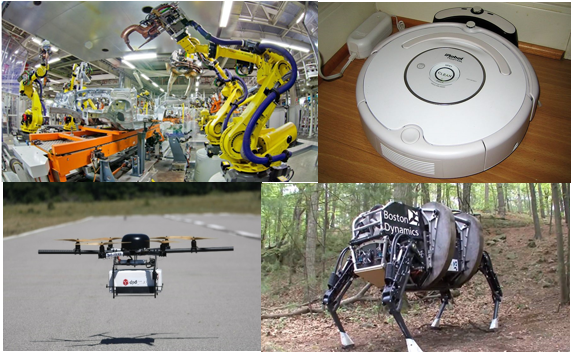
\includegraphics[width=0.8\textwidth]{figures/robots.png}
		\caption{Robots modernos}
		\label{fig.robots}
		\end{center}
\end{figure}

Hoy en día no solamente nos rodean los robots industriales, como los involucrados en cadenas de envasado de alimentos o cadenas de producción, sino que los robots cobran cada vez más importancia en entornos alternativos, como el doméstico entre otros, algunos de los cuales quedan representados en la Figura 1.1. Las aspiradoras robóticas (Roomba, Dyson, Xiaomi,…) han llegado a los hogares con éxito para realizar una tarea doméstica necesaria. Por otro lado, los vehículos de transporte aumentan cada vez más la tecnología robótica incorporada, como son los módulos de aparcamiento automático, u otros más avanzados como los asistentes de conducción autónoma (autopiloto de Tesla), o los recientes prototipos de coches autónomos que han lanzado grandes empresas como Google o Apple. Otros ámbitos, como el militar con máquinas capaces de desactivar bombas o realizar misiones de rescate, el de la medicina con el ejemplo del robot DaVinci que permite operar a un paciente desde cualquier parte del mundo con mayor precisión que la humana, o el de la logística en almacenes de Amazon tampoco están exentos de presencia robótica. Incluso se está trabajando para construir robots androides o humanoides capaces de desarrollar “comportamientos inteligentes” como el robot Asimo de Honda (Figura 1.2) o TOPIO, creado por TOSY Robotics (Figura 1.3), que puedan desempeñar tareas de interacción con herramientas y entornos humanos, ya sea con fines experimentales como el estudio de la locomoción bípeda, o incluso como auxiliar para la tercera edad o personas con movilidad reducida.

\begin{figure}[h]
	\centering
	\begin{minipage}[h]{.48\linewidth}
		\centering
		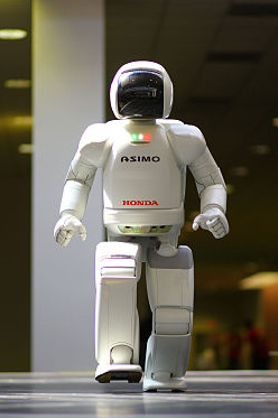
\includegraphics[width=.5\linewidth, height=7cm]{figures/asimo.png}
		\captionof{figure}{Robot Ásimo}
		\label{fig:asimo}
	\end{minipage}
	\begin{minipage}[h]{.48\linewidth}
		\centering
		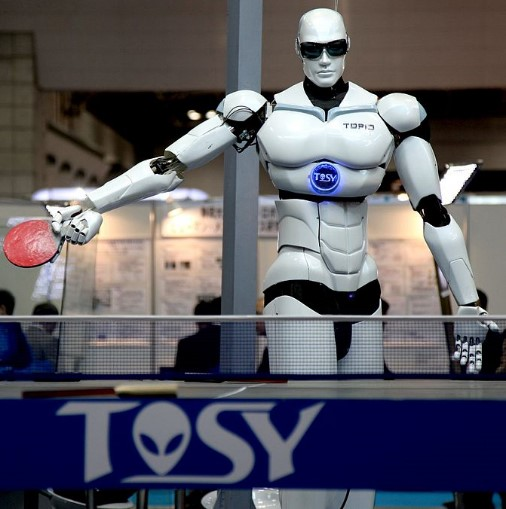
\includegraphics[width=.7\linewidth, height=7cm]{figures/topio.jpg}
		\captionof{figure}{Robot TOPIO}
		\label{fig:topio}
	\end{minipage}
\end{figure}

El abanico de aplicaciones que pueden involucrar sistemas robóticos es tan extenso como la imaginación de la comunidad dedicada a crearlos, por lo que tareas que nunca habíamos imaginado automatizadas son ahora labores totalmente robotizadas, como puede ser la agricultura de precisión a través de drones con análisis de imágenes térmicas y multiespectrales para aumentar el rendimiento de las explotaciones agrícolas, la automatización de aplicaciones anestésicas de bajo nivel e incluso competiciones deportivas de robots. 

Es difícil no parase a pensar en la potencia que tiene esta rama de la ciencia y la tecnología, y no sólo eso, sino también en la que puede alcanzar, ya que esto es sólamente el principio. En todo lo anterior, sale a relucir la utilidad de esta área de desarrollo, que permitirá en el futuro ganar en comodidad, economía e incluso salud. Es importante advertir la importancia de dominar esta disciplina en el futuro cercano, ya que será la llave que abrirá la puerta hacia un mundo más sencillo y seguro a través de la automatización.

\section{Software Robótico} 
Para la totalidad de los ejemplos mencionados es necesario que el comportamiento del software que controla dichos robots debe ser robusto. Es por eso que se divide en distintas capas (\textit{drivers}, \textit{middleware} y aplicaciones), cuya arquitectura es distinta según sea su aplicación final.

Lejos ya de ser controlados por personas, la mayoría de los robots están dotados de una autonomía que les permite desempeñar la tarea o tareas para las cuales han sido diseñados sin la mediación de terceros. Que dispongan de esta característica es posible gracias al minucioso desarrollo de sistemas complejos que constan de un software tal que compone algo parecido a una inteligencia autónoma.
El desarrollo de software robótico parte de ciertos requisitos o tareas, entre las que se incluyen circuitos de retroalimentación, filtrado de datos, control, búsqueda de caminos y localización entre muchas otras. 

En los últimos años han surgido numerosas plataformas de desarrollo de software para aplicaciones robóticas, también llamados \textit{middleware} robóticos. Los simuladores también son ingredientes habituales en el desarrollo de software robótico, permiten realizar las pruebas pertinentes, depurar los fallos programar una versión funcional del robot evitando el alto coste del proceso real una y otra vez. Estas herramientas son indispensables hoy en día para generar el conjunto de comandos codificados que indican al robot y a su sistema electrónico las acciones a realizar, así que entraremos un poco más en detalle en el siguiente apartado. Finalmente, las bibliotecas son de gran utilidad para generar el conjunto de comandos codificados que conforman el comportamiento del robot.

\subsection{Middlewares robóticos}
Los \textit{middleware} robóticos pueden definirse como entornos o \textit{frameworks} para el desarrollo de software para robots, es decir, software que conecta aplicaciones o componentes software para soportar aplicaciones complejas y distribuidas. Estos entornos suelen incluir \textit{drivers} para controlar los sensores y los actuadores de los robots, arquitectura software para las aplicaciones que se van a crear, bloques de funcionalidad robótica ya resuelta y otra serie de herramientas como simuladores, visualizadores… Es por eso que hay muchas reseñas del \textit{middleware} en las que se hace referencia a él bajo el nombre de “pegamento para software”. Una de las tareas de las que se encarga el middleware es de conectar nuestro hardware, real o simulado, con nuestra aplicación en desarrollo. El \textit{middleware} robótico más extendido en el mundo es ROS…

	\textbf{Robot Operating System (ROS)\footnote{\url{http://www.ros.org/}}}
	
Es una plataforma de software libre para el desarrollo de software de robots que provee la funcionalidad de un sistema operativo en un clúster heterogéneo, como el control de dispositivos de bajo nivel, la abstracción del hardware, el control de dispositivos de bajo nivel y mecanismos de intercambio de mensajes entre procesos, todos ellos de vital importancia para el desarrollo en este campo. Una de las razones que hace que ROS sea el \textit{framework} más utilizado es que, aunque se diseñó para ser utilizado principalmente en sistemas UNIX, se ha adaptado de forma que pueda utilizarse también en los otros sistemas operativos principales como Fedora, Debian,  Windows, MacOS X, Arch, Slackware, Gentoo u OpenSUSE, llegando incluso a abrir la puerta a la construcción de aplicaciones multiplataforma.

Existen algunos otros interesantes como: 

	\textbf{Orocos}\footnote{\url{http://www.orocos.org/}}
	
También encaja en el grupo de las plataformas de software libre para control avanzado de máquinas y robots basado en C++.
 
	\textbf{Orca}\footnote{\url{http://orca-robotics.sourceforge.net//}}
	
Un proyecto de software libre para aplicaciones de índole robótico que permite crear aplicaciones algo más complejas al estar orientado a componentes.

	\textbf{Urbi}\footnote{\url{https://github.com/urbiforge/urbi}}
	
\textit{Middleware} multiplataforma de código abierto en C++ que, utilizada de forma conjunta con ROS, permite desarrollar aplicaciones para sistemas complejos y completos.

	\textbf{JdeRobot}\footnote{\url{https://jderobot.org/}}
	
Plataforma para desarrollar aplicaciones robóticas y de visión artificial, que involucra nodos programados con varios lenguajes de programación y que es compatible con \textit{middlewares} de comunicaciones como ICE o ROS.

\subsection{Simuladores robóticos}
Generalmente, el diseño y puesta en escena de un robot es costoso y caro, por lo que no es aconsejable correr el riesgo de que el código implementado contenga errores que salgan a la luz en el momento de probarlo, ya que esto puede generar malfuncionamientos e incluso rotura del hardware. Es por eso que el paso previo a llevar el código a la máquina consiste en probarlo antes en un simulador orientado a este tipo de aplicaciones, lo que permite un desarrollo seguro y económico. Algunos de los simuladores más usados son:

	\textbf{Gazebo}\footnote{\url{http://gazebosim.org/}}
	
Es el simulador 3D de código abierto más distribuido, bajo licencia Apache 2.0. Destaca sobre los demás por sus motores de físicas, motor de renderizado avanzado y soporte para \textit{plugins} de robots y sensores, además de un amplio repertorio de robots comerciales y sus correspondientes sensores y actuadores. Además, se integra bien con ROS, permitiendo usar exactamente el mismo código de la simulación en el robot real.

	\textbf{Stage}\footnote{\url{http://wiki.ros.org/stage}}
	
Esta herramienta permite simular conjuntos numerosos de robots móviles en el plano bidimensional, integrable con ROS.

	\textbf{Webots}\footnote{\url{https://www.cyberbotics.com/}}
	
Simulador de robótica avanzada que permite definir modelos propios y su física, escribir controladores para ellos y hacer simulaciones a gran velocidad. Soporta el humanoide Nao. 

\subsection{Bibliotecas}
En el proceso de desarrollo de la parte software en robótica hay que resolver multitud de problemas clásicos y funcionalidades básicas además de las específicas para la aplicación en cuestión, ardua tarea para el programador que debe no sólo integrarlas en su proyecto, sino también abordarlas desde cero. Con el propósito de evitar esta situación, existen las bibliotecas, que no son más que conjuntos de implementaciones de código que ofrecen una interfaz bien definida para la funcionalidad que invocan. Su fin es ser utilizada por otros programas, independientes y de forma simultánea. Las bibliotecas pueden vincularse a un programa (o a otra biblioteca) en distintos puntos del desarrollo o la ejecución de dicho programa. Algunas de las bibliotecas utilizadas en robótica son: 
\begin{itemize}
	\item OpenCV \footnote{\url{https://opencv.org/}}: Es una biblioteca libre de visión artificial originalmente desarrollada por Intel. Contiene más de quinientas funciones que abarcan una gran gama de áreas en el proceso de visión, como reconocimiento de objetos, reconocimiento facial, calibración de cámaras, visión estéreo y visión robótica. Originalmente, OpenCV fue escrita en C++. Actualmente, la librería dispone de interfaces en C++, C, Python, Java y MATLAB. Es multiplataforma, existiendo versiones para GNU/Linux, Mac OSX, Windows y Android. 
 \item PCL \footnote{\url{http://pointclouds.org/}}: Se utiliza para el procesamiento digital de imágenes RGBD mediante el tratamiento de nubes de puntos 3D. Contiene numerosos algoritmos de última generación que incluyen filtrado, estimación de características, reconstrucción de superficies, ajuste de modelos y segmentación entre otros. Para simplificar el desarrollo, PCL se divide en una serie de bibliotecas de código más pequeñas, que se pueden compilar por separado. Es multiplataforma y ha sido compilada con éxito en Linux, Mac OSX, Windows y Android / iOS.
\end{itemize}

\section{Docencia en robótica}
La robótica con fines educativos está adquiriendo protagonismo estos últimos años en la enseñanza preuniversitaria, ya que proporciona un medio de aprendizaje para estudiantes de cualquier nivel, cuyo único requisito de partida es la motivación por el diseño de aplicaciones propias y su construcción. Con ello se consigue instruir a las personas en el campo de la robótica, pero no sólo eso, dado que para ello es necesario abordar temas multidisciplinarios (electrónica, informática, mecánica, física, etc.). El estudiante también adquiere conceptos de estas áreas científicas y tecnológicas. Además, proporciona una nueva visión del universo que le rodea, aprendiendo a distinguir los problemas  a su alrededor y a ser capaz de tomar una decisión al respecto.
La docencia en robótica en las etapas de enseñanza primaria y secundaria intenta despertar el interés de los estudiantes transformando las asignaturas tradicionales en más atractivas e integradoras, a la par que más prácticas, ya que crea entornos de aprendizaje propicios que recrean estos problemas que les rodean, y a través de los cuales pueden dar rienda suelta a su creatividad y plasmar en la realidad los conceptos teóricos que adquieren.
En los centros de enseñanza primaria y secundaria se imparte la robótica con frecuencia, mediante plataformas físicas como los robots LEGO (Mindstorms, RCX, NXT, Evo, WeDo), placas Arduino, los kits de SolidWorks, etc. 

\subsection{Docencia en la universidad}
En la docencia universitaria se imparten clases de robótica en ciertos Grados y Postgrados dentro de las escuelas de ingeniería. En España, podemos ver la robótica integrada en el “Grado en Ingeniería Robótica” de la Universidad de Alicante, y los Grados de “Electrónica industrial y automática” o en “Ingeniería Electrónica, Robótica y Mecatrónica” en diversas universidades, además de algunos otros que están por venir como el Grado en Ingeniería Robótica Software que habilitará la Universidad Rey Juan Carlos este próximo mes de Septiembre para el nuevo curso académico. Sin embargo, la enseñanza en robótica se concentra mayoritariamente en los programas de Postgrado, puesto que es una enseñanza más especializada. Existen Másteres destacados como el “Máster de Visión Artificial”, el “Máster Universitario en Ingeniería Mecatrónica”, o el “Máster Universitario en Automática y Robótica”.
Ya en el ámbito internacional se pueden destacar universidades especializadas en robótica como el MIT, Carnegie Mellon University, Stanford o Georgia Institute of Technology. Además, algunas asociaciones prestigiosas como ACM (Association for Computing and Machinery) y la IEEE-CS (IEEE Computer Society) ven la robótica como un área de conocimiento imprescindible en estudios de ingeniería, informática y sistemas inteligentes.
La Universidad Rey Juan Carlos cuenta con la plataforma de robótica JdeRobot, que posee un entorno académico conocido como JdeRobot-Academy, el cual es el contexto cercano de este trabajo. Este entorno educativo se ha empleado con éxito en diferentes asignaturas, como “Visión en Robótica” del Máster de Visión Artificial, o “Robótica” del Grado de Ingeniería Telemática. Asimismo, ha tenido éxito en cursos de introducción a la robótica y a la programación de drones.


\subsection{Entorno docente JdeRobot-Academy}
Los \textit{middleware} robóticos empleado para el desarrollo de este TFG son ROS y JdeRobot, que incluye el entorno académico JdeRobot-Academy\footnote{\url{https://jderobot.org/JdeRobot-Academy}}. Con este trabajo se ha pretendido extender sus posibilidades de aprendizaje, ampliándolo con dos nuevos ejercicios. 
\vspace{0.6cm}
Los ejes en los que se apoya JdeRobot-Academy son:
\begin{enumerate}[label=\alph*)]
	\item Lenguaje Python (por su sencillez y potencia),
	\item simulador Gazebo (con distintos modelos de robot, tales como drones, formula1, brazos, aspiradoras, etc.), y
	\item foco en el algoritmo en vez de en el middleware, ocultando al estudiante los detalles de la infraestructura.
\end{enumerate}

El entorno cuenta con un conjunto de prácticas, cada una de ellas enfocada a resolver un problema clásico de la robótica. Para cada práctica se ofrece un componente académico que resuelve tareas auxiliares como la interfaz gráfica, la conexión con sensores y actuadores concretos y la temporización entre otras, y  aloja el código del estudiante, que así se concentra en los algoritmos de percepción y control. Cada nodo está formado por una parte específica preparada, que queda oculta, y el código del estudiante, que simplemente rellena un sencillo fichero plantilla con la lógica del robot.

Se distinguen rápidamente varias capas de distinto nivel en su composición. Aunque la capa de nivel más bajo se da resuelta al alumno, queda de manifiesto que es necesario implementarla para dar soporte a cada práctica, incluyendo  la creación de los modelos del robot en el simulador y el escenario necesarios, los plugins que emplearán estos modelos como \textit{drivers}, y la comunicación entre el simulador y el componente académico de alto nivel. Todo ello se puede ver en la Figura 1.4: 

\begin{figure}[H]
  \begin{center}
    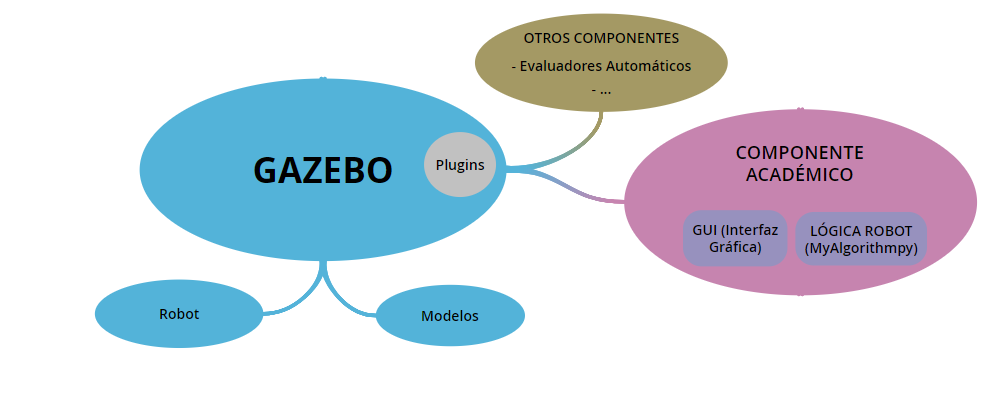
\includegraphics[width=0.9\linewidth]{figures/estructura_jde.png}
		\caption{Estructura de una práctica en JdeRobot-Academy}
		\label{fig.estructura}
		\end{center}
\end{figure}

En la Figura 1.4 se observa que los componentes académicos siguen una arquitectura software que facilita el desarrollo de las prácticas a los alumnos, los cuales únicamente deberán programar su algoritmo, ya sea el pilotaje en función de los datos que proporcionan los sensores o la planificación. Los componentes académicos cargan el código escrito por el alumno en el fichero plantilla llamado \textit{MyAlgorithm.py} (donde se materializa su resolución), y muestran en la interfaz  gráfica las pruebas o soluciones que realicen los alumnos, distintas trazas de depuración como pueden ser imágenes procesadas, datos láser, imágenes de cámaras integradas,…

Aunque el entorno suele emplear el simulador Gazebo, ha sido desarrollado para que el mismo código implementado en el fichero solución pueda ser ejecutado sobre un robot real. Es por eso que, con el driver adecuado, ese código puede operar un robot físico. El sistema operativo de base es Linux, para la cual se ha preparado la infraestructura. Adicionalmente, se ha puesto la vista en crear prácticas abordables desde otras plataformas, utilizado herramientas como la interfaz web de Gazebo, los cuadernillos de Jupyter (ver 3.6), tecnologías web de servidor y mediante el empleo de Dockers en vistas a disponer de una versión de la plataforma en MacOS y Windows.
Uno de los ejemplos de prácticas de los que dispone la plataforma es el ejercicio Color Filter que se muestra en la Figura 1.5:

\hspace{0.4\linewidth}
\textit{Color Filter}

\begin{figure}[H]
  \begin{center}
    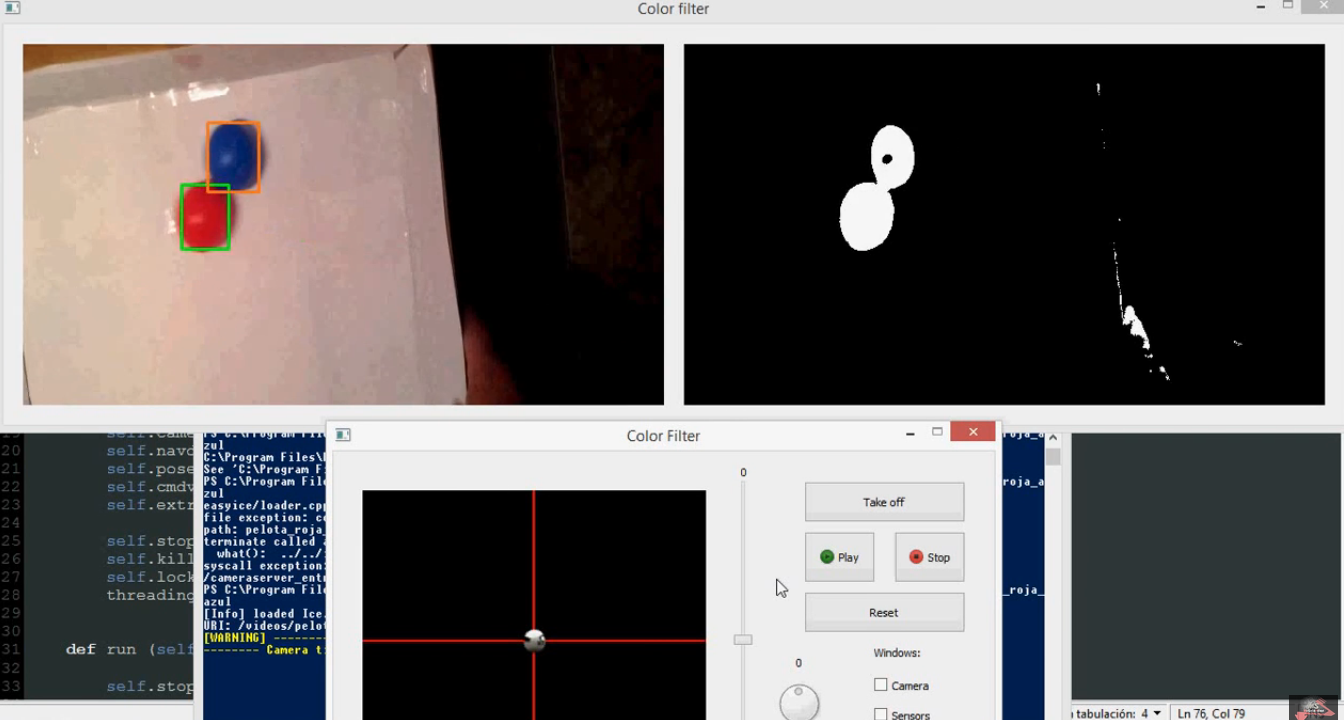
\includegraphics[width=0.95\textwidth]{figures/color_filter.png}
		\caption{Color Filter}
		\label{fig.colorfilter}
		\end{center}
\end{figure}

En este ejercicio el alumno puede experimentar con un filtro de color \footnote{\url{https://www.youtube.com/watch?v=tiXagRiqQnY}} aplicado sobre la secuencia de vídeo que proporciona un servidor de imágenes. Su código debe detectar el objeto relevante coloreado (pelotas rojas y azules) utilizando sendos filtros de color, y extraer su posición XY en las imágenes. 

\vspace{4cm}
\hspace{0.40\linewidth}
\textit{Bump\&Go}

\begin{figure}[H]
  \begin{center}
    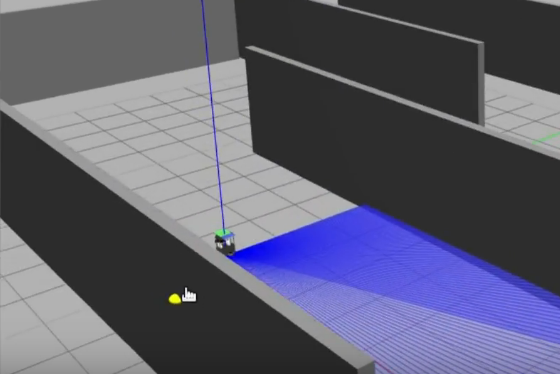
\includegraphics[width=0.50\linewidth, height=5cm]{figures/bumpngo.png}
		\caption{Bump{\&}Go}
		\label{fig.bumpgo}
		\end{center}
\end{figure}

El ejercicio \textit{Bump\&Go} (Figura 1.6) permite implementar una máquina de estados para controlar al robot kobuki en una simulación, un robot diseñado para ser duradero, resistente y rápido, que proporciona al programador acceso a sus motores y a sus sensores láser y de colisión. El alumno debe conseguir que el robot realice el comportamiento típico de chocar y girar\footnote{\url{http://jderobot.org/store/fperez/uploads/videos/bumpgoo.ogv}}.

\hspace{0.36\linewidth}
\textit{Labyrinth Escape}

\begin{figure}[H]
  \begin{center}
    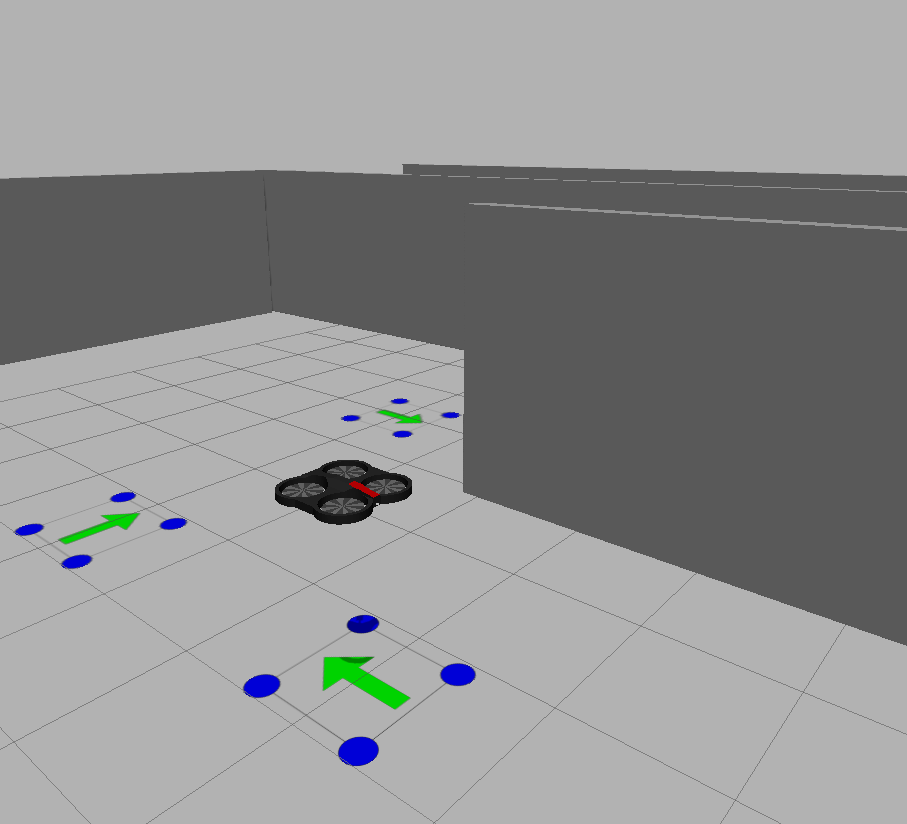
\includegraphics[width=0.50\linewidth, height=5cm]{figures/labyrinth_escape.png}
		\caption{Labyrinth Escape}
		\label{fig.laby}
		\end{center}
\end{figure}

En el ejercicio \textit{Labyrinth Escape} (Figura 1.7), el alumno debe programar la lógica de control de un dron con una cámara incorporada e interfaces de acceso a sus motores para lograr que salga con éxito de un laberinto a través de las imágenes que capta. Para ello, debe hacer uso de las herramientas de procesado y segmentación de imagen para reconocer e interpretar una serie de flechas verdes colocadas a lo largo del escenario que le indican el trazado que debe seguir para encontrar la salida\footnote{\url{https://youtu.be/EdWE5P3uZak}}.

\hspace{0.35\linewidth}
\textit{Obstacle Avoidance}

\begin{figure}[H]
  \begin{center}
    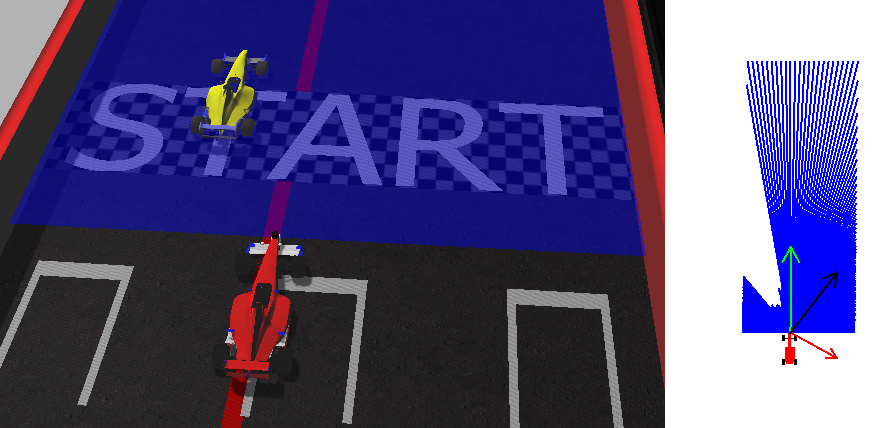
\includegraphics[width=0.95\textwidth, height=5cm]{figures/obstacle_avoidance.png}
		\caption{Obstacle Avoidance}
		\label{fig.obstacleavoidance}
		\end{center}
\end{figure}

En la práctica \textit{Obstacle Avoidance} el estudiante entra en contacto con la tecnología de coches autónomos (en este caso de tipo F1 como se puede ver en la Figura 1.8) equipado con un sensor láser y dos cámaras que ofrecen imágenes desde sus lados izquierdo y derecho. El alumno tendrá que hacer un uso inteligente de la información que el robot pone a su disposición en la simulación para construir una lógica de control y navegación local, la cual se encargará de seguir la carretera del circuito, tomar correctamente las curvas y esquivar los posibles obstáculos que vayan surgiendo en el camino\footnote{\url{https://youtu.be/gVvnrRDmLkI}}.

\vspace{7cm}
\hspace{0.35\linewidth}
\textit{Drone-Cat-Mouse}

\begin{figure}[H]
  \begin{center}
    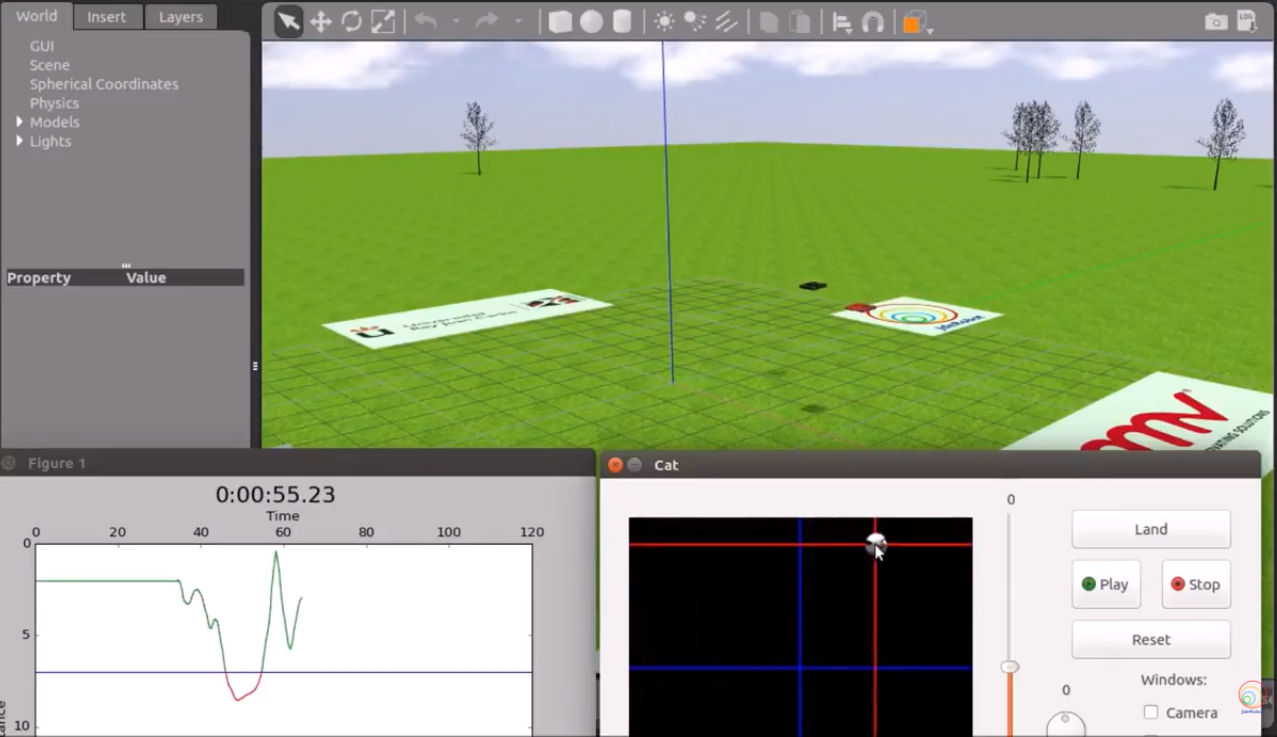
\includegraphics[width=0.95\textwidth, height=7.2cm]{figures/dronecatmouse.png}
		\caption{Drone-Cat-Mouse}
		\label{fig.dronecatmouse}
		\end{center}
\end{figure}

\textit{Drone-Cat-Mouse} es otra de las prácticas del entorno, en la que se ha de programar el dron negro para que persiga al dron rojo (pre-programado con diferentes niveles de dificultad) permaneciendo lo más cerca posible sin colisionar en un entorno simulado al aire libre, emulando el juego del gato y el ratón\footnote{\url{https://www.youtube.com/watch?v=DYD9oPawhWg}}. Esta práctica se  ha empleado en las dos ediciones previas del campeonato \textit{Program-A-Robot}, la primera en la URJC y la segunda en las Jornadas Nacionales de Robótica. Se va a emplear también en la tercera edición dentro de la conferencia internacional IROS\footnote{\url{https://www.iros2018.org/competitions}}.

\subsection{Ejercicios recientes}
El contexto inmediato de este trabajo de fin de grado reside en una serie de ejercicios elaborados recientemente también para ampliar las posibilidades de aprendizaje de JdeRobot-Academy. 

Entre ellos, cabe destacar el Trabajo de Fin de Grado de Irene Lope Rodríguez \textit{“Nuevas Prácticas en el Entorno Docente de Robótica JdeRobot-Academy”}\cite{tfg1}, que se centró en enriquecer la plataforma JdeRobot-Academy con dos nuevas prácticas llamadas ``Coche autónomo negociando un cruce'' y “Aspiradora autónoma con autolocalización”. La primera de ellas perseguía que un coche autónomo fuese capaz de reconocer una señal de STOP en un cruce vial a través de procesamiento de imágenes provenientes de tres cámaras a bordo del robot, desplegando el comportamiento habitual ante esta señal de detener el avance, examinar las vías perpendiculares para reconocer posibles coches circulando por ellas y, en caso de que las vías estén libres, girar a la derecha o izquierda para ocupar el carril correspondiente del sentido que se quiera seguir. La segunda de las prácticas que componían este trabajo tenía como objetivo reproducir el comportamiento de limpieza de un robot aspiradora de mercado, eliminado la suciedad en la mayor extensión posible del entorno en que se encuentra, el cual conoce a través de un mapa y un sensor de posición que le ubica en todo momento en la habitación simulada.

También hay que mencionar el Trabajo de Fin de Grado de Vanessa Fernández Martínez \textit{“Nuevas Prácticas en el Entorno Docente de Robótica JdeRobot-Academy”}\cite{tfg2}, en el que se añadió dos nuevas prácticas al repertorio de JdeRobot-Academy bajo los nombres de “Aspiradora autónoma” y “Aparcamiento automático”, además de mejorar la práctica ya existente \textit{“TeleTaxi”} con modelos mejorados, un mejor desempeño del algoritmo GPP de navegación global e incluso la inclusión de un evaluador automático capaz de medir el desempeño del algoritmo en función de distintos parámetros para proporcionar al alumno una nota final. En cuanto a los ejercicios creados, \textit{vacuum cleaner} se centró en un algoritmo de navegación sin localización basado en la serie 500 de aspiradoras \textit{Roomba} de iRobot, a través del cual debe recoger la suciedad de la mayor superficie posible de una casa. Por su parte, \textit{autopark} tiene como objetivo implementar un algoritmo basado en estados que permita a un coche autónomo realizar una maniobra de aparcamiento, reconociendo los huecos libres, evitando chocar y respetando los espacios de seguridad a través de los datos sensoriales del robot.

Continuando en esta línea de trabajo, el presente TFG se apoya en la filosofía de estos dos trabajos precedentes para aportar a JdeRobot-Academy dos prácticas que involucren elementos hasta ahora no presentes en las demás: una empleando hardware real y otra haciendo uso de \textit{drivers} de ROS directos.

\vspace{3cm}

El objetivo general de este TFG es ampliar las posibilidades de esta plataforma docente, creando nuevas prácticas y mejorando las ya existentes, aumentando su versatilidad. En los próximos capítulos abordaremos todos los elementos necesarios para conseguir este objetivo, empezando por el Capítulo 2, en el que concretaremos los objetivos que se han marcado, así como los requisitos de partida y la metodología empleada. En el Capítulo 3 se expondrá la infraestructura utilizada para llevar a cabo el proyecto. En los Capítulos 4 y 5 se abordarán las prácticas que se han creado. Por último, en el Capítulo 6 se expondrán las conclusiones obtenidas, así como las posibles líneas de mejora que se pueden seguir.
\lhead[]{CAP\'ITULO \thechapter. OBJETIVOS}
\chapter{Objetivos}\label{cap.objetivos}
En este punto ya hemos introducido el contexto en el que desarrolla el trabajo, es momento de describir los objetivos que se han tratado de alcanzar, los requisitos para las soluciones desarrolladas y la metodología seguida para su consecución.

\section{Objetivos}
La meta de este proyecto consiste en la creación de dos nuevas prácticas de sistemas robóticos para el entorno docente JdeRobot-Academy, una primera que consistirá en seguimiento de caras a través de una cámara y otra sobre auto localización de un robot basada en láser. Para cada una de ellas se creará la infraestructura necesaria y una solución de referencia.

En primer lugar, la práctica de seguimiento de caras utilicará una cámara móvil montada en un cuello mecánico, la cual puede apuntarse hacia varias direcciones, para que el alumno ponga en práctica sus conocimientos de segmentación de imagen buscando posibles caras de personas en la imágenes que le sirve dicha cámara, y generando órdenes para los motores de la cámara de modo que esta siga con la mirada el movimiento de la persona que tiene delante.

La segunda práctica creada es sobre un robot móvil y busca resolver un problema de auto localización basada en láser, de manera que dicho robot sepa en todo momento su posición y orientación en el entorno que le rodea, valiéndose únicamente de un sensor láser incorporado.

\section{Requisitos} 
El software desarrollado, además de proporcionar las dos prácticas deseadas, deberá cumplir estos requisitos de partida del proyecto:

\begin{enumerate}
	\item El sistema operativo que se empleará para este proyecto será Ubuntu 16.04 LTS.
	\item Se hará uso del middleware robótico JdeRobot en su versión 5.6.1. El uso de esta plataforma simplifica el desarrollo del comportamiento del robot.
	\item Se hará uso de OpenCV3 en la práctica de seguimiento de caras.
	\item En el ejercicio de localización basada en láser se usará \textit{ROS-Kinetic} y todas las simulaciones se realizarán en el simulador Gazebo, en concreto en la versión 7.9.0. 
	\item El lenguaje de desarrollo empleado para crear los distintos componentes será Python, en concreto en su versión 2.7.12. Por compatibilidad con JdeRobot-5.6.1 y de éste con el middleware ROS \textit{Kinetic} no se ha usado Python-3.x
	\item Las soluciones han de ejecutar algoritmos que funcionen en tiempo real, de manera que deberán ser eficientes y ejecutar movimientos suaves.
\end{enumerate}

\section{Metodología}
La elaboración de este trabajo podría descomponerse en un conjunto de iteraciones con varias fases, en cada una de las cuales se establecía una reunión con el tutor para determinar los subobjetivos siguientes, planificar cómo abordarlos, analizar los posibles problemas y corregir fallos. Así, se ha conseguido un desarrollo fluido y completo, asentando los conocimientos y despejando las dudas que surgían a lo largo de los meses que se dedicó al trabajo.

Parte del seguimiento lo hemos hecho utilizando herramientas de apoyo, como la bitácora semanal en la Wiki de JdeRobot \footnote{\url{https://jderobot.org/Cawadallah-tfg}} donde periódicamente se redactaban los avances realizados y se añadían vídeos demostrativos de lo conseguido, imágenes representativas y texto descriptivo. El código asociado a los avances se almacenó en un repositorio personal de GitHub\footnote{\url{https://github.com/cawadall/Academy}}\footnote{\url{https://github.com/cawadall/JdeRobot}}, al que el tutor ha podido acceder en todo momento para aportar realimentación y favorecer el progreso.

Se ha optado por seguir el modelo de desarrollo en espiral creado por Barry Boehm, el cual hemos creído que se adaptaba perfectamente a nuestras necesidades, permitiéndonos separar el comportamiento final en varias sub-tareas más sencillas, a la par que disponer de flexibilidad ante cambios en los requisitos, algo bastante común a medida que avanzaba el desarrollo. Con él, conseguimos una resolución temprana de riesgos y poder definir la arquitectura en las fases iniciales, todo ello basado en un proceso continuo de verificación de la calidad.

\begin{figure}[H]
  \begin{center}
    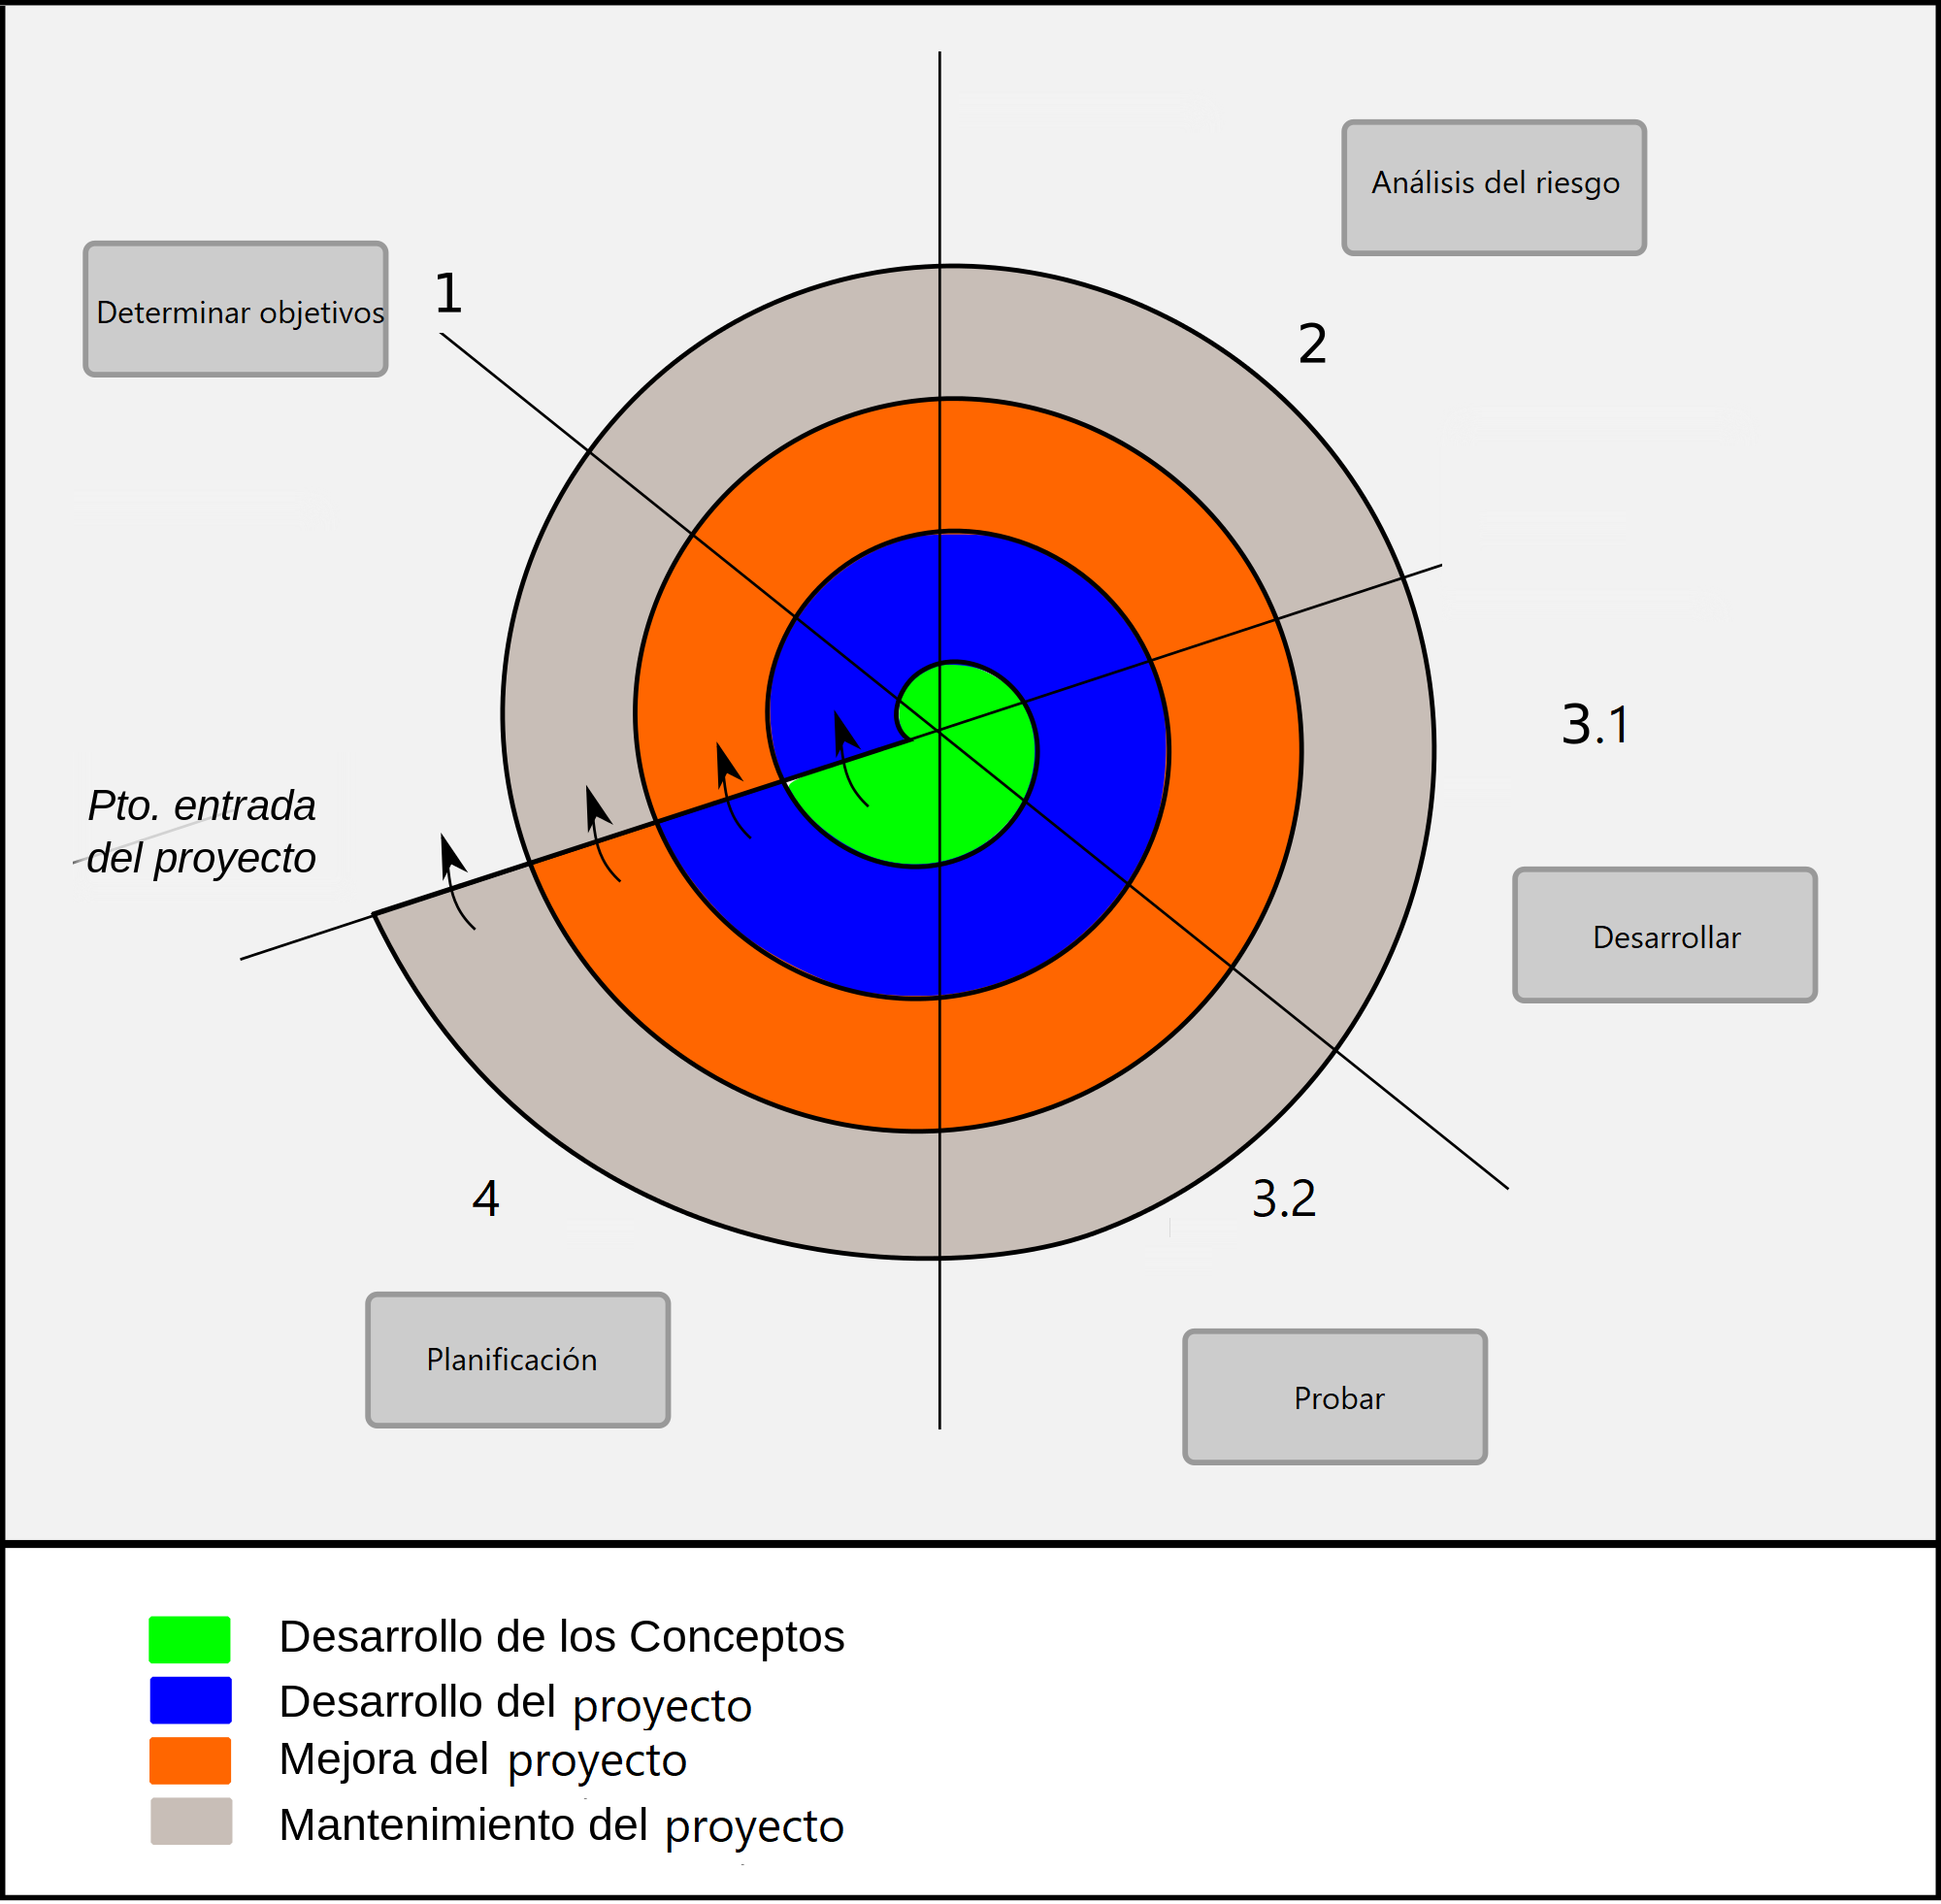
\includegraphics[width=0.9\linewidth]{figures/modelo_espiral.png}
		\caption{Modelo de desarrollo en espiral}
		\label{fig.espiral}
		\end{center}
\end{figure}

Como se puede ver en la Figura 2.1, este modelo de ciclo de vida permite ir obteniendo prototipos funcionales en primera instancia, luego mejorar el prototipo conseguido y, por último, pulir los detalles para cubrir todos los requisitos.  Así, se realiza el trabajo de forma incremental, en forma de ciclos con cuatro fases bien definidas:

\begin{itemize}
	\item[--] \textbf{Determinar objetivos}: en esta primera fase del ciclo se definen las metas que se deben conseguir para que una vez completadas se pueda dar por finalizado el mismo.
	\item[--] \textbf{Análisis del riesgo}: en la segunda fase se evalúa qué problemas es posible encontrarse al empezar el desarrollo, y se piensa en cómo abordarlos.
	\item[--] \textbf{Desarrollar y probar}: en la tercera fase es en la que, tras evaluar los riesgos, se procede al propio desarrollo del trabajo, además de las correspondientes pruebas para verificar su correcta funcionalidad.
	\item[--] \textbf{Planificación}: en esta última fase se valoran los resultados obtenidos en el ciclo y se planifican las siguientes etapas del proyecto.
\end{itemize}

\section{Plan de trabajo}
Para lograr los objetivos descritos, se han seguido las siguientes etapas de trabajo:

\begin{itemize}
	\item[--] \textbf{Familiarización con el entorno JdeRobot}. Tras la descarga e instalación del software  involucrado, incluyendo dependencias, simulador y bibliotecas necesarias, se tratará de entrar en contacto con el entorno JdeRobot modificando y pulimentando algunas prácticas existentes para añadir mejoras, por ejemplo, en sus interfaces gráficas.
	\item[--] \textbf{Toma de contacto con el simulador Gazebo}. En esta etapa se han estudiado distintos ejemplos disponibles en la web de Gazebo\footnote{\url{http://gazebosim.org/tutorials}} y de JdeRobot. Además, se ha estudiado el funcionamiento básico de los \textit{plugins}  que Gazebo emplea para controlar los robots, sus sensores y sus actuadores. Esto ha implicado la investigación del lenguaje de programación C++, el cual también ayudará a comprender los \textit{plugins} ROS.
	\item[--] \textbf{Estudiar las bibliotecas involucradas}, entre las cuales destacan OpenCV, Threading, NumPy y PyQt5.
\end{itemize}

Una vez aquí, se centrarán los esfuerzos en…

\begin{itemize}
	\item[--] \textbf{Desarrollo de la infraestructura para la práctica de seguimiento de caras}. Manejo de los \textit{drivers} involucrados para el control de los motores y de la cámara. Se creará el nodo académico que albergará el código del estudiante. También se creará una versión de la práctica a través de Jupyter.
	\item[--] \textbf{Programación de una solución de referencia para el seguimiento de caras}.
	\item[--] \textbf{Preparación de la infraestructura para el ejercicio de autolocalización basada en láser}. Se desarrollará el \textit{driver} para el robot simulado. Se creará el nodo académico que alberga el código del estudiante, además de un cuadernillo de Jupyter con la misma funcionalidad.
que alberga alternativamente el código del estudiante.
	\item[--] \textbf{Programación de una solución de referencia para la autolocalización}.
	\item[--] \textbf{Obtención de conclusiones} acerca de lo estudiado, con las cuáles completar la formación en el campo.
\end{itemize}
\lhead[]{CAP\'ITULO \thechapter. INFRAESTRUCTURA}
\chapter{Infraestructura}\label{cap.infraestructura}
Este capítulo se ocupa de detallar  los componentes y piezas software existentes en las que nos hemos apoyado en el desarrollo del trabajo. Profundizaremos en las plataformas sobre las que se apoya el trabajo (ROS y JdeRobot), en la simulación de las acciones del robot que realiza Gazebo, en las librerías de mayor importancia (OpenCV para la primera práctica y PyQt para las interfaces gráficas) y, por último, en el proyecto Jupyter.

\section{Simulador Gazebo}
Gazebo\footnote{\url{http://gazebosim.org/}} es un simulador usado en robótica que permite emular diversos escenarios tridimensionales para robots autónomos (\textbf{Figura 3.2}). Es particularmente adecuado para probar algoritmos de elusión de objetos y de visión artificial. Cuando se trata de escribir el código que controlará un robot, especialmente si se está aprendiendo, es necesario realizar pruebas con el software, las cuales pueden ser muy costosas de implementarse en hardware real. Por ello, usamos simuladores que nos permitan comprobar en hardware virtual el comportamiento de nuestra lógica en todo momento, agilizando el desarrollo y abaratando costes. 

El simulador utilizado en este TFG será Gazebo, el cual es de código abierto. Por su versatilidad (es capaz de simular robots, objetos y sensores en entornos complejos de interior y exterior), su interfaz de gran calidad, y su robusto motor de físicas (para describir componentes como la masa del robot, rozamiento, inercia, amortiguamiento, etc.), fue elegido para realizar el DARPA Robotics Challenge (2012–2015) y está mantenido por la Fundación Open Robotics\footnote{\url{https://www.openrobotics.org/}}.

\begin{figure}[H]
  \begin{center}
    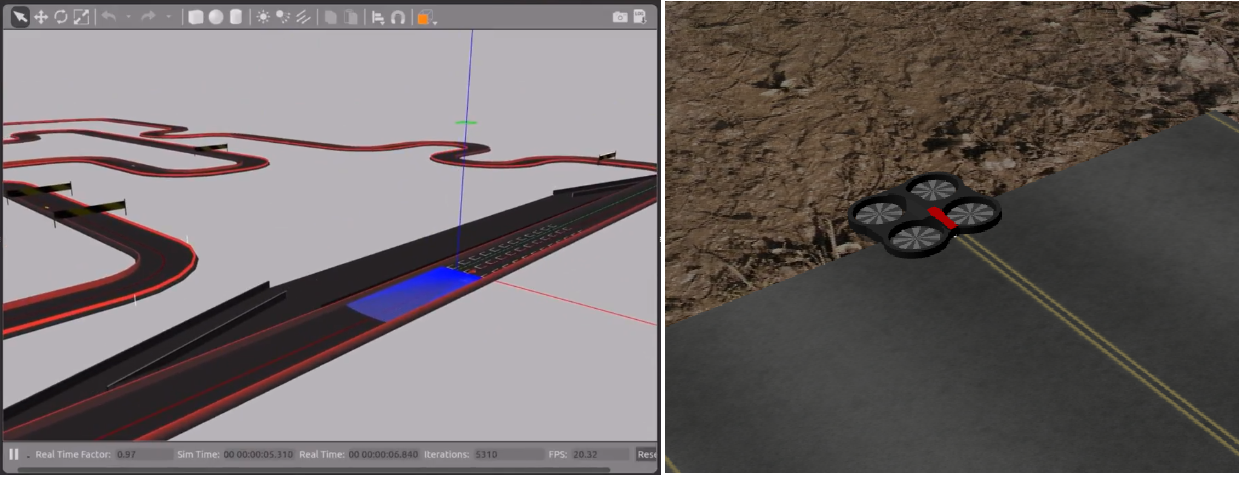
\includegraphics[width=0.9\linewidth]{figures/gazeboworlds.png}
		\caption{Ejemplo de mundo y modelo de Gazebo}
		\label{fig.worlds}
		\end{center}
\end{figure}

Los mundos 3D simulados con Gazebo se describen en ficheros con extensión “.world”, que no son más que ficheros XML (Extensible Markup Language) de descripción de documentos, definidos en el lenguaje Simulation Description Format (SDF), donde se recogen todos los elementos del escenario:

\begin{itemize}
	\item Escena: Luz ambiente, propiedades del cielo, sombras, etc.
	\item Mundo: Representa el mundo como un conjunto de modelos, \textit{plugins} y propiedades físicas.
	\item Modelo: Articulaciones, objetos de colisión, sensores, etc.
	\item Físicas: Gravedad, motor físico, paso del tiempo, colisiones, inercias, etc.
	\item \textit{Plugins}: Sobre un mundo, modelo o sensor. Pueden crearse o utilizarse los disponibles en la red como \textit{libroombaplugin.so}, que da acceso y control sobre todas las interfaces de un cierto modelo de robot.
\end{itemize}

Todos y cada uno de ellos cuentan con una etiqueta propia. Los modelos de robots que se emplean en la simulación son creados mediante programas de diseño y modelado 3D como Blender o Sketchup. En la versión 7 de Gazebo se ha incorporado un editor de modelos muy básico con el que se pueden crear robots y mundos básicos. A partir del modelo, se ha de asociar un \textit{plugin} al mismo para recoger y publicar la información de los sensores, y para acceder a los actuadores y dotar al robot de inteligencia e interacción.

\section{Entorno ROS}
ROS (Robot Operating System) proporciona bibliotecas y herramientas para ayudar a los desarrolladores de software a crear aplicaciones de robots. Proporciona abstracción de hardware, controladores de dispositivo, bibliotecas, visualizadores, intercambio de mensajes y administración de paquetes entre otras cosas. Se distribuye bajo una licencia BSD de código abierto.

Uno de sus puntos fuertes es su integración con el simulador Gazebo a través de una serie de paquetes llamados \textit{gazebo\_ros\_pkgs}\footnote{\url{http://ros.org/wiki/gazebo\_ros\_pkgs}} que proporcionan las interfaces necesarias para simular un robot en Gazebo usando \textit{ROS Messages}, servicios y reconfiguración dinámica.

Este entorno se basa en la representación del modelo de un robot a través de nodos, procesos que conllevan computación. Los nodos se combinan en un gráfico y se comunican entre sí mediante \textit{topics} de transmisión, servicios RPC y el Servidor de Parámetros. Un sistema de control de un robot generalmente comprenderá muchos nodos, por ejemplo, un nodo controla un láser de largo alcance, otro nodo controla los motores de las ruedas del robot, otro se encarga de la localización, se usa otro nodo para la planificación de rutas, un nuevo nodo proporciona una vista gráfica del sistema, y así sucesivamente. El uso de nodos en ROS proporciona varios beneficios para el sistema en general. Hay tolerancia adicional a fallos ya que los problemas están aislados en nodos individuales. La complejidad del código se reduce en comparación con los sistemas monolíticos.

En cuanto a los \textit{topics} como forma de comunicación, se definen como buses sobre los cuales los nodos intercambian mensajes. Los \textit{topics} tienen una semántica de publicación y/o suscripción anónima, que desacopla la producción de información de su consumo. En general, los nodos no saben con quién o quiénes se están comunicando. En cambio, los nodos que están interesados en ciertos datos se suscriben al \textit{topic} relevante y por su parte aquellos nodos que generan datos de cierto tipo los publicarán en el \textit{topic} correspondiente. Puede haber varios editores y suscriptores de un \textit{topic}.

Dada la compatibilidad entre el entorno ROS, el simulador Gazebo y la plataforma JdeRobot, se puede hacer uso de \textit{plugins} de ROS para las simulaciones que se comunicarán con el nodo académico de las prácticas a través de \textit{topics}, por los que circulará información con el formato correspondiente. Existe una gran variedad de \textit{drivers} en la red para controlar las interfaces de muchos modelos, sensores y actuadores. Entre ellos, el \textit{driver usb\_cam} permite interactuar con cámaras USB estándar (por ejemplo, SonyEvi d100p o Logitech Quickcam) utilizando libusb\_cam\footnote{\url{https://github.com/libusb/libusb/wiki}}, una biblioteca multiplataforma para acceso genérico a dispositivos USB, y publica imágenes bajo el formato de mensajes \textit{sensor\_msgs::Image}\footnote{\url{http://docs.ros.org/api/sensor\_msgs/html/msg/Image.html}} 
 de ROS. Además, utiliza la biblioteca \textit{image\_transport}\footnote{\url{http://wiki.ros.org/image\_transport}} para permitir el transporte de imágenes comprimidas. A través de él obtendremos las imágenes que proporciona la cámara en la primera de las prácticas que se va a crear. Otros ejemplos son \textit{libgazebo\_ros\_laser} o \textit{libgazebo\_ros\_diff\_drive} pueden utilizarse para controlar las interfaces láser y motores respectivamente en un robot simulado.

\section{Entorno JdeRobot}
JdeRobot\footnote{\url{https://jderobot.org/}} es un \textit{middleware} abierto para el desarrollo de aplicaciones con robots y visión artificial. Esta plataforma fue creada por el Grupo de Robótica de la Universidad Rey Juan Carlos en 2003 y está licenciada como GPLv3\footnote{\url{https://www.gnu.org/licenses/quick-guide-gplv3.html}}.
Su estructura ha sido desarrollada en C y C++, aunque algunas de sus componentes están escritas Python y JavaScript. El entorno que ofrece está basado en componentes, los cuales se ejecutan como procesos. Dichos componentes interoperan entre sí a través de \textit{middlewares} de comunicaciones ICE o  ROS, según sea la aplicación. Tanto ICE como \textit{ROS-Messages} permiten la interoperación entre los componentes incluso estando desarrollados en diferentes lenguajes.

La plataforma facilita los \textit{drivers} necesarios para poner en marcha los modelos disponibles. Estos \textit{drivers} están asociados a un dispositivo hardware del robot, ya sea sensor o actuador, e incluyen el correspondiente interfaz para acceder a él. Esto simplifica el acceso desde las aplicaciones a los diferentes componentes hardware, ya que con una simple función se puede enviar o recibir datos de ellos a través de interfaces ICE o ROS.

JdeRobot ofrece soporte a una amplia gama de dispositivos entre los que podemos encontrar cuadricópteros (AR Drone de Parrot), el robot Kobuki de Yujin Robot, el humanoide NAO de Aldebaran Robotics, cámaras firewire, USB e IP, los escáneres laser LMS de SICK y URG de Hokuyo, los simuladores Stage y Gazebo, sensores de profundidad como Kinect y otros dispositivos X10 de domótica. 

También incluye \textit{drivers} específicos para solucionar aspectos de control de cámaras y drones entre otros. Destaca para este trabajo el \textit{driver EVIcam}, de utilidad para la primera de las prácticas que se va a incluir en el entorno, que ha sido desarrollado e incluido en la plataforma JdeRobot para poder teleoperar cámaras vía software a través de una conexión USB. En concreto, utiliza una interfaz ICE para poder controlarla a través de comandos de movimiento. 
El código fuente puede encontrarse en: 

\url{https://github.com/JdeRobot/JdeRobot/tree/master/src/drivers/evicam_driver}

En las aplicaciones en JdeRobot se utilizan bibliotecas de software libre que son estándares de facto en su campo como OpenCV para visión, PCL para manejo de nubes de puntos o Eigen para álgebra. JdeRobot es compatible con ROS, en particular con la versión ROS-Kinetic, por lo que las aplicaciones pueden incorporar fluidamente nodos de ROS y conectarse a ellos.

Las prácticas que componen este trabajo se harán a través de la versión 5.6.1, última versión estable de la misma.

\section{Lenguaje Python}
Python\footnote{\url{https://www.python.org/}} es un lenguaje de programación interpretado, orientado a objetos y de alto nivel con semántica dinámica. Suele destacar por su apariencia intuitiva, resultando en un lenguaje fácil de aprender. Su creador fue Guido van Rossum, un investigador holandés que trabajaba en el centro de investigación CWI (Centrum Wiskunde \& Informatica). La primera versión surgió en 1991 pero no fue publicado hasta tres años después. Guido dio el nombre de Python a su lenguaje en honor a la serie de televisión \textit{Monty Python’s Flying Circus}.

Sus estructuras de datos integradas de alto nivel, combinadas con el tipado dinámico y el enlace dinámico, lo hacen muy atractivo para el desarrollo rápido de aplicaciones, así como también para usarlo como scripting o lenguaje para conectar componentes existentes. La sintaxis simple y fácil de aprender de Python enfatiza la legibilidad y, por lo tanto, reduce el costo del mantenimiento del programa. Python admite módulos y paquetes, lo que fomenta la modularidad del programa y la reutilización de código. 

El intérprete de Python y la extensa biblioteca estándar están disponibles en formato fuente o binario sin cargo para las plataformas principales, y se pueden distribuir libremente.

La última versión ofrecida por Python Software Foundation, su administrador, es la 3.6.5. En este TFG vamos a emplear el lenguaje en su versión 2.7.12 junto con JdeRobot 5.6.1, que a su vez utiliza dicha versión por compatibilidad con ROS Kinetic. Usaremos este lenguaje para programar tanto los nodos académicos como las soluciones de referencia.

\section{Biblioteca OpenCV}
OpenCV\footnote{\url{https://opencv.org/}} es una librería de código abierto desarrollada inicialmente por Intel y publicada bajo licencia de BSD. Esta librería implementa gran variedad de herramientas para el procesado de imagen y el aprendizaje máquina. Sus siglas provienen del inglés, y significan \textit{“Open Source Computer Vision Library”}. Su propósito es facilitar la programación de aplicaciones de visión por computador en tiempo real.

Esta librería puede ser usada en MacOS, Windows, Android y Linux, y existen versiones para C\#, Python y Java, a pesar de que originalmente era una librería en C/C++. Además, hay interfaces en desarrollo para Ruby, Matlab y otros lenguajes.
OpenCV principalmente implementa algoritmos para las técnicas de calibración, detección de rasgos, seguimiento de caras, rastreo de objetos, análisis de la forma, análisis del movimiento, reconstrucción 3D, segmentación de objetos, reconocimiento, clasificación de acciones humanas en vídeos,…  Los algoritmos se basan en estructuras de datos flexibles acopladas con estructuras IPL (\textit{Intel Image Processing Library}), aprovechándose de la arquitectura de Intel en la optimización de la mayoría del paquete.
Fue diseñado para tener una alta eficiencia computacional. Está escrito en C y puede aprovechar las ventajas de los procesadores \textit{multicore}. Tantas son las ventajas y las posibilidades grandes compañías como Google, Yahoo, Microsoft, Intel, IBM, Sony, Honda o Toyota emplean la librería, que se ha convertido en el estándar de facto en el campo. 

En este trabajo se ha empleado la versión 3.2 de OpenCV en Python. Esta librería se empleará para todo lo relacionado con el tratamiento de imágenes (análisis y procesado). 

\section{Biblioteca PyQt}
PyQt\footnote{\url{https://pypi.org/project/PyQt5/}} es un conjunto de enlaces Python para el conjunto de herramientas Qt, un \textit{framework} multiplataforma orientado a objetos en C++  que permite desarrollar interfaces gráficas e incluye sockets, hilos, Unicode, bases de datos SQL, etc. PyQt combina todas las ventajas de Qt y Python, permite emplear todas las funcionalidades ofrecidas por Qt con un lenguaje de programación tan sencillo como Python. Fue desarrollado por Riverbank Computing Ltd y es soportado por Windows, Linux, Mac OS/X, iOS y Android.

En este proyecto se ha empleado la versión 5 de PyQt. PyQt5 es un conjunto de enlaces Python para Qt5, disponible en Python 2.x y 3.x. Tiene más de 620 clases y 6000 funciones y métodos. PyQt5 dispone de una licencia dual, es decir, los desarrolladores pueden elegir entre una licencia GPL (General Public Licence) o una licencia comercial. 
Las clases de PyQt5 se dividen en ciertos módulos, tales como QtCore, QtGui, QtWidgets, QtXml o QtSql. En las prácticas desarrolladas se ha hecho uso de los siguientes módulos para implementar las interfaces de usuario:

\begin{itemize}
	\item QtCore: contiene las funcionalidades principales no relacionadas con la interfaz gráfica. Este módulo se emplea para trabajar con archivos, diferentes tipos de datos, hilos, procesos, url, etc.
	\item QtGui: contiene clases para el desarrollo de ventanas, gráficos 2D, imágenes y texto.
	\item QtWidgets: dispone de clases que proporcionan un conjunto de elementos de interfaz de usuario para crear interfaces de usuario clásicas de escritorio. 
\end{itemize}

\section{IPython 3.0 - Jupyter}
Jupyter Notebook\footnote{\url{http://jupyter.org/}} es una aplicación web de código abierto que permite al usuario crear y compartir documentos que contengan códigos empotrados, ecuaciones, visualizaciones y textos narrativos. Entre sus usos destacan: limpieza y transformación de datos, simulación numérica, modelado estadístico, visualización de datos, aprendizaje automático, aunque su funcionalidad es mucho mayor. Jupyter es el nombre que desde hace poco se usa para referirse a IPython 3.0.

La herramienta principal de la aplicación son sus cuadernillos (\textit{Notebooks}), que son los documentos producidos por Jupyter Notebook que contienen código de computadora (por ejemplo, Python), elementos de texto enriquecido (párrafos, ecuaciones, figuras, enlaces, etc.) y demás. Los documentos del cuaderno son documentos legibles por humanos que contienen la descripción del análisis y los resultados (figuras, tablas, etc.) así como documentos ejecutables para realizar análisis de datos.
Los \textit{Notebooks} consisten en una secuencia lineal de celdas. Hay cuatro tipos básicos:

\begin{itemize}
	\item \textbf{Celdas de código}: entrada y salida del código en vivo que se ejecuta en el kernel. 
	\item \textbf{Casillas de reducción}: texto narrativo con ecuaciones LaTeX incrustadas.
	\item \textbf{Encabezado de celdas}: 6 niveles de organización jerárquica y formato.
	\item \textbf{Celdas sin formato}: texto sin formato que se incluye, sin modificaciones, cuando los cuadernillos se convierten a diferentes formatos mediante \textit{nbconvert}.
\end{itemize}

Así, la aplicación servidor-cliente permite editar y ejecutar estos \textit{Notebooks} a través de un navegador web. La aplicación Jupyter Notebook se puede ejecutar en un escritorio local que no requiere acceso a Internet o puede instalarse en un servidor remoto y acceder a ella a través de Internet. Además de mostrar, editar y ejecutar documentos, la aplicación tiene un \textit{Dashboard} (Panel de instrumentos del cuadernillo), que es similar a un ``panel de control'' que muestra los archivos locales y permite abrir documentos del cuaderno o cerrar sus núcleos (\textit{kernels}). 

Estos \textit{kernels} son ``motores computacionales'' que ejecutan el código contenido en un \textit{Notebook} (el núcleo IPython ejecuta el código Python). Existen núcleos o \textit{kernels} oficiales para muchos lenguajes (Python, Julia, R, Ruby Haskell, Scala,…), e incluso versiones distintas de un mismo lenguaje de programación. Cuando se abre un \textit{Notebook}, el \textit{kernel} asociado se inicia automáticamente, de manera que al ejecutar cada celdilla con código, realiza el cálculo y produce los resultados.  Dependiendo del tipo de cálculos, el \textit{kernel} puede consumir CPU y RAM significativas, pudiendo ejecutar procesos más exigentes. 

Estos documentos pueden ser salvados y almacenados en el sistema de ficheros local, como un documento con extensión \textit{.ipynb}, para ser ejecutado cuando se quiera. Esto nos permitirá realizar una versión análoga a la que se hará en JdeRobot a través de Jupyter, con el código de la práctica empotrado, widgets interactivos y una pequeña guía para el alumno. Los \textit{Notebooks} que haremos se basarán en código Python versión 2.7. 
\lhead[]{CAP\'ITULO \thechapter. FOLLOW FACE}
\chapter{Práctica 1: Detección y seguimiento de caras con Sony Evi d100p}\label{cap.followface}
En este punto ya se han presentado contexto, los objetivos y las herramientas empleadas para llevar a cabo este proyecto, de manera que este capítulo está reservado para detallar el proceso de realización de la primera de las dos prácticas creadas en y para el entorno JdeRobot. Se explicará la infraestructura que le da soporte, el hardware involucrado y su forma de comunicación e interacción, el componente académico y la solución de referencia.

\section{Enunciado} \label{sec.enunciado}
Ésta práctica persigue que una cámara real sea capaz de seguir caras de personas. La cámara, evidentemente, sólo proporcionará sus imágenes captadas, a través de una capturadora de vídeo que irá proporcionando al nodo académico los frames  sucesivos. Además, la cámara dispondrá de dos actuadores de movimiento que controlarán su movimiento horizontal y vertical, a los cuales a partir de ahora llamaremos \textit{Pan} y \textit{Tilt} respectivamente.

Con todo ello, el alumno deberá programar un algoritmo de segmentación de caras de personas en la imagen y de control gradual en base a los datos que proporciona la imagen segmentada. Para ello, hay disponibles distintos elementos de \textit{debugging} o corrección de errores en el interfaz gráfico (GUI), ya que incluye espacios para la visualización de la imagen captada por la cámara y de la imagen segmentada, accesibles con dos sencillos objetos Python.

El algoritmo responde a un control reactivo, que en cada instante actuará en función de los datos de los sensores y sus propias variables internas. El control reactivo permitirá establecer en todo momento el movimiento del robot y responder ante situaciones imprevistas.

\section{Infraestructura}
En este apartado se introducirán los distintos componentes sobre los que se apoya la práctica, principalmente del hardware empleado y sus drivers controladores, pero también el componente académico, la interfaz y el código auxiliar.

\subsection{Cámara Sony Evi d100p}
El robot utilizado en esta práctica será la cámara Sony Evi modelo d100p, como el que se muestra en la Figura inferior (\textbf{Figura 4.1}), de la multinacional japonesa especializada en electrónica, \textit{gaming} y entretenimiento.

Este modelo cuenta con las siguientes características:
\begin{multicols}{2}
\begin{figure}[H]
  \begin{center}
    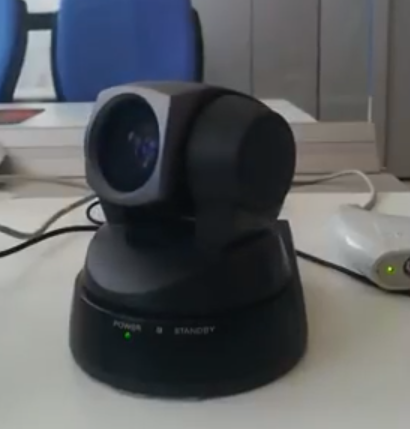
\includegraphics[width=0.88\linewidth, height=6.0cm]{figures/sonyevi.png}
		\caption{Cámara Sony Evi d1oop}
		\label{fig.sonyevi}
		\end{center}
\end{figure}
\begin{itemize}
	\item[--] 440,000 pixeles que permiten tomas en alta resolución.
	\item[--] Además de la acción de Pan y Tilt de alta velocidad, la mejora del mecanismo de reducción de ruido para vídeo en color. 
	\item[--] Posibilidad de operación desde computador a través de VISCA.
	\item[--] Buffer de mensajes que permite memorizar hasta 6 combinaciones de la posición y el estado de la cámara. 
	\item[--] Control remoto multifunción. 
	\item[--] Compatibilidad de comandos con modelos anteriores.
\end{itemize}
\end{multicols}

\begin{multicols}{2}
Dado que el hardware captura vídeo analógico, en combinación con la cámara se ha usado una capturadora de vídeo, que es un periférico de entrada cuya función es recibir señales de audio/video procedentes de dispositivos analógicos y convertirlas en señales digitales que puedan ser almacenadas o manipuladas por medio de software.
\begin{figure}[H]
  \begin{center}
    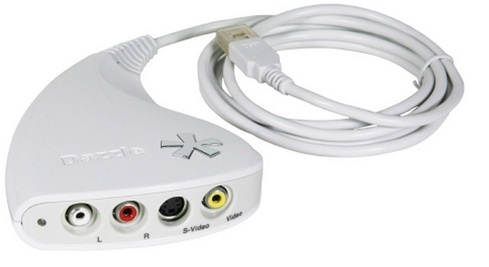
\includegraphics[width=0.55\linewidth, height=4.0cm]{figures/capturadora.jpg}
		\caption{Digitalizador Dazzle DVD Recorder}
		\label{fig.digitalizadora}
		\end{center}
\end{figure}
\end{multicols}
La capturadora utilizada es Dazzle DVD Recorder HD de la marca Pinnacle (\textbf{Figura 4.2}), y con conexión USB 2.0 con el ordenador. En cuanto a las capacidades del hardware en conjunto, nos interesan:

El valor de \textit{Pan} puede estar entre -164º y 164º y su velocidad puede tomar valores en un rango donde 1 es el mínimo y 24 es el máximo.

De forma análoga, el valor de \textit{Tilt} puede oscilar entre -30º y  30º, con velocidades en una escala de 1 a 20.

Por lo demás, la cámara utilizará \textit{drivers} para el acceso a la imagen y a los actuadores y para la comunicación con el nodo académico.

\subsection{Driver ROS usb\_cam}
El \textit{driver} usb\_cam interactúa con cámaras USB estándar (por ejemplo, SonyEvi d100p o Logitech Quickcam) utilizando libusb\_cam\footnote{\url{https://github.com/libusb/libusb/wiki}}, una biblioteca multiplataforma para acceso genérico a dispositivos USB, y publica imágenes bajo el formato de mensajes \textit{sensor\_msgs::Image}\footnote{\url{http://docs.ros.org/api/sensor\_msgs/html/msg/Image.html}} 
 de ROS. Además, utiliza la biblioteca \textit{image\_transport}\footnote{\url{http://wiki.ros.org/image\_transport}} para permitir el transporte de imágenes comprimidas.

A través de él obtendremos las imágenes que proporciona la cámara. Dado que es un driver de ROS, emplea la herramienta \textit{roslaunch}\footnote{\url{http://wiki.ros.org/roslaunch}}, que permite lanzar fácilmente múltiples nodos ROS de manera local o remota. Para ello, necesita un fichero de configuración XML como el siguiente: 

\begin{figure}[H]
  \begin{center}
    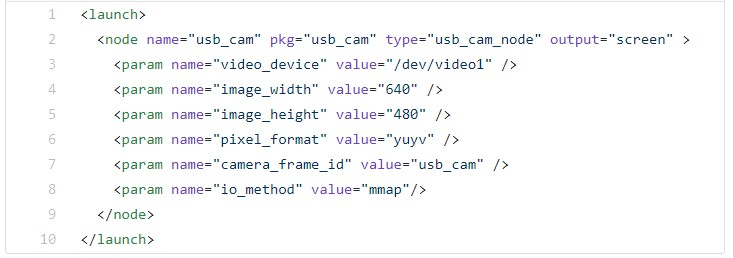
\includegraphics[width=0.99\linewidth]{figures/usbcamconf.jpg}
		\caption{Fichero de configuración de usb\_cam}
		\label{fig.usbcamconf}
		\end{center}
\end{figure}

En él deben especificarse los parámetros del nodo o nodos a establecer, así como los dispositivos sobre los cuales se lanza el nodo, en nuestro caso, la cámara (\textit{/dev/video1}).

\subsection{Driver Teleoperador Evicam}
El \textit{driver} Evicam ha sido desarrollado e incluido en la plataforma JdeRobot para poder teleoperar cámaras vía software a través de una conexión USB. En concreto, utiliza una interfaz ICE para poder controlarla a través de comandos de movimiento. 
El código fuente puede encontrarse en: 

\url{https://github.com/JdeRobot/JdeRobot/tree/master/src/drivers/evicam_driver}

Este driver debe lanzarse también con un fichero de configuración que indique el par \textit{IP:puerto} en el que la cámara espera órdenes y el dispositivo. Un ejemplo se muestra en la \textbf{Figura 4.4}:

\begin{figure}[H]
  \begin{center}
    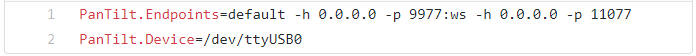
\includegraphics[width=0.99\linewidth]{figures/evicamconf.png}
		\caption{Fichero de configuración de evicam\_driver}
		\label{fig.evicamconf}
		\end{center}
\end{figure}

\section{Componente Académico}
El componente académico de esta práctica resuelve varias funcionalidades auxiliares que sirven de gran ayuda para poder abordarla:

\begin{enumerate}[label=\alph*)]
	\item Ofrece una interfaz gráfica al usuario que le ayuda a depurar su código; 
	\item Ofrece acceso a la cámara y a sus actuadores en forma de métodos simples (oculta el \textit{middleware} de comunicaciones con el hardware);  
	\item Incluye código auxiliar que no es el foco del algoritmo y que ayuda a programar la solución.
\end{enumerate}

El componente deja todo preparado para que el estudiante sólo tenga que incluir su código retocando el método \textit{execute} en el fichero \textit{MyAlgorithm.py}, e ir realizando las pruebas pertinentes.

El componente ofrece un API de cámara y actuadores al programador con el cuál acceder a la funcionalidad que necesita:

\begin{itemize}
	\item \textit{self.camera.getImage()}: devuelve la imagen capturada por la cámara activa (local o cámara usb).
	\item \textit{self.camera.setColorImage(img)}: método que recibe una imagen y la muestra en el espacio dedicado del interfaz para imágenes capturadas.
	\item \textit{self.camera.setThresholdImage(img)}: método que recibe una imagen tratada y la muestra en el espacio reservado en el GUI para imágenes filtradas, umbral o en blanco y negro.
	\item \textit{self.motors.getLimits()}: método a través del cual se pueden obtener los límites de Pan y Tilt (en grados).
	\item \textit{self.motors.setPTMotorsData(pan, tilt, panSpeed, tiltSpeed)}: método para enviar comandos de \textit{Pan} y \textit{Tilt} a la cámara. Necesita los valores respectivos en grados y la velocidad horizontal y vertical para alcanzar la posición fijada.
\end{itemize}

El nodo académico requiere un fichero de configuración que indique los \textit{endpoints} que utilizan la cámara y los motores PT. Este archivo tiene extensión \textit{.yml}, lo cual implica que debe seguir el formato de serialización de datos YAML, el cual produce datos fáciles de leer por humanos y máquinas para todos los lenguajes de programación. Tiene el siguiente aspecto:

\begin{figure}[H]
  \begin{center}
    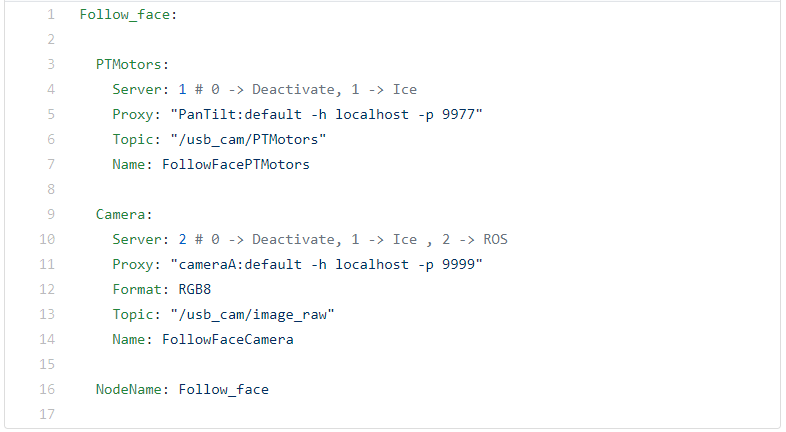
\includegraphics[width=0.99\linewidth]{figures/ymlfollowface.png}
		\caption{Fichero de configuración YAML de FollowFace}
		\label{fig.followfaceconf}
		\end{center}
\end{figure}

Se puede ver claramente que las interfaces empleadas por cámara y motores son distintas, siendo en el primer caso ROS y en el segundo ICE, como ya se explicó. Se observa también que puede incluir información adicional, como el formato de imagen.

En cuanto a la capacidad de cómputo para realizar todas las tareas simultáneamente, el componente emplea dos hilos de ejecución para agilizar la respuesta de los distintos módulos:
\begin{itemize}
	\renewcommand{\labelitemi}{$\to$}
	\item Hilo de algoritmo: se encarga del refresco de la ejecución del algoritmo, ya que este se ejecuta de modo cíclico. El tiempo de refresco de este hilo es muy importante, dado que su velocidad permitirá reaccionar ante situaciones imprevistas, y adaptar el movimiento de la cámara a la velocidad de movimiento de las personas, para poder seguir su cara. Es por eso que el tiempo de refresco es de 80 ms.
	\item Hilo de la interfaz gráfica de usuario (GUI): Este hilo es el encargado de actualizar la interfaz gráfica. También consta de los manejadores de eventos del GUI. El intervalo de actualización de la interfaz debe ser pequeño, ya que se tiene que mostrar las imágenes captadas por la cámara en forma de elemento vídeo, así como las imágenes segmentados en tiempo real. Por ello, se ha fijado el tiempo de refresco a 50 ms.
	
	Por último, el nodo académico incluye dos ficheros de descripción XML, que servirán de entrenamiento para los clasificadores que necesitaremos en la segmentación, explicados con mayor detalle en el apartado \textbf{4.4}. 
\end{itemize}

\subsection{Interfaz gráfica}
La interfaz gráfica de usuario (GUI) de la práctica sirve para representar información importante para desarrollar correctamente el algoritmo que lleve a la solución, además de para proporcionar funcionalidad básica para iniciar o para el algoritmo o para teleoperar la cámara. Se ha programado en Python con PyQt5, y es la mostrada en la \textbf{Figura 4.6}.

\begin{figure}[H]
  \begin{center}
    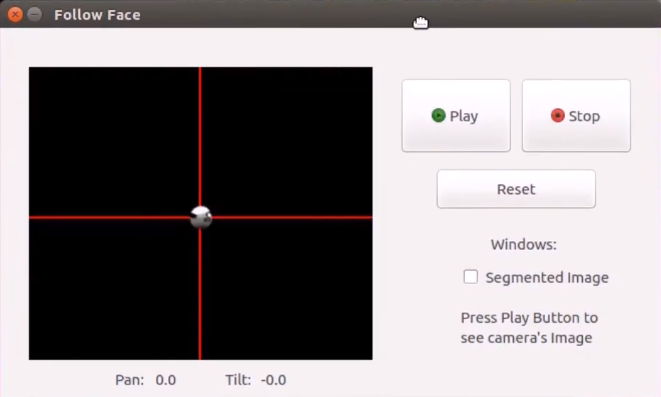
\includegraphics[width=0.99\linewidth]{figures/guifollowface.png}
		\caption{Interfaz Gráfica de Follow Face}
		\label{fig.guifollowface}
		\end{center}
\end{figure}

Se puede ver en ella, a la izquierda, el teleoperador para comprobar que el movimiento de la cámara este operativo. Se trata de un dial bidimensional que controla las componentes \textit{Pan} y \textit{Tilt} del robot. Únicamente será necesario mover el \textit{joystick} central en sentido vertical, para controlar el ángulo de \textit{Pan} y en sentido horizontal para fijar el \textit{Tilt}. Cuánto más se acerque el \textit{joystick} a los límites del teleoperador, más acentuado será el valor de la componente hacia la que se esté movimiento el mismo, ya sea éste un valor negativo si se mueve hacia abajo o hacia la izquierda, y positivo en caso de que se mueva hacia arriba o a la derecha. A su derecha, se han colocado varios botones cuya funcionalidad es la de iniciar el algoritmo, pararlo o resetearlo. Recordemos que la cámara dispone de un \textit{buffer} de mensajes, de manera que pulsar el botón Stop se traducirá en pausar el algoritmo, pero la cámara puede continuar en movimiento si había encolado mensajes, hasta que vacíe dicho \textit{buffer}. Inmediatamente debajo tenemos un \textit{check} que muestra la herramienta de imagen (\textbf{Figura 4.7}), en la cual se pueden ver las imágenes que provee la cámara (a la izquierda) y la imagen segmentada (a la derecha, en caso de haberla establecido):

\begin{figure}[H]
  \begin{center}
    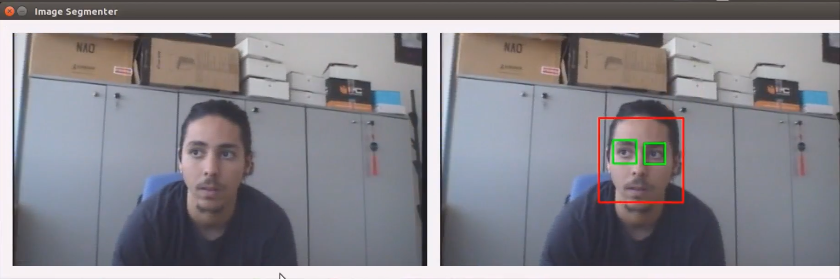
\includegraphics[width=0.99\linewidth]{figures/imagetool.png}
		\caption{Herramienta de imagen}
		\label{fig.imagetool}
		\end{center}
\end{figure}

\subsection{Código auxiliar: Clase CameraSegment}
Dentro del componente académico existe la clase \textit{CameraSegment}. Esta clase se ha creado por controlar y establecer la visualización de las imágenes que tienen que ver con la práctica, sustituyéndolas por imágenes negras si son nulas o estableciendo el vídeo capturado por la cámara y el vídeo segmentado creado y seleccionado por el programador.

El objeto \textit{self.camera} del cual dispone el algoritmo se construye a partir de ésta clase, por lo cual incluye algunos métodos propios además que los esperados por la cámara. Hablamos de las funciones que permiten mostrar las imágenes en el interfaz, descritas en \textbf{4.3}. Por tanto, actúa de nexo entre la herramienta de segmentación (\textit{segment widget}) y el algoritmo, proporcionando un API fácil de utilizar.

Por último, esta clase actúa de intermediario entre la cámara y el interfaz, conectando ambos componentes. Esto es necesario dado que las imágenes capturadas por la cámara y las que espera el interfaz no son completamente compatibles: para poder ser visualizadas, las imágenes deben redimensionarse para encajar en la aplicación gráfica.

\section{Solución de referencia}
Dado que el objetivo de la práctica es conseguir que el robot siga caras, la solución ha de contener un algoritmo de segmentación de imagen y otro de pilotaje, ambos respondiendo a un control reactivo. 
En esta sección, abordaremos brevemente los fundamentos de segmentación y detección de caras y el control gradual de hardware. Con ello construiremos una solución que se establecerá como solución de referencia en la plataforma, pero que sólo es uno de los muchos posibles métodos con el cual alcanzar el fin. El código quedara recogido en el fichero \textit{MyAlgorithm.py} que, como ya sabemos, es de naturaleza iterativa, de manera que en cada iteración se percibe, se actúa en consecuencia y se controla. Se habrá de escribir el método \textit{execute}, el cual debe contener la lógica que se ejecuta de manera cíclica en el \textit{thread} de algoritmo y computación.

\subsection{Fundamentos de la Detección de caras}
Las cámaras que incorporan los robots son una de las principales fuentes de información con las que cuentan, pero toda esta información es inútil sin la lógica que sea capaz de extraer la información relevante de la imagen. Incluso, algoritmos incapaces de diferenciar lo necesario de lo inane sólo conseguirán sobrecargar a la máquina de información inoperante, reduciendo su rendimiento e incluso llegando a producir comportamientos indeseados. Es por eso que es fundamental un buen algoritmo de detección de caras en la imagen, sobre todo cuando se trata de controlar un robot real con los datos extraídos y procesados. 

La detección de rostros se puede considerar como un caso específico de detección de “clases de objetos”. En la detección de clase de objeto, la tarea es encontrar las ubicaciones y tamaños de todos los objetos en una imagen que pertenecen a una clase determinada. Algunos ejemplos muy comunes en casos reales son torsos superiores, peatones y automóviles. De la misma forma, debemos ser capaces de encontrar caras en una imagen digital, sea cual sea su tamaño o ubicación en ella. Existen muchos algoritmos de detección de rostros para ubicar a una persona en una escena, algunos más fáciles y otros más complejos:

Cuando la imagen consta de un fondo monocolor simple o un fondo estático predefinido (conocido), es muy fácil detectar caras, dado que eliminar dicho fondo siempre tendrá como resultado los límites de la cara. Sin embargo, sabemos que en nuestro caso el robot debe comportarse correctamente en cualquier escenario, de manera que no es una solución válida.

Otra manera pasa por utilizar el color de piel típico para encontrar segmentos faciales, si se dispone de imágenes en color. La desventaja en este caso es que no funcionará con todo tipo de colores de piel, y que su robustez es mínima ante condiciones de iluminación variables. 

Existen otras técnicas basadas en la suposición de que las caras siempre estarán en movimiento en una secuencia de vídeo, de manera que calcular el área de movimiento se puede proporcionar una estimación. Todas ellas son poco robustas, pero juntas (y añadiendo algunos otros extras) se puede componer una buena aproximación a la solución. 

Sin embargo, y aunque resulte sorprendente, la forma de abordar esta tarea con mayor éxito es utilizar imágenes en escala de grises, con lo cual reducimos el coste computacional (requisito fundamental en aplicaciones en tiempo real). A su vez, hay varios métodos que las emplean, como son la detección basada en modelo, en emparejamiento de bordes por orientación, usando la distancia de Hausdorff\footnote{\url{https://en.wikipedia.org/wiki/Hausdorff_distance}},etc. Pero el más utilizado es mediante el uso de "clasificadores en cascada" encapsulado dentro de las técnicas de aprendizaje máquina que, utilizando características simples de Haar, puede producir resultados impresionantes.

El aprendizaje máquina o \textit{machine learning}, es una técnica empleada en el campo de las ciencias de computación y de estadística que aporta a las máquinas la capacidad de aprender en base a la observación de sucesos y decidir a partir de ellos. Así, un clasificador actúa de tal manera que “memoriza” la categoría asignada a un conjunto de sucesos conocidos (\textit{training group}), y a parir de ellos es capaz de realizar una inferencia o razonamiento inductivo, extrayendo características de los ejemplos del conjunto de entrenamiento y comparándolas con características de la misma naturaleza de nuevos ejemplos que entren al sistema. Únicamente habrá que dotar a la máquina de principios bien definidos que eviten que extraiga conclusiones inútiles. Con todo ello, una tarea extremadamente difícil de programar como podría ser reconocer todas y cada una de las caras existentes, se hace posible a través de este mecanismo capaz de clasificarlas sin haberlas visto antes.

Hay muchas motivaciones para usar características en la comparación en lugar de hacerlo con los píxeles directamente. La razón más común es que las características pueden codificar conocimiento del dominio ad-hoc, lo cual es difícil usando una cantidad finita de datos de entrenamiento. Para este sistema también hay una segunda motivación crítica para emplear características: el sistema basado en características funciona mucho más rápido que un sistema basado en píxeles. Estas características son las que se muestran en la siguiente imagen (\textbf{Figura 4.8}):

\begin{figure}[H]
  \begin{center}
    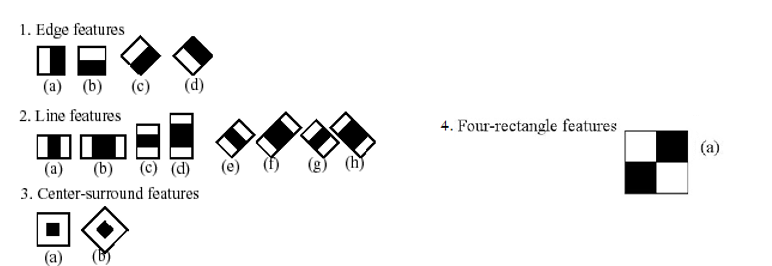
\includegraphics[width=0.99\linewidth]{figures/features.png}
		\caption{Características de comparación}
		\label{fig.features}
		\end{center}
\end{figure}

Cada “ventana” de las de la imagen se coloca en la imagen a segmentar para calcular una sola característica. Esta característica es un valor único que se obtiene al restar la suma de píxeles debajo de la parte blanca de la ventana de la suma de los píxeles debajo de la parte negra de la ventana. Así, todos los tamaños posibles de cada ventana se colocan en todas las ubicaciones posibles de cada imagen para calcular muchas características. 

\begin{figure}[H]
  \begin{center}
    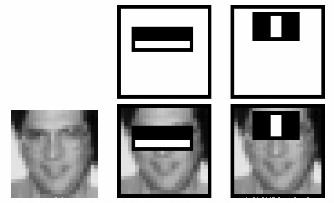
\includegraphics[width=0.69\linewidth]{figures/extraction.jpg}
		\caption{Extracción de características}
		\label{fig.extraction}
		\end{center}
\end{figure}

Por ejemplo, en la \textbf{Figura 4.9}, estamos extrayendo dos características. La primera se centra en la propiedad de que la región de los ojos a menudo es más oscura que el área de la nariz y las mejillas. La segunda característica se basa en la propiedad de que los ojos son más oscuros que el puente de la nariz.

Pero entre todas estas características calculadas, la mayoría de ellas son irrelevantes. Por ejemplo, cuando se usa en la mejilla, las ventanas se vuelven irrelevantes porque ninguna de estas áreas es más oscura o más clara que otras regiones en las mejillas, todos los sectores en ella son iguales. Por lo tanto, se debe descartar de inmediato las características irrelevantes y conservar únicamente aquellas importantes con una técnica llamada \textit{Adaboost} que selecciona solo aquellas características conocidas para mejorar la precisión de clasificación (cara / no cara) del clasificador. Finalmente, el algoritmo considera el hecho de que, en general, la mayor parte de la región en una imagen es una región sin cara. Teniendo en cuenta esto, es mejor idea tener un método simple para verificar si una ventana es una región sin rostro, y si no lo es, desecharla de inmediato y no volverla a procesar. Así el clasificador es capaz de enfocarse principalmente en el área donde exista una cara. Es por eso por lo que reciben el nombre de clasificadores en cascada (\textbf{Figura 4.10}), dado que se usan en primera instancia clasificadores simples para descartar esas áreas y luego clasificadores más complejos para eliminar falsos positivos.

\begin{figure}[H]
  \begin{center}
    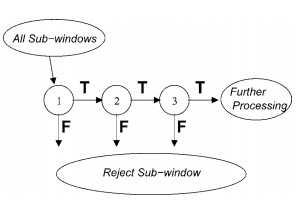
\includegraphics[width=0.50\linewidth, height=4cm]{figures/cascade.jpg}
		\caption{Clasificadores en cascada}
		\label{fig.cascade}
		\end{center}
\end{figure}

Esto permite reducir en gran medida la computación. Con ello, los sucesivos clasificadores son entrenados con las muestras que pasan las etapas anteriores. Un clasificador en cascada bien entrenado (incluyendo positivos y negativos), será capaz de identificar en una imagen dada si existen caras en ella, sea cual sea su origen, color, tamaño y posición con la parametrización adecuada.

\subsubsection{Clasificadores Máquina}
Como ya se ha visto, la manera escogida para abordar la tarea de detección pasa por utilizar un clasificador en cascada. 
Estudiando la librería OpenCV para Python, hemos encontrado la manera de crear entrenadores y detectores, los cuales se pueden entrenar de la forma que se desee. Además la librería incluye sistemas pre-entrenados para detectar facciones concretas de la cara como ojos, sonrisa, cejas e incluso la cara en sí.

Estos sistemas de entrenamiento se encuentran en ficheros XML provistos por la librería, dos de los cuales se han incluido en el nodo académico de esta práctica para poder abordarla siguiendo este método propuesto por  Paul Viola y Michael Jones en su \textit{paper}, \textit{"Rapid Object Detection using a Boosted Cascade of Simple Features"} en 2001. Estos ficheros son:

\textit{haarcascade\_frontalface\_default.xml} $\rightarrow$ entrenamiento para detectar caras en posición frontal.

\textit{haarcascade\_eye.xml} $\rightarrow$entrenamiento para clasificador de ojos.

Con ellos es suficiente para realizar un proceso de detección y segmentación genérico y en condiciones normales. El alumno tiene la posibilidad de entrenar todos los clasificadores que quiera para su programa, simplemente incluyendo los ficheros \textit{.xml} necesarios en el directorio de trabajo. Una vez obtenidos, simplemente se invocará la función:

\begin{figure}[H]
  \begin{center}
    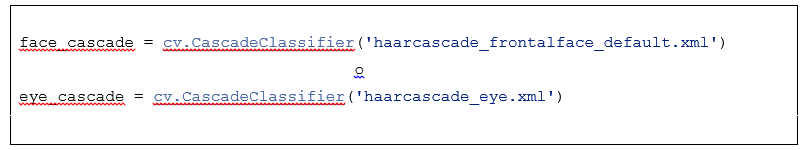
\includegraphics[width=0.99\linewidth]{figures/classifiercode.png}
		\label{fig.classifiercode}
		\end{center}
\end{figure}
Para obtener un objeto Python con el clasificador deseado.

\subsubsection{Eliminación de falsos positivos}
Usar clasificadores en cascada es la mejor manera de reducir la tasa de falsos positivos en la detección. Sin embargo, bajo condiciones cambiantes de luminosidad o entornos con mucho contenido se tienen resultados etiquetados como positivos en casos que claramente no lo son (\textbf{Figura 4.11}):

\begin{figure}[H]
  \begin{center}
    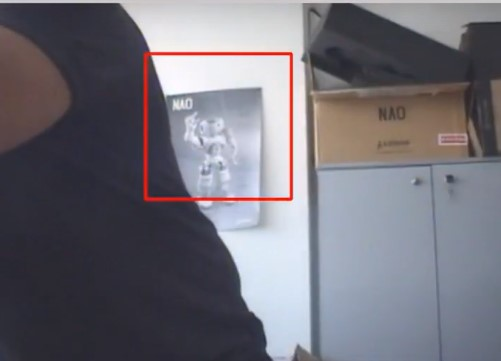
\includegraphics[width=0.70\linewidth]{figures/falsopositivo.jpg}
		\caption{Falso positivo}
		\label{fig.falsopositivo}
		\end{center}
\end{figure}

Proporcionar al sistema un entrenamiento más meticuloso sería la opción ideal para reducir aún más la tasa de error. Sin embargo, las prácticas en este entorno buscan que el alumno se enfrente únicamente a la lógica de control y obtención de datos de los robots, de manera que este problema debe abordarse con código de filtrado de los resultados.

Con ello, tras obtener la posición de todas las caras de la imagen con el método \textit{detectMultiScale} del objeto clasificador de OpenCV (en nuestro caso, \textit{face\_cascade}), aplicamos un filtrado del output que elimine positivos de tamaño inferior a un umbral mínimo, o superior a un umbral máximo para mejorar los resultados. Además, incluimos un clasificador para la detección de ojos que resultará más restrictivo a la hora de hacer una detección final. Finalmente, se utiliza la función \textit{rectangle} del paquete con las coordenadas de la cara para hacer visual la detección. Una vez aplicado el filtro, el resultado cambia (\textbf{Figura 4.12}):

\begin{figure}[H]
  \begin{center}
    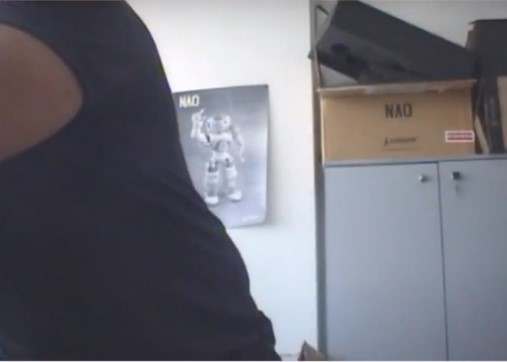
\includegraphics[width=0.70\linewidth]{figures/falsopositivosolved.jpg}
		\caption{Falso positivo solucionado}
		\label{fig.falsopositivosolved}
		\end{center}
\end{figure}

\subsection{Control PT de la cámara}
Dentro del grupo de las cámaras móviles, uno de los grandes subgrupos es el de las cámaras PTZ. Estas siglas indican el control que se puede ejercer sobre la máquina, siendo que se puede modificar el valor que toma en \textit{Pan} (P), el que toma en \textit{Tilt} (T) y el que toma de \textit{zoom} (Z). Nuestra cámara no dispone de \textit{zoom}, se podría decir que consta de un control PT.

Ahora bien, tratándose de control en tiempo real, ¿puede tomar cada componente cualquier valor dentro de los límites del hardware? Evidentemente no. En estos casos debemos contar con el tiempo físico que tarda la cámara en ejecutar el movimiento solicitado. También debe tenerse en cuenta el \textit{buffer} asociado, que encola mensajes hasta que puedan ser atendidos. Si se envía la misma orden dos veces antes de que el hardware sea capaz de terminar la primera (algo muy común), el resultado se traducirá en un “temblor” u oscilación de la cámara entorno a esos valores.

Es por eso que a lo largo del apartado hemos hablado de control gradual. En aplicaciones de este tipo, se hace necesario que el movimiento del cuello mecánico sea a la vez fluido y suave, sin ejecutar movimientos demasiado bruscos, y sin oscilaciones que repercutan en la calidad de la imagen captada, para que el algoritmo pueda seguir funcionando de manera óptima durante los movimientos.
Por ello, hemos decidido implementar un control que trabaje en incrementos o sustracciones pequeñas en grados de los valores \textit{Pan} y \textit{Tilt}. Con ello conseguimos también aprovechar la máxima velocidad de movimiento que ofrece el hardware, sin balanceos, obteniendo un movimiento adecuado en combinación con el tiempo de refresco del hilo de ejecución de algoritmo. En cada iteración, habrá que calcular el centro de la cara detectada y trabajar para que dicho centro coincida con el centro de la imagen captada. En caso de no ser así, se obtendrá el error de posición y se modificarán los valores de control de la cámara de la forma conveniente. En caso de coincidencia, se detendrán los motores y se hará que la cámara permanezca en espera al próximo movimiento.

\subsection{Gestión de la ``No Detección''}
Llegados a este punto se ha llevado a cabo la tarea principal que planteaba esta práctica. Sin embargo, la funcionalidad no es del todo completa. Hemos programado el comportamiento en caso de detección, la eliminación de falsos positivos, la lógica de control y la segmentación pero, ¿qué hace el programa propuesto en caso de no detectar caras en la imagen?

Existen varios caminos posibles:

\begin{itemize}
	\item[--] El primero sería simplemente no hacer nada. El hardware permanece en espera a que una persona entre en escena. Se establece un módulo condicional en el código que detiene los motores en la posición actual si no detecta rostros. No obstante, se puede evolucionar la solución a través de otras vías.
	\item[--] Una segunda opción sería volver a la posición de reposo, de la cual parte la cámara en el primer instante de ejecución. Esto se reflejaría en tener un mayor rango de movimiento cuando una persona vuelva a aparecer en la imagen. Si el clasificador deja de detectar caras cerca del límite físico del cuello mecánico, esta solución lo haría volver al centro, aumentando el margen de movimiento para la próxima detección.
	\item[--] Por último, la solución por la que nos hemos decantado ha sido por iniciar un proceso de búsqueda de rostros dentro del “campo de visión” de la cámara. 
\end{itemize}

Cuando en la imagen no se encuentran secciones que casen con una cara, la cámara esperará 5 segundos como margen para seguir comprobando en las siguientes iteraciones si realmente no hay caras visibles, o si por el contrario se trataba de un error de clasificación. Pasados estos 5 segundos, la cámara comienza un movimiento horizontal (a lo largo del eje X) hacia la derecha, dado que este eje es en el que más probabilidad existe de encontrar una cara, no sólo por las características de las personas (no podemos desplazarnos en vertical, volar), sino también porque es el eje con mayor recorrido del hardware: 328º frente a 60º. Mientras se desplaza sigue ejecutando el algoritmo de detección, de manera que en caso de obtener un positivo, se continúa con la ejecución normal de seguimiento y, en caso contrario, se efectúa el movimiento hasta que se llegue al extremo. Una vez en el extremo, efectúa el mismo movimiento hacia el otro lado. La cámara permanecerá en movimiento en todo momento hasta la detección de una nueva cara.

\section{Experimentación}
En este apartado demostraremos la funcionalidad descrita en los apartados anteriores a través de experimentos realizados para poner a prueba tanto la infraestructura de la práctica, como el nodo y la solución.

\subsection{Ejecución típica}
Se ha preparado un documento de texto (\textit{README.md}) que sirve de guía para que alumno no encuentre dificultades durante la ejecución y el testeo, que incluye también información del API de utilización. 

La forma de ejecutar la práctica es la siguiente:

\begin{enumerate}
	\item Empleamos un primer terminal para inicial el driver de ROS \textit{usb\_cam} (previamente habrá que asegurarse de haber instalado el paquete \textit{ros-kinetic-usb-cam packet}):
	\begin{figure}[H]
		\begin{center}
			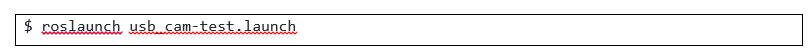
\includegraphics[width=0.95\linewidth]{figures/ffcomando1.png}
			\label{fig.ffcomando1}
		\end{center}
	\end{figure}
	\item Utilizamos un segundo terminal para iniciar el driver \textit{evicam\_driver}:
	\begin{figure}[H]
		\begin{center}
			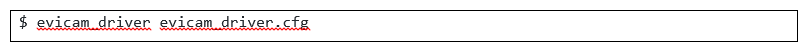
\includegraphics[width=0.95\linewidth]{figures/ffcomando2.png}
			\label{fig.ffcomando2}
		\end{center}
	\end{figure}
	\item 3.	Por último, se lanza en otro terminal el componente \textit{follow\_face}:
	\begin{figure}[H]
		\begin{center}
			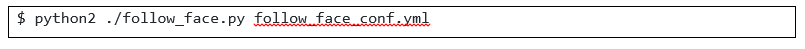
\includegraphics[width=0.95\linewidth]{figures/ffcomando3.png}
			\label{fig.ffcomando3}
		\end{center}
	\end{figure}
\end{enumerate}

Una vez implementada la solución, el \textit{output} debe ser similar al siguiente (\textbf{Figura 4.13}):

\begin{figure}[H]
  \begin{center}
    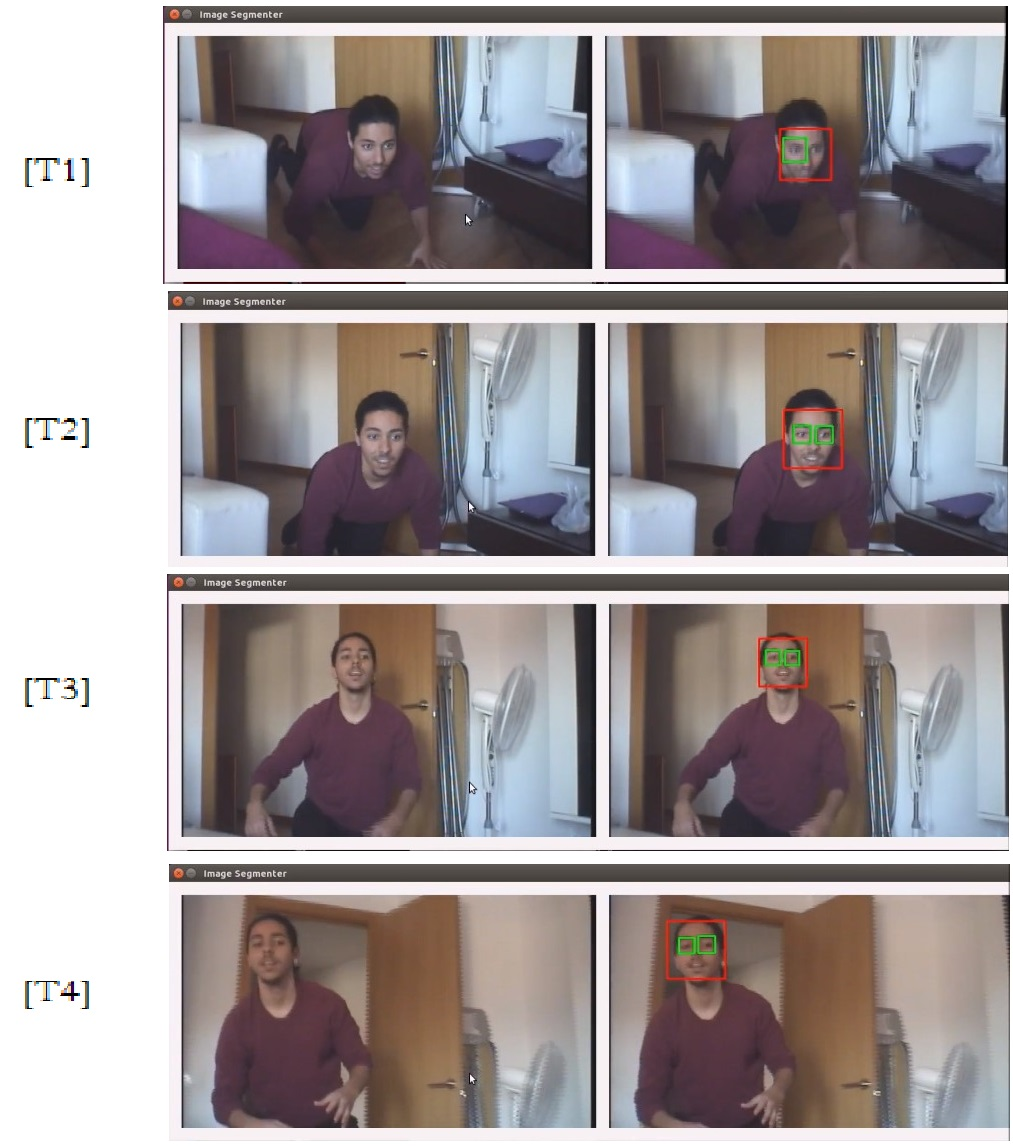
\includegraphics[width=0.98\linewidth]{figures/ffoutput.jpg}
		\caption{Output Follow Face}
		\label{fig.ffoutput}
		\end{center}
\end{figure}

Ejemplos de la ejecución pueden encontrarse en:
 
\url{https://www.youtube.com/watch?v=pdSPnftumf8}, y
 
\url{https://www.youtube.com/watch?v=YZEMIXkXwM0}

\subsection{Comportamiento ante casos extremos}
Como hemos comentado, hemos tratado de poner el algoritmo a prueba para comprobar su validez:

Una primera situación que debimos probar fue la ejecución con movimiento rápido. La persona al frente de la cámara se movió de manera brusca, cambiando de dirección y con subidas y bajadas periódicas. Gracias al movimiento gradual implementado, el algoritmo es capaz de seguir en todo momento el movimiento, salvo en aquellos casos en los que el sujeto se sale bruscamente del plano. 

Por otro lado, probamos la ejecución en situaciones de contraluz. En este caso, el comportamiento empeoraba, ya que la imagen captada, al convertirse a escala de grises, no mostraba apenas diferencia de niveles en pixeles que conforman secciones de la cara que normalmente si presentan dicha diferencia. Esto se debe a las bases de la detección con clasificadores en cascada. Se podría tratar de solucionar incorporando técnicas de detección de color de piel, entre otras.

Por último, en situaciones con muchos candidatos a caras (posters, muñecos y elementos con formas abstractas), el algoritmo se equivocaba el 5\% de las veces, siendo que en el resto de casos escogía el candidato correcto para seguir.

\section{Follow\_Face a través de Jupyter}
En el apartado \textbf{3.6} se introdujo la herramienta Jupyter Notebook,  que permite al usuario crear y compartir documentos que contengan multitud de elementos y widgets programables a través de distintos lenguajes. Hemos aprovechado la funcionalidad de la aplicación para dar un paso más hacia una práctica multiplataforma.
Durante la investigación sobre este proyecto, comprendimos la potencia y prestaciones que ofrece Jupyter, de manera que decidimos adaptar un nodo y una solución a través de esta herramienta. Con él, y utilizando herramientas en desarrollo de JdeRobot y GzWeb\footnote{\url{http://gazebosim.org/gzweb.html}}, más adelante se adaptará un servidor que contenga todo lo necesario para lanzar las prácticas, y que se apoye en interfaces locales como la simulación para alcanzar la independencia de plataforma.

Antes de comenzar, debe instalarse el código del proyecto, proceso del que se detallen las instrucciones en la página oficial del proyecto\footnote{\url{http://jupyter.org/install}}.

Hemos preparado un \textit{Notebook} de Jupyter al que hemos llamado \textit{follow\_face.ipynb}, que junto con algunos cambios en la estructura del nodo académico proporcionan el soporte necesario para tener la misma práctica disponible a través de esta aplicación. En concreto, el nodo programado en el fichero \textit{follow\_face.py} de la práctica original ha sido recodificado para tener estructura de clase Python: la clase \textit{FollowFace}, para poder ser instanciada desde el código del cuadernillo, que detallaremos un poco más adelante. Los cambios más significativos se producen al habernos desecho de la interfaz gráfica, dado que será ahora la propia aplicación la que actúe de interfaz de usuario. Eliminados los componentes gráficos y los widgets que mostraban las imágenes en él, se ha hecho crear una nueva clase (la clase \textit{Printer}, \textbf{Figura 4.14}) que nos permita visualizar las imágenes que el alumno establece a través de métodos disponibles en la clase nodo (\textit{FollowFace}) en la interfaz de Jupyter. Para ello, utilizamos los métodos disponibles en la librería \textit{matplotlib} y su módulo \textit{pyplot},  una colección de funciones cuyo estilo es como un comando que hacen que \textit{matplotlib} funcione como MATLAB en cuanto a representaciones, lo cual simplifica mucho la visualización en la herramienta. 

\begin{figure}[H]
  \begin{center}
    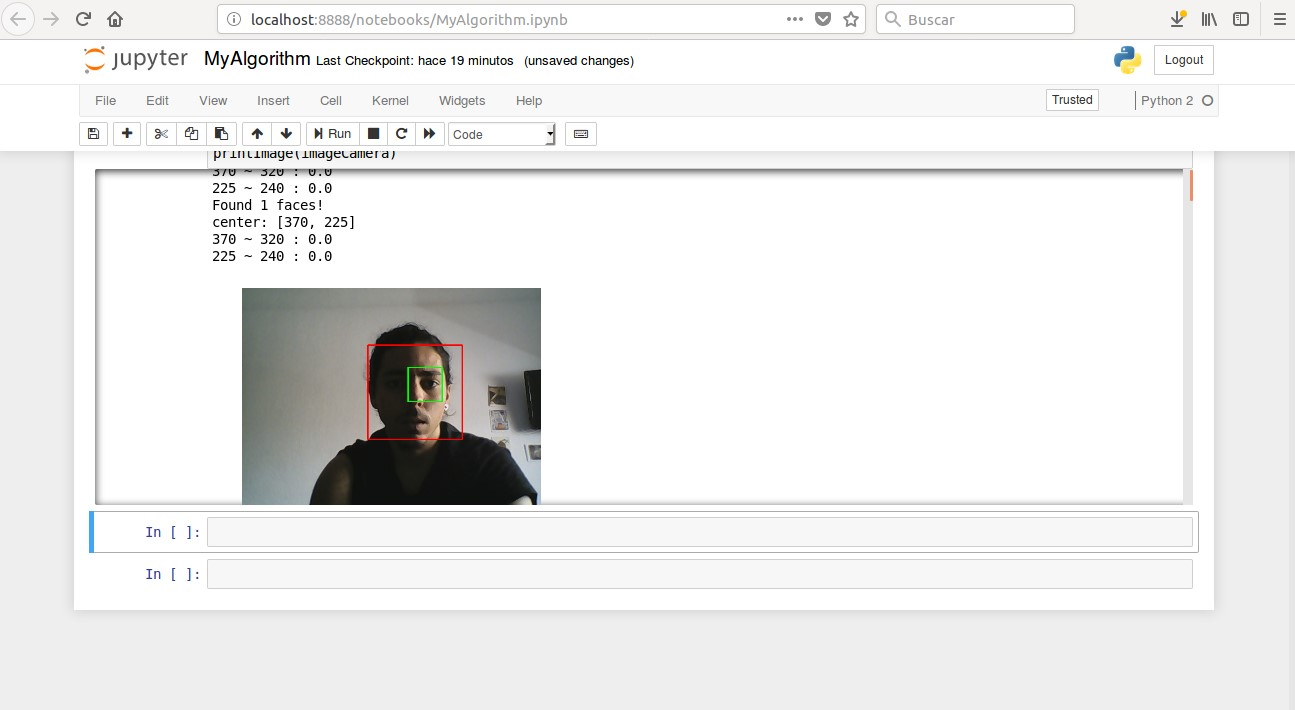
\includegraphics[width=0.98\linewidth]{figures/printer.jpg}
		\caption{Printer}
		\label{fig.printer}
		\end{center}
\end{figure}

Con todo ello, únicamente queda asociar el código del cuadernillo con el del nodo, lo cual conseguimos a través de la librería \textit{types} de Python. Esta librería proporciona acceso a los nombres de algunos tipos de objetos que son utilizados por el intérprete estándar de Python, de manera que podemos modificar el comportamiento normal de los mismos. Utilizaremos la función \textit{MethodType} para hacer corresponder la función que el estudiante retoca desde la aplicación de Jupyter con el método que realiza el cómputo en el hilo de algoritmo del nodo académico modificado. Por último, hemos de recordar que necesitamos de la intervención de dos \textit{drivers} para controlar la cámara de la que disponemos, de manera que la adaptación del nodo incorpora el lanzamiento de dos subprocesos, uno para cada \textit{driver}, a través de la librería \textit{subprocess}, que permite generar nuevos procesos y conectarse a sus tuberías de entrada / salida / error, además de obtener sus códigos de retorno. Con esto, y unas pequeñas incorporaciones al nodo para poder parar o ejecutar el algoritmo desde Jupyter, completamos la práctica a través de la aplicación. 

Entrando ya en el cuadernillo o \textit{Notebook} generado (\textbf{Figura 4.15}), éste no sólo incorpora celdillas de código ejecutable embebidas, sino que también incluye imágenes representativas y texto descriptivo para orientar al alumno en todo momento (durante la ejecución, aportando información adicional para abordar la práctica y explicando el API de utilización con los nuevos métodos de visualización y actualización del código. 

Así, el alumno puede abordar la práctica de manera totalmente guiada, y ejecutar los distintos pasos que va abordando para observar su salida, con herramientas disponibles para depurar errores o matizar su solución.

\begin{figure}[H]
  \begin{center}
    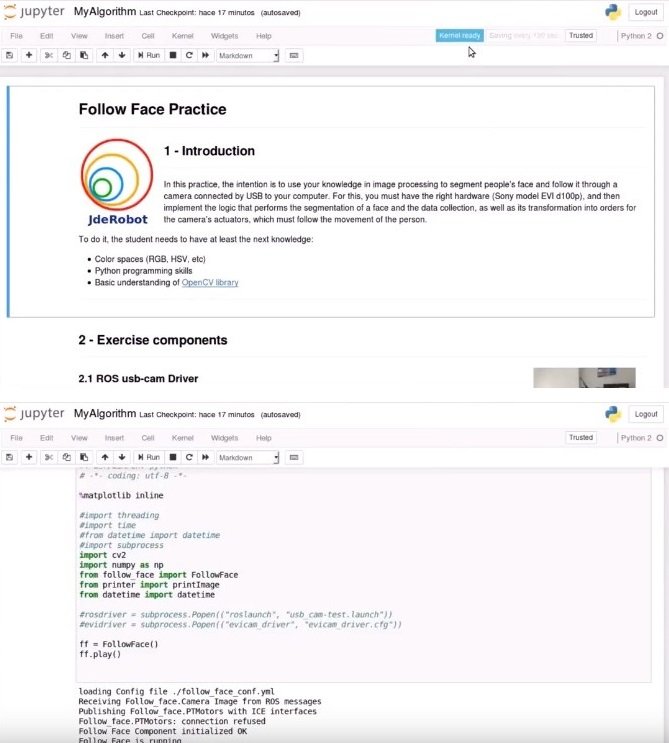
\includegraphics[width=0.98\linewidth]{figures/notebookff.jpg}
		\caption{Notebook Follow Face}
		\label{fig.notebook}
		\end{center}
\end{figure}

Un vídeo demostrando el comportamiento de la práctica a través de Jupyter se puede ver en:

\url{https://www.youtube.com/watch?v=9fOqkw7fUHg}


\lhead[]{CAP\'ITULO \thechapter. LASER LOC}
\chapter{Práctica 2: Autolocalización con Láser}\label{cap.laserloc}
De forma análoga al  \textbf{Capítulo 4}  de este trabajo,  este capítulo recoge el proceso de elaboración y testeo de la segunda práctica creada para el entorno de aprendizaje JdeRobot-Academy. En él, se explicará el soporte que ha sido necesario para su infraestructura, las distintas formas de comunicación que emplea, las características de simulación bajo las que se ha creado la práctica, el componente académico y la solución de referencia.

\section{Enunciado} \label{sec.enunciado}
El objetivo de ésta práctica es que el alumno entre en contacto con uno de los problemas clásicos de la robótica moderna: la auto-localización. En muchos casos, es necesario para que un robot desempeñe la tarea para la que está programado que conozca en todo momento su posición. Si conocemos de antemano el entorno que va a rodear al robot, no existe problema alguno, pues se puede incluir en el programa controlado un código minucioso que le permita conocerlo. Sin embargo, ¿qué hacer si se desea que el robot pueda trabajar en cualquier entorno?

Este problema se resuelve empleando uno de los diversos algoritmos de auto-localización existentes, pero, en concreto, se trata de emplear el método de Montecarlo del filtro de partículas, para que el robot sea capaz en todo momento de saber dónde está con el mínimo error de posición posible. Para ello, se usará un robot aspiradora \textit{Roomba} que incorpora únicamente un sensor láser y un sensor de odometría, además de motores para poder efectuar movimientos en cualquier dirección. 

Con lo anterior, el estudiante deberá programar un algoritmo de auto-localización que permita a la aspiradora estimar su posición en un mundo del cual sólo se proporciona un mapa binario en escala. Para ello, el interfaz gráfico (GUI) de esta práctica incluye distintos \textit{widgets} que facilitan la depuración, con espacios reservados para una visualización adaptada de las lecturas del sensor láser y el propio mapa del entorno, donde se marcarán en todo momento la posición del robot en el mundo, las estimaciones que se van obteniendo y otros componentes elementales que van surgiendo como \textit{output} del algoritmo mencionado. 

En este caso, el algoritmo, también responde a un control reactivo que en cada instante usará  los datos proporcionados por los sensores y sus propias variables internas para actuar adecuadamente en función de la lógica programada. El control reactivo permitirá establecer en todo momento el movimiento del robot, los distintos elementos representables en el GUI y enviar órdenes o salidas que sirvan como respuesta ante cualquier situación.

\section{Infraestructura}
En este apartado se describirá el soporte que sostiene la práctica “Auto-Localización con Láser”. Se comenzará describiendo el modelo de robot empleado, así como los sensores y actuadores que posee. Después, los entornos simulados y sus condiciones serán descritos, de vital importancia para la práctica.

\subsection{Modelo \textit{Roomba}}
El robot en el que se ha inspirado esta práctica es el la aspiradora autónoma modelo \textit{Roomba} de la serie 500, que fue comercializado por la empresa iRobot. Esta aspiradora robótica está equipada con sensores varios con los que sacar conclusiones a partir del entorno y actuadores que le permiten moverse adecuadamente por el escenario. Los dispositivos \textit{Roomba} de esta serie en concreto poseen sensores infrarrojos, un sensor detector de suciedad, un sensor detector de desniveles, y cuentan además con un \textit{bumper}. Sin embargo, no todos serán necesarios para abordar la tarea de auto-localización. Aunque algunos de los sensores  innecesarios seguirán estando disponibles en el modelo, para la práctica se ha empleado modelo de \textit{Roomba} de JdeRobot, que no tiene detector de desniveles debido a que el escenario de nuestra práctica no los contiene (no hay escaleras o cabios de nivel entre habitaciones); y tampoco tiene detector de suciedad, puesto que no es necesario. El objetivo de la práctica era hacer énfasis en el algoritmo de navegación, de manera que de los sensores restantes sólo se usarán el de odometría, para detectar el número de veces que giran las ruedas y el láser, para medir distancias a los obstáculos; ambos detallados más adelante. 

El robot \textit{Roomba} de la serie 500 posee una anchura de 340 milímetros, 92 milímetros de altura, y un peso de 3.6 kg. El modelo Roomba de JdeRobot mide aproximadamente 330 mm de ancho, 90 mm de altura, y un peso de 2.5 kg (\textbf{Figura 5.1}).

\begin{figure}[H]
  \begin{center}
    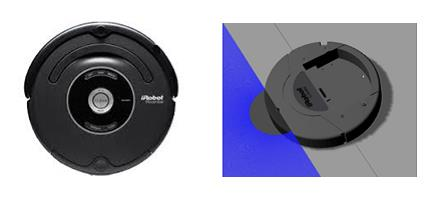
\includegraphics[width=0.85\textwidth, height=5.5cm]{figures/roomba.jpg}
		\caption{Modelo Roomba}
		\label{fig.roomba}
		\end{center}
\end{figure}

Para poder acceder a la funcionalidad que ofrece, se han utilizado tres \textit{plugins} que ejercen de drivers de la aspiradora:

\begin{itemize}
	\item \textit{pose3di}: Los componentes harán uso de este \textit{plugin} para obtener su posición en tiempo real, sólo se empleará la odometría.
	\item \textit{motorsi}: Este \textit{plugin} interactúa con el componente, dotándole de velocidad, ya sea velocidad de tracción o de rotación.
	\item \textit{Laseri}: Este \textit{plugin} será usado por los componentes para obtener información de la distancia entre él y los obstáculos dentro de un sector. 
\end{itemize}

Cabe mencionar en este punto que este robot no ha sido el único modelo empleado. En vistas a añadir mejoras a la práctica, se detallará en \textbf{5.4} el empleo de interfaces \textit{ROS Messages} para la interacción con el robot, para lo cual se ha utilizado una combinación de modelos que incluye el paquete \textit{ros-kinetic} basada en la versión americana de \textit{Roomba}, el robot \textit{Create}, y un modelo conocido de sensor láser como es \textit{Hokuyo}. Reservamos el resto de información relevante para dicho apartado, ya que la solución principal empleará el robot \textit{Roomba}.

\subsubsection{Sensor láser}
En la parte frontal del robot se ha modelado un sensor láser que se utilizará en todo momento en la práctica, por lo que constituye el sensor más importante a estos efectos. 

Está compuesto por un \textit{array} de 180 medidas, que puede medir distancia alrededor de 180 grados en milímetros, con precisión de 1 grado. Su funcionamiento se basa en emitir rayos láser en todas estas orientaciones, que rebotan sobre los objetos existentes (si los hay) de manera no especular, de tal manera que al recibir el rayo devuelto se calcula la distancia al objeto según el tiempo de vuelo.

Una vez más la plataforma JdeRobot encapsula la complejidad de este sensor y su API de utilización. Únicamente se ha construido un \textit{parser} para la práctica que agrupa los datos en forma de \textit{array} de 180 distancias, donde el índice es el ángulo de proyección del haz del láser.
 
\subsubsection{Sensor Odométrico}
En ésta práctica jugará un papel importante el saber cuánto se ha desplazado el robot en un intervalo, dado que servirá para desechar o evolucionar datos involucrados en el algoritmo de auto-localización que explicaremos en \textbf{5.5.1}. Ésta es precisamente la función de la odometría: el uso de sensores de movimiento para determinar el cambio de posición del robot en relación con una posición conocida. Si el robot conoce el diámetro de sus ruedas, simplemente le basta con contar el número de revoluciones de las mismas para determinar qué tan lejos ha viajado. Normalmente, el conteo de vueltas se realiza a través de \textit{encoders}, que emiten un número fijo de pulsos por revolución, siendo éstos los registrados por el software.

Así, el sentido de giro y el número de vueltas que da cada rueda nos ayudará a saber en qué dirección se ha movido el robot, y cuánta distancia ha recorrido.

\subsection{Modelo Asymmetric-Easy-To-Model} 
Dado que la aspiradora necesita un entorno acotado para poder determinar su localización (el láser tiene un alcance limitado), ha sido necesario crear un modelo para que la aspiradora navegue en ella.
Hemos partido del diseño \textit{house\_int2} que utiliza la práctica \textit{Vacuum Cleaner} de JdeRobot-Academy como punto de partida. Este modelo se puede ver en la \textbf{Figura 5.2}:

\begin{figure}[H]
  \begin{center}
    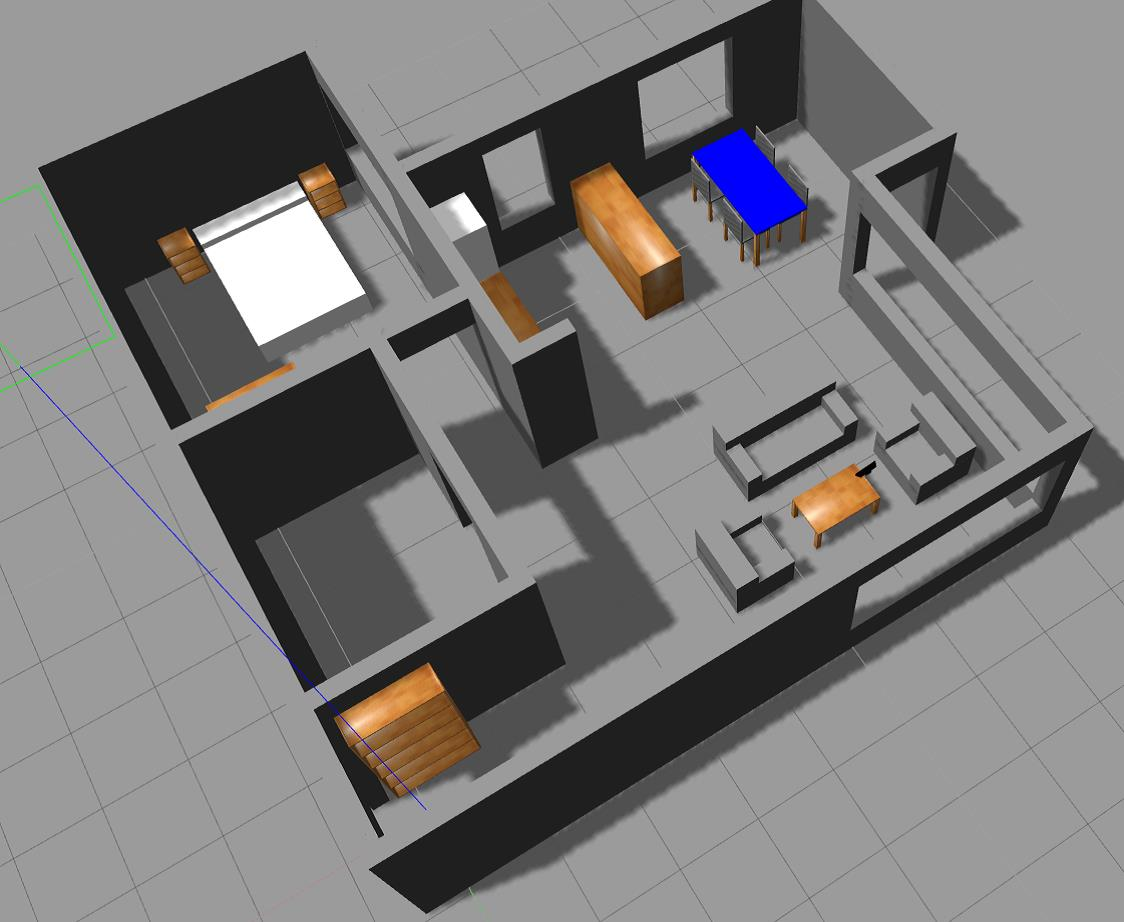
\includegraphics[width=0.75\textwidth]{figures/houseint.jpg}
		\caption{Modelo house\_int2}
		\label{fig.houseint}
		\end{center}
\end{figure}

Las razones bajo la elección de este modelo son:

\begin{itemize}
	\item[--] Entorno acotado por paredes, ideal para obtener lecturas del sensor láser representativas.
	\item[--]	Abundantes obstáculos, lo cual favorece la diferencia entre lecturas en cada punto de la casa.
	\item[--]	Malla de colisiones bien definida, importante cuando se quiere que el robot navegue por la casa sin la aparición de sucesos extraños, como objetos voladores al colisionar con ellos. 
\end{itemize}

Aún con todo ello, este modelo emplea elementos de difícil modelado en una imagen 2D (necesaria para establecer el mapa del mundo), como puede ser la mesa y las sillas: cada pata debía tener el tamaño exacto a escala y estar en la posición adecuada para no obtener procesados erróneos. La zona bajo la cama también resultó un problema. 

Dadas las múltiples ventajas que presenta, se ha creado un nuevo modelo, basado en el anterior, que sustituye todos los elementos difíciles de modelar por paredes, claramente definidas y representadas, mucho más fáciles de modelas en una imagen. Al nuevo mundo que incluía este modelo y el modelo de aspiradora se le ha llamado \textit{Asymmetric-Easy-To-Model.world} (\textbf{Figura 5.3}):

\begin{figure}[H]
  \begin{center}
    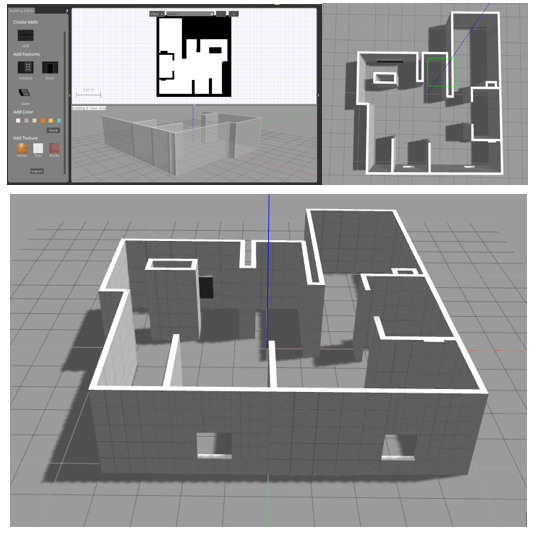
\includegraphics[width=0.95\textwidth, height=12cm]{figures/modeloasymmetric.png}
		\caption{Modelo Asymmetric-Easy-To-Model}
		\label{fig.modeloasymmetric}
		\end{center}
\end{figure}

Como se puede ver, el mundo conserva su forma asimétrica (distintas formas son observadas por el robot en cada orientación y posición) pero está caracterizado por un modelado mucho más simple. 

\subsection{Modelo Choso}
El modelo anterior es el caso más común en el que nos encontramos con el problema de la auto-localización, dada la naturaleza asimétrica del entorno que nos rodea. No obstante, también existen lugares no tan cambiantes, donde las formas se repiten o las superficies límite son iguales o similares en distintas orientaciones. Es por eso que hemos decidido crear el mundo de Gazebo \textit{Choso.world}, el cual es una habitación cuadrada con sólo dos elementos, que ocupan muy poco espacio y por tanto pasan desapercibidos en la mayoría de casos. Este modelo se puede ver en la siguiente imagen (\textbf{Figura 5.4}):

\begin{figure}[H]
  \begin{center}
    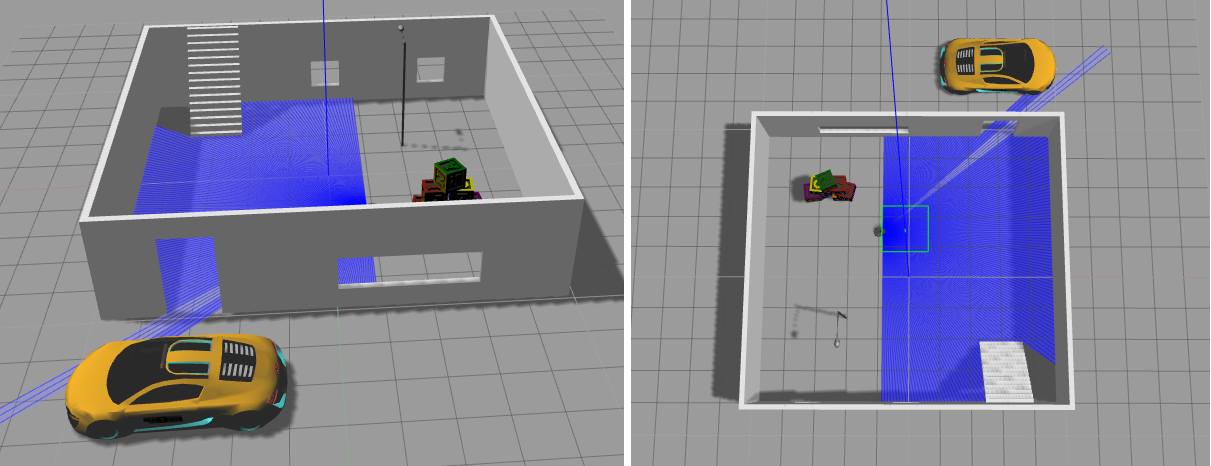
\includegraphics[width=0.96\textwidth]{figures/chosoworld.png}
		\caption{Modelo Choso}
		\label{fig.choso}
		\end{center}
\end{figure}

Introduciremos al robot en este modelo creando un mundo simétrico con fines de experimentación y verificación del comportamiento del algoritmo.

\subsection{Mundo de Gazebo}
A partir de este punto, y a no ser que se indique explícitamente lo contrario, cuando se hable del mundo empleado se asumirá que el modelo empleado es \textit{Asymmetric-Easy-To-Model}.

Así, incorporando los dos modelos involucrados (\textit{Asymmetric-Easy-To-Model} y \textit{Roomba}) y algunas fuentes de luz como el sol, luz ambiente y algunas sombras, se crea el mundo principal en el que abordar la práctica: \textit{Asymmetric-Easy-To-Model.world}(\textbf{Figura 5.5}). Debido a la extensión del fichero de descripción del mundo, sólo incluimos a continuación una parte del mismo para observar su aspecto:

\begin{figure}[H]
  \begin{center}
    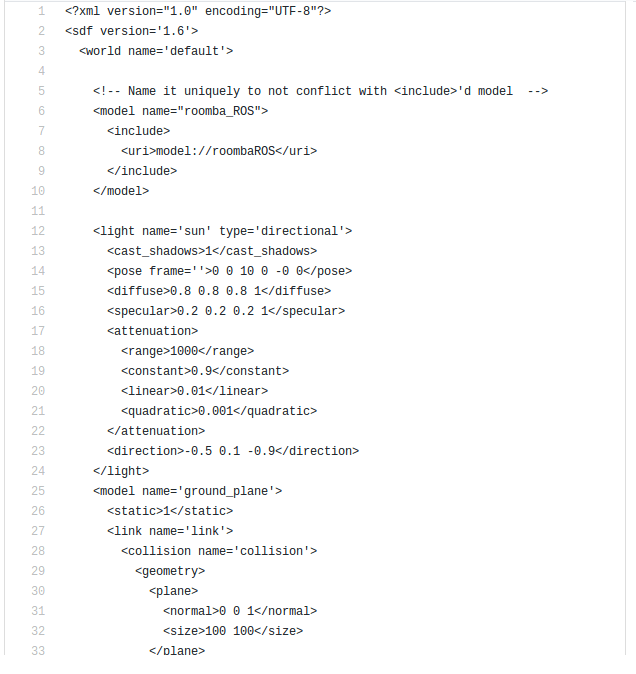
\includegraphics[width=0.98\textwidth]{figures/codeworld.png}
		\caption{Código del mundo}
		\label{fig.codeworld}
		\end{center}
\end{figure}

En él, se puede ver la combinación del modelo re robot creado y de los parámetros de física, aspecto, iluminación y posición que componen el mundo.

\section{Componente Académico}
El componente académico que se ha preparado para esta práctica recoge toda la funcionalidad para ayudar al alumno a enfrentarse a ella y resolverla con éxito. Estas son las piezas que conforman el componente y que quedan resueltas a través de él:  

\begin{enumerate}[label=\alph*)]
	\item Ofrece una interfaz gráfica al usuario que le ayuda a depurar su código; 
	\item Ofrece acceso a todas las interfaces que el robot posee, tanto sensores como actuadores, en forma de métodos simples (oculta el \textit{middleware} de comunicaciones); 
	\item Incluye código auxiliar, como \textit{parsers} o constructores de objetos, que no son parte del algoritmo a realizar, sino que sólo sirven de ayuda para hacer la tarea algo más sencilla.
\end{enumerate}

El componente pone la base que el estudiante culmina incluyendo su código en el método \textit{execute} del fichero \textit{MyAlgorithm.py}, siempre realizando las pruebas que considere oportuno para pulir su solución.

El nodo ofrece un API de sensores y actuadores al programador, además de un API específico para la práctica en el que se encontrarán otros métodos e incluso variables disponibles para facilitar la tarea. En cuanto al API del robot, tenemos:

\begin{itemize}
	\item \textit{self.sensors.motors.sendVelocities(vel)}: Para enviar comandos de velocidad a través de:
    \begin{itemize}[label={$\diamond$}]
			\item \textit{vel = CMDVel()}: constructor de comandos de velocidad
       \item \textit{vel.vx = valor}: velocidad lineal
       \item \textit{vel.az = valor}: velocidad angular
    \end{itemize}
    \item \textit{self.sensors.laserdata} o \textit{self.gui.getLaserData()}: dos posibilidades equivalentes para obtener los datos láser.
    \item \textit{self.parse\_laser\_data(laser)}: Para transformar los datos láser en una estructura más fácilmente manejable.
		\item \textit{self.pose3d.getPose3d().x}, \textit{self.pose3d.getPose3d().y}, \textit{self.pose3d.getPose3d().yaw}: para obtener los datos de posición y orientación del robot.
\end{itemize}

Por otro lado, la manera de utilizar la funcionalidad que este nodo ofrece resuelta es:

\begin{itemize}
	\item ||\textbf{Clase Particle}||: \textit{Particle(x, y, yaw, prob, self.map.robotAngle)}: Constructor de partículas.
	\item \textit{self.setParticles([p1,p2,p3,...])}: Representa una lista de partículas en el GUI.
	\item \textit{self.setEstimation(particle)}: Para mostrar una estimación en el interfaz
	\item \textit{img = self.map.pixmap.toImage()}: para obtener la imagen (mapa) del interfaz.
	\item \textit{self.paintTheoricalLaser(theoricalLaser)}: para representar un láser en la interfaz.
	\item \textbf{(variable)} \textit{self.particleClicked}: almacena la última partícula sobra la que se ha hecho click en el GUI. 
	\item \textit{self.map.map2pixel((x,y))}: obtiene el pixel correspondiente a las coordenadas (x,y).
	\item \textit{self.map.pixel2map((px,py)}: obtiene las coordenadas reales asociadas al pixel [px,py] del mapa.
\end{itemize}

Con ello, todo lo necesario queda a disposición del alumno para comenzar la tarea. El único componente externo que el nodo académico necesita es un fichero de configuración que recoja los \textit{endpoints} que las interfaces de los sensores y actuadores descritos en \textbf{5.2.1}, \textbf{5.2.1.1} y \textbf{5.2.1.2} utilizan para publicar la información o recibirla del nodo. Este archivo tiene extensión \textit{.yml}, lo cual implica que debe cumplir las especificaciones del formato de serialización de datos YAML. Para esta práctica en concreto, añadimos además la configuración necesaria para establecer el mapa binario de referencia del robot. Tiene el siguiente aspecto(\textbf{Figura 5.6}):

\begin{figure}[H]
  \begin{center}
    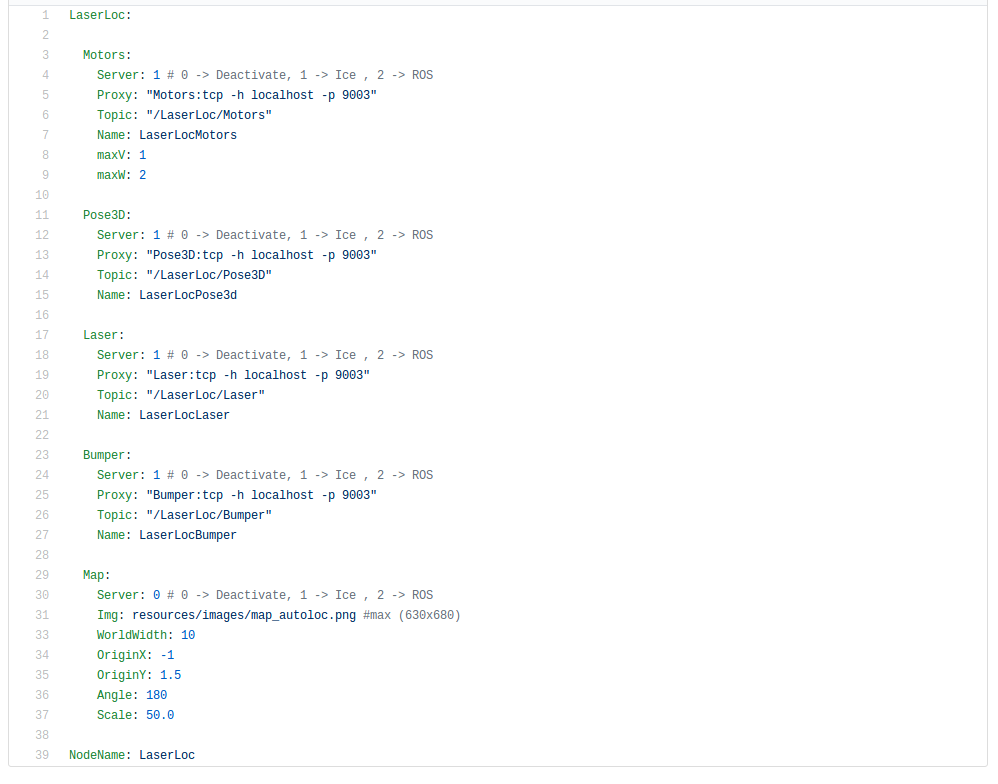
\includegraphics[width=0.98\textwidth]{figures/ymlantiguo.png}
		\caption{Fichero de configuración YAML de LaserLoc}
		\label{fig.llyaml}
		\end{center}
\end{figure}

En la versión básica, todas las comunicaciones se realizarán a través de ICE, a falta de \textit{plugins} que administren los sensores y actuadores a través de \textit{ROS Messages}. Otra versión de la práctica utilizando estos interfaces será descrita en \textbf{5.4}, demostrando que JdeRobot es totalmente compatible con ROS, únicamente retocando en este fichero de configuración el \textit{flag} que indica si el servidor de datos es uno u otro. Además, vemos que la información del mapa cuenta con atributos como el tamaño, la escala o el \textit{path} que conduce a la imagen binaria. Por último, se establecen las velocidades máximas de tracción y rotación en base a las necesidades de la práctica. Cabe mencionar que gracias a la configuración interna de la plataforma JdeRobot es posible que las distintas interfaces utilicen un mismo puerto.

El componente se ha segmentado en distintos hilos para favorecer la simultaneidad de ejecución de distintas tareas clave. En un principio, el componente sólo contaba con dos hilos básicos de ejecución:

\begin{itemize}
  \renewcommand{\labelitemi}{$\to$}
	\item Hilo de algoritmo: se encarga del refresco de la ejecución del algoritmo, ya que este se ejecuta de modo iterativo o cíclico. El tiempo de refresco es importante, dado que el algoritmo necesario para solventar la práctica es bastante sensible a pequeños cambios en las lecturas, que deben desencadenar correcciones en la ejecución. Por ello, el tiempo de refresco es de 10 ms.
	\item Hilo de la interfaz gráfica de usuario (GUI): Este hilo es el encargado de actualizar la interfaz gráfica y los \textit{widgets} incorporados en ella. El intervalo de actualización de la interfaz debe ser pequeño, de tal manera que los cambios en los sensores o en el mapa puedan ser representados en tiempo real. Por ello, se ha fijado el tiempo de refresco a 20 ms.
\end{itemize}

Estos agilizaban la respuesta de los distintos módulos implicados. Sin embargo, se hizo necesario añadir un tercer hilo de ejecución:

\begin{itemize}
  \renewcommand{\labelitemi}{$\to$}
	\item Hilo de sensores: el tercer hilo se ha añadido para actualizar los datos de los sensores y los actuadores a través de las interfaces que correspondan (ICE o ROS). El tiempo de refresco de este hilo es muy importante, dado que un intervalo largo radicaría en lecturas desactualizadas de los sensores. Por ello, dicho tiempo también se ha fijado en 20 ms.
\end{itemize}

Esto se debe a la sobrecarga aritmética que el algoritmo de localización introduce en el componente. Entraremos más en detalle sobre esta decisión en \textbf{5.5.2}.

Con todo ello, el nodo dispone la interfaz de usuario con algunos elementos de depuración (accesibles a través del API descrito más arriba) para que el usuario se centre en el algoritmo a escribir. La manera de integrar dicho algoritmo en el nodo para que llegue al robot también es tarea del componente académico, por lo cual se reserva un espacio concreto para que el alumno inserte la lógica, debidamente indicado en el fichero de instrucciones incluido (\textit{README.md}).

\subsection{Interfaz gráfica}
La interfaz gráfica de usuario (GUI) se emplea para representar información que pueda ayudar a resolver el algoritmo planteado, lo cual resultará vital en el camino hacia la resolución de la misma. Se ha construido a través de PyQt5, y se encargará de mostrar la salida de la ejecución del algoritmo en cada instante, ideal para depurar y observar su evolución.

\begin{figure}[H]
  \begin{center}
    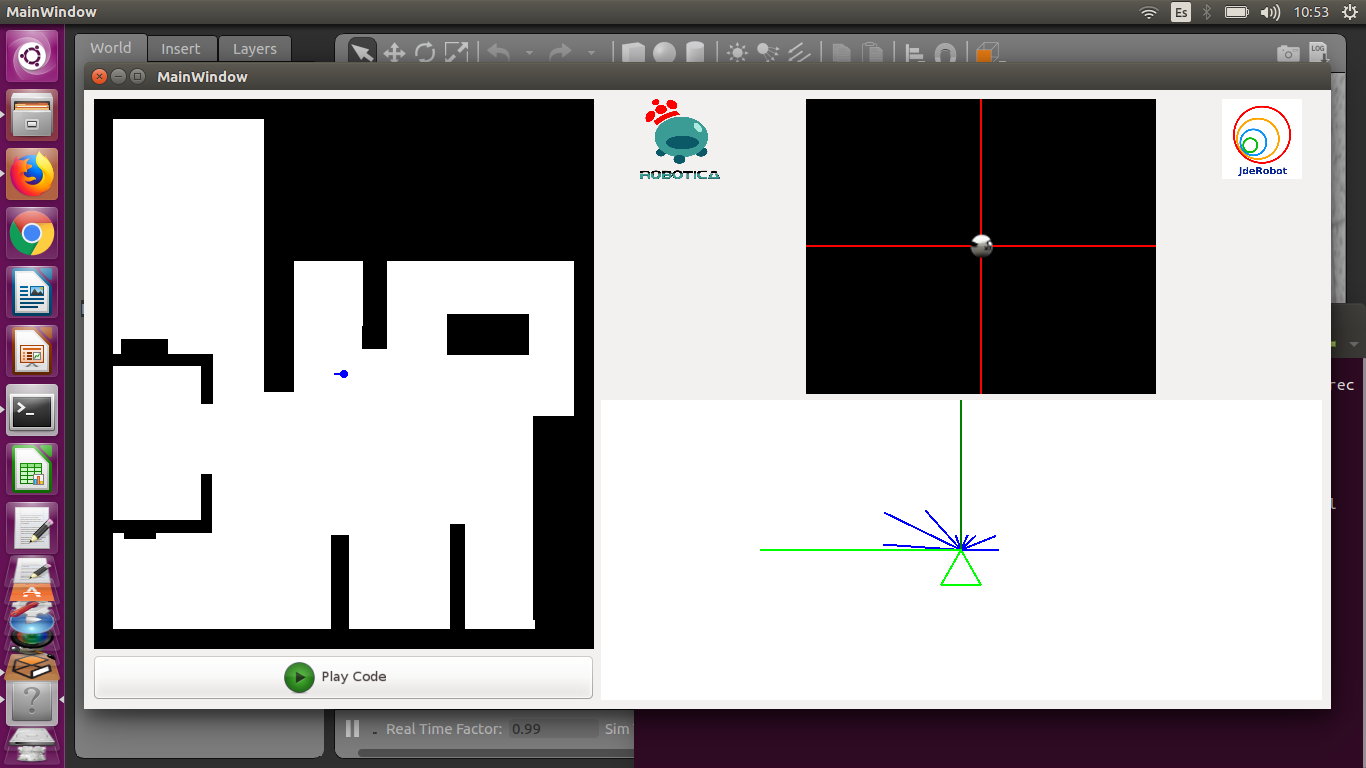
\includegraphics[width=0.98\textwidth]{figures/llgui.png}
		\caption{Interfaz Gráfica Laser Loc}
		\label{fig.llgui}
		\end{center}
\end{figure}

Esta GUI (\textbf{Figura 5.7}) está formada por 3 \textit{widgets} para el control y visionado del comportamiento del robot. El primero de ellos, situado a la izquierda, es quizás el más importante, pues muestra al programador un mapa binario que el robot utiliza para poder realizar cálculos pertinentes para llevar a cabo su auto-localización, pero con información gráfica con la que este no cuenta: las sucesivas generaciones de partículas (información ampliada en \textbf{5.3.3.1}) que surgen del algoritmo evolutivo que se ha de usar, el cual comentaremos en \textbf{5.5}. Así, en el mapa se ven reflejados los obstáculos (zonas negras), las zonas libres (espacio en blanco), la posición y orientación del robot en el espacio dado (a través de un punto azul), la evolución de las partículas e incluso las trayectorias (ver \textbf{5.3.3} para más detalles). 
El segundo de los elementos del interfaz, situado en la parte superior derecha es el clásico teleoperador, el cual se incorpora en todas las prácticas para añadir la capacidad de controlar la posición del robot y su rotación a través de órdenes de velocidad lineal y angular. Esto facilita el proceso de depuración y sirve de apoyo en los primeros pasos hacia la solución.

Por último, el espacio inferior derecho se ha reservado para la representación de las lecturas que ofrece el láser del robot en cada momento, y también para graficar de manera aproximada el cálculo de láser teórico que el robot hace de cada partícula (ver \textbf{5.3.2}).

En la parte inferior se ha incluido un botón para ejecutar el algoritmo y pararlo cuando sea necesario, lo cual también para todas las representaciones y el movimiento del robot. 

\subsection{Gráfica de los láseres Real y Teórico}
Como se ha comentado en el punto anterior, uno de los elementos de visualización que incluye la práctica es la posibilidad de ver de forma gráfica los datos que ofrece el sensor láser, así como una representación de los haces láser de cada partícula calculados a partir de la lectura que ofrecería el robot en el caso de que su posición y orientación coincidiesen con los de esta. Así, lo que se representa es lo siguiente:

\begin{enumerate}
	\item \textbf{- Láser Real}
	\begin{figure}[H]
		\begin{center}
			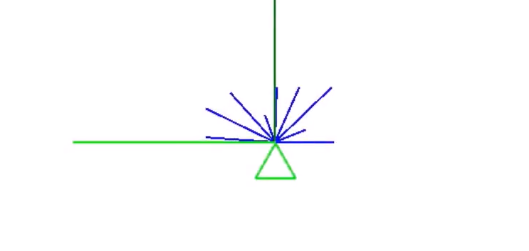
\includegraphics[width=0.65\textwidth]{figures/laserreal.png}
			\caption{Laser Real}
			\label{fig.laserreal}
			\end{center}
	\end{figure}
Dado que las lecturas utilizadas para esta práctica están formadas por 9 haces en total (uno cada 20º con respecto a la normal de la orientación del robot), lo que se representa es un conjunto de segmentos cuya longitud se corresponde con la distancia (a escala 50:1) al primer obstáculo en la dirección marcada por el ángulo del haz (\textbf{Figura 5.8}). Como se dijo en \textbf{5.2.1.1}¸ las medidas del láser constan de 180 pares de valores, y su reducción a los 9 utilizados se describirá en \textbf{5.5.2}. Los datos de \textit{parsean} convenientemente antes de ser representados, y la representación es en todo caso absoluta (no tiene en cuenta la orientación del robot, ya que en caso contrario la resolución de la práctica sería una tarea mucho más sencilla).
\item \textbf{- Láser Teórico}
	\begin{figure}[H]
		\begin{center}
			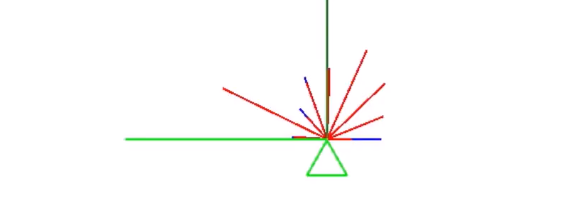
\includegraphics[width=0.65\textwidth]{figures/laserteorico.png}
			\caption{Laser Teórico}
			\label{fig.laserteorico}
			\end{center}
	\end{figure}
Como veremos más adelante, para cada partícula involucrada en el algoritmo se deberá calcular un “láser teórico” (\textbf{Figura 5.9}), nombre con el que hemos bautizado a la lectura que se obtendría en el sensor en el supuesto de que el robot ocupase la posición de dicha partícula y compartiese su orientación. Se puede ver que en la representación se muestra la superposición de ambos datos láser: el real en azul y el teórico en rojo, de manera que en todo momento se puede comprobar si una partícula ofrece una lectura similar a la del robot o no. Dado que el algoritmo se compone de muchas partículas, para activar la representación del láser teórico de una partícula determinada bastará con hacer click sobre ella en el \textit{widget} que contiene el mapa de referencia. De nuevo, la representación es absoluta, no relativa a las características de cada partícula.
\end{enumerate}

\subsection{Mapa de Referencia}
El elemento gráfico vital es el mapa que robot utiliza para poder hacer cálculos sobre su entorno. Este mapa es una imagen con sólo dos valores posibles para cada pixel: blanco y negro. Esto facilita las tareas de procesado, ya que se tiene un juego de valores fijo, reducido y conocido. El robot se va a basar en dicho mapa para poder realizar el cálculo de los datos teóricos láser, llevando a cabo un método de trazado de rayos sobre la imagen sobre el que se profundizará en la explicación de la solución. Este mapa emplea una codificación de color para expresar visualmente la probabilidad de cada suceso, como el que se muestra en la \textbf{Figura 5.10}.

\begin{multicols}{2}
\begin{figure}[H]
		\begin{center}
			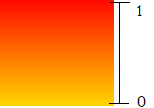
\includegraphics[width=0.3\textwidth]{figures/gradcolor.png}
			\caption{Codificación de color}
			\label{fig.gradcolor}
			\end{center}
	\end{figure}

Así, cada partícula se representará con un color dentro de este rango, en función de sus posibilidades de ser la posición real en la que se encuentra el robot.

Hay dos excepciones para esta codificación de color:
\end{multicols} 

\begin{itemize}
	\item[--] La posición real del robot, también representada en forma de partícula, utilizará un color azul oscuro en todo momento
	\item[--] Las estimaciones que el robot hará de su posición se representarán en azul claro.
\end{itemize}

Por último, este lienzo también superpondrá al mapa la trayectoria que el robot sigue en todo momento representada en negro, y la trayectoria estimada por el robot para localización en movimiento, representada también en azul claro, como se ve en la \textbf{Figura 5.11}:

\begin{figure}[H]
	\begin{center}
		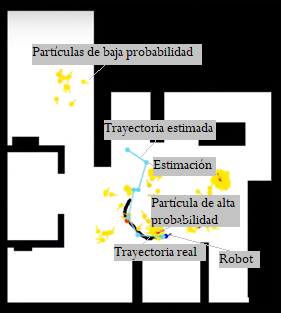
\includegraphics[width=0.5\textwidth]{figures/mapareferencia.png}
		\caption{Mapa de referencia}
		\label{fig.mapareferencia}
		\end{center}
\end{figure}

\subsubsection{Partículas}
El elemento principal en el que se basa el algoritmo que se debe emplear en la solución son las partículas, las cuales ya hemos mencionado en el desarrollo de este capítulo. Lo primero es explicar su composición y características:

Estas partículas no son más que puntos en el espacio en los que el robot se proyecta a sí mismo, es decir, posiciones y orientaciones que el robot puede ocupar y tomar en el escenario. Por ello, cada partícula consta de:

\begin{itemize}
  \renewcommand{\labelitemi}{$\to$}
	\item Un vector de coordenadas (x, y, z) que representa su posición en el espacio. Todas las posiciones ocupadas por algún obstáculo no están disponibles para el robot, de manera que tampoco pueden estarlo para las partículas. La coordenada z se fija siempre a 0, dado que el escenario no contiene desniveles.
	\item Un atributo de orientación, que representa su rotación con respecto al mapa. 
	\item Un valor de probabilidad, que almacena el valor numérico obtenido al comparar el láser de la partícula con la lectura real.
\end{itemize}

A fin de organizar el código, se ofrece al programador la clase \textit{Particle}¸ la cual actúa como constructor de partículas, asociando a cada una sus correspondientes características accesibles como atributos de un objeto Python:

\begin{figure}[H]
	\begin{center}
		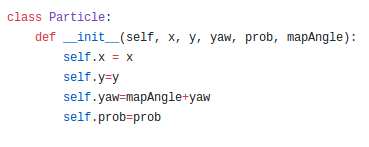
\includegraphics[width=0.6\textwidth]{figures/claseparticle.png}
		\label{fig.claseparticle}
		\end{center}
\end{figure}

\subsubsection{Trayectorias}
En cuanto a las trayectorias que se representan en el gráfico, cabe decir que la ruta real está formada por las últimas 100 posiciones diferentes que ha ocupado el robot para su representación, de manera que se modifica con las sucesivas iteraciones. Sirve como apoyo para pulir el comportamiento del algoritmo, ya que el programador podrá compararla en todo momento con la trayectoria que su lógica implementada va creando. Su representación es automática y se encarga la interfaz del nodo académico.

Por otro lado, la trayectoria estimada es obtenida a través de la unión de las distintas estimaciones de posición que el algoritmo del robot hace a lo largo del tiempo. Se ha dotado al componente con un API para el establecimiento de estimaciones a visualizar en la gráfica:

\hspace{0.32\linewidth} \textit{self.setEstimation([x,y])}

Con lo cual se puede hacer un seguimiento del comportamiento del algoritmo a largo plazo.
 
\section{Comunicaciones con ROS}
A fin de crear la primera práctica auto-contenida del entorno JdeRobot, se utilizará interfaces de ROS para implementar una nueva versión de la práctica que no dependa del paquete de comunicaciones que emplean todas las prácticas de Academy (\textit{JdeRobotComm}), de tal manera que un supuesto usuario futuro sólo tendría que instalar en su máquina el simulador, el paquete \textit{kinetic} de ROS y los interfaces y \textit{plugins} necesarios y los modelos y mundos preparados por el entorno. Con esto, sólo se habría de clonar el repositorio del entorno académico en el cual están las prácticas y empezar a programar, sin la necesidad de instalar otros paquetes necesarios para ejecutar las prácticas actuales del entorno. Dado que ROS tiene soporte en distintas plataformas, se conseguiría tener una práctica totalmente funcional para muchos usuarios diferentes.

\begin{multicols}{2}
	\begin{figure}[H]
	\begin{center}
		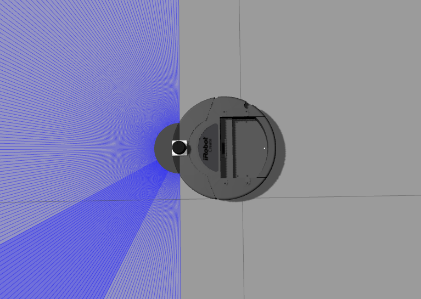
\includegraphics[width=0.3\textwidth]{figures/create.png}
		\caption{Modelo Roomba ROS}
		\label{fig.create}
		\end{center}
\end{figure}

El nuevo robot (\textbf{Figura 5.12}) conserva todas las interfaces de sensores y actuadores anteriores (incluidas aquellas no utilizadas en esta práctica como el \textit{bumper}), por lo que su funcionalidad es equivalente.
\end{multicols}
En cuanto al sensor láser, hemos utilizado un modelo ya creado llamado \textit{hokuyo} (\textbf{Figura 5.13}) que ya se comunica a través de \textit{ROS Messages}, el cual se ha incrustado en la parte frontal del robot.

Para conservar la funcionalidad que ofrecía la aspiradora en la simulación, hemos usado los siguientes \textit{plugins}:

\begin{multicols}{2}
	\begin{figure}[H]
	\begin{center}
		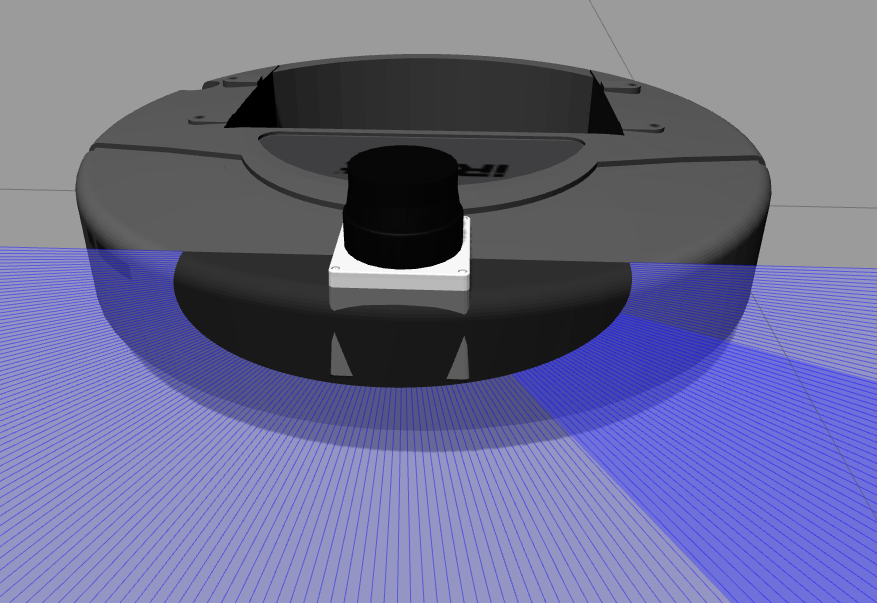
\includegraphics[width=0.3\textwidth]{figures/hokuyo.png}
		\caption{Modelo Hokuyo sobre Roomba}
		\label{fig.hokuyo}
		\end{center}
\end{figure}

\begin{itemize}
	\item \textit{libgazebo\_ros\_bumper.so} 
Para gestionar el sensor bumper
	\item \textit{libgazebo\_ros\_laser.so}  
Para recibir datos del sensor láser
	\item \textit{libgazebo\_ros\_diff\_drive.so } 
Para obtener odometría y controlar motores
\end{itemize}
\end{multicols}

Todos ellos compatibles con la versión \textit{kinetic} de ROS.

Una vez creado el modelo, basta con incluirlo en el mundo del que ya disponíamos para poder usarlo. No obstante, son necesarios unos pequeños cambios en el nodo:

Como ya hemos dicho, perseguíamos una práctica auto-contenida, de manera que el fichero principal del nodo (\textit{laser\_loc.py}) debe ahora incluir todo lo necesario para establecer y mantener la comunicación con el robot, y para realizar la conversión entre los mensajes recibidos y los datos que el nodo puede manejar. 

Por tanto, dicho fichero debe contener:
\begin{enumerate}
	\item El código necesario para conectar con cada nodo del robot, para lo cual se usan sentencias tipo:
	\begin{figure}[H]
	\begin{center}
		
\includegraphics[width=0.75\textwidth]{figures/initnode.png}
		\label{fig.initnode}
		\end{center}
	\end{figure}
	\item La suscripción de cada nodo inicializado a su correspondiente \textit{topic} de ROS, es decir, a su bus de intercambio de mensajes en el cual el driver encargado del control del nodo (ya sea sensor o actuador) publica o recibe mensajes con cierta forma:
	\begin{figure}[H]
	\begin{center}
		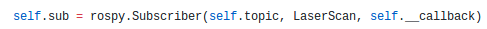
\includegraphics[width=0.75\textwidth]{figures/subscriberlaser.png}
		\label{fig.subscriberlaser}
		\end{center}
	\end{figure}
	\hspace{0.48\linewidth}o
	\begin{figure}[H]
	\begin{center}
		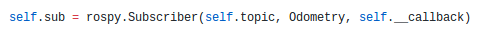
\includegraphics[width=0.75\textwidth]{figures/subscriberodometry.png}
		\label{fig.subscriberodometry}
		\end{center}
	\end{figure}
	\item La transformación de los mensajes que se intercambian por los buses y la utilizada por el nodo de la práctica:
	\begin{figure}[H]
	\begin{center}
		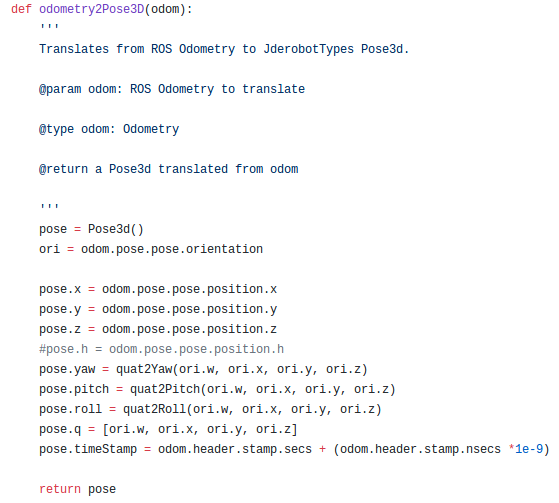
\includegraphics[width=0.60\textwidth]{figures/odom2pose.png}
		\label{fig.odometry2pose}
		\end{center}
	\end{figure}
\end{enumerate}

Para todo ello, el nuevo fichero principal amplía su funcionalidad con una serie de clases que se encargan de la construcción de objetos que tengan en cuenta todas las especificaciones anteriores.
La asociación entre cada nodo y su \textit{topic} se traduce en una serie de cambios en el fichero de configuración (\textbf{Figura 5.14}) que se facilita a la hora de ejecutar:

\begin{figure}[H]
	\begin{center}
		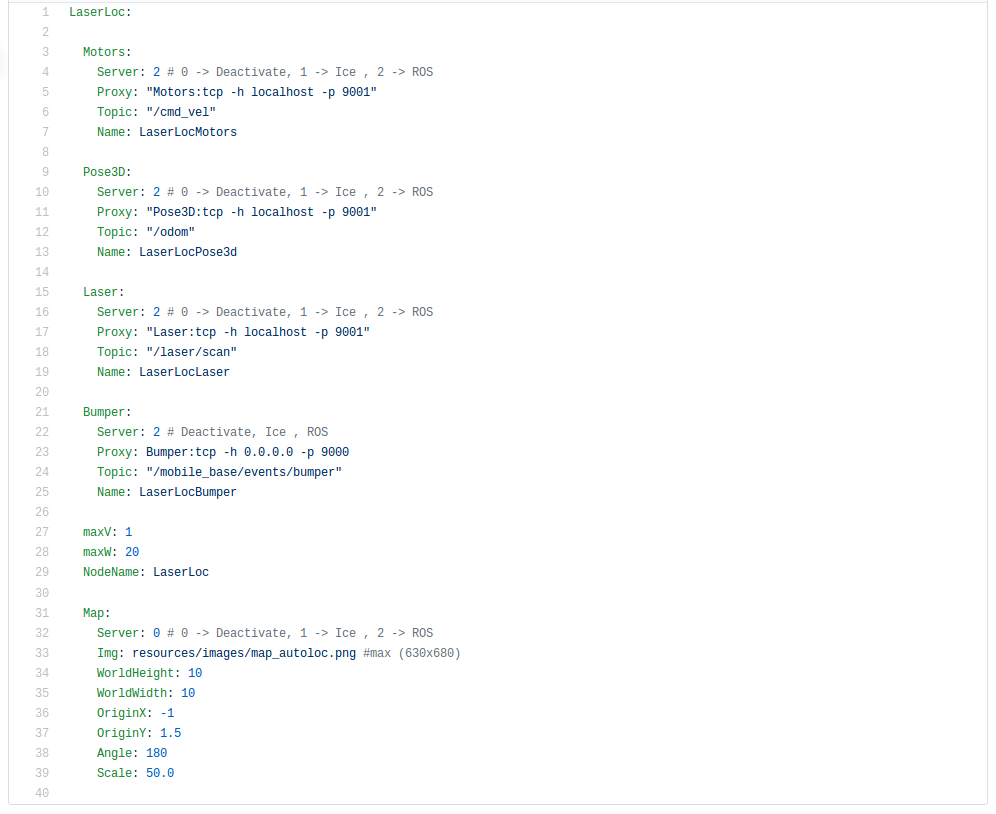
\includegraphics[width=0.98\textwidth]{figures/llymlfinal.png}
		\caption{Fichero de configuración YAML con interfaces de ROS}
		\label{fig.llymlfinal}
		\end{center}
\end{figure}

Por lo demás, y al estar hecho de manera genérica, no son necesarios más cambios en ningún otro componente del nodo gracias a la compatibilidad de JdeRobot con el \textit{middleware}.

\section{Solución de referencia}
Persiguiendo el objetivo de implementar la lógica de auto-localización del robot de esta práctica, la solución ha de contener un algoritmo de procesado de imagen combinado con un algoritmo matemático que permita implementar el filtro de partículas. Para esta práctica no es adecuado incluir también un algoritmo de pilotaje, pues a estos efectos se dispone de un teleoperador, lo que contribuirá a que la ruta seguida por el robot sea en todo caso aleatoria, permitiendo así comprobar las prestaciones del algoritmo reactivo resultante de manera más crítica. 
Comenzaremos esta sección describiendo los distintos tipos de algoritmos de localización existentes, argumentando el porqué del que hemos escogido. Con ello construiremos una solución que se establecerá como solución de referencia en la plataforma, pero que sólo es uno de los muchos posibles métodos con el cual alcanzar el fin. El código quedara recogido en el fichero \textit{MyAlgorithm.py} que para este caso también tiene naturaleza iterativa, de manera que en cada iteración se obtiene datos de los sensores, se procesa y se actúa en consecuencia (se evoluciona el algoritmo). El código a escribir irá de nuevo a parar al método \textit{execute}, el cual debe ejecuta la lógica de manera cíclica en el \textit{thread} de algoritmo y computación.

\subsection{Algoritmos de autolocalización}
El campo de la localización se puede dividir en dos grandes subgrupos: el primero y más sencillo es partir de una posición inicial conocida, en este caso para determinar la posición final del robot habrá que estimar los errores acumulados por los odómetros. El segundo y más difícil aborda lo que se conoce como localización global, en la que se desconoce la posición inicial del robot y los errores son mayores que en el caso anterior, ya que en este caso hay más fuentes que los introducen. Nosotros pretendemos abordar precisamente este segundo caso, para el cual hay que tener en cuenta varios parámetros cambiantes que a su vez hacen que cambien el problema y la solución.
Es por eso que las distintas maneras de abordar el problema se gradúan en base a su dificultad, dependiendo por ejemplo en el tipo de láser utilizado, ya que emplear sensores de posición facilita en gran medida la localización (como mucho habrá que estimar y corregir los errores o derivas del sensor) u otros equivalentes como sensores GPS (en exteriores) o localización geométrica a través de balizas. Sin embargo, la versión más difícil y elaborada del problema de la localización, es enfrentarse a ella usando sensores no específicos de posición (láser, cámaras,..). En este caso la información de posición se obtiene relacionando las lecturas sensoriales con el mapa del entorno.
Existen diferentes técnicas como el \textit{scan maching} que se basa en ir “superponiendo” lecturas del mapa local sobre el global intentado ajustar las lecturas a este último, pero no es apta para localización global. Otra técnica buena para la localización local son los filtros de Kalman, un filtro de Bayes recursivo que estima la distribución a posteriori del estado de un sistema condicionada en función de los datos. Su principal limitación es que se trata de una técnica unimodal y exclusivamente gaussiana [Isard y Blake, 1998]. 
Es así como llegamos a la localización probabilística, una de las mejores técnicas para localización en interiores. La idea principal de este método es crear un modelo capaz de estimar la probabilidad de estar en una posición del escenario basándose sólo en información extraída a partir de la asunción de que se está en esa posición. Comparando dicha información con la que se obtiene de los sensores en la posición real se llega al valor de la probabilidad de que el robot ocupe esa posición teórica. Esa estimación de posición se actualiza con la incorporación de nuevas observaciones y movimientos, lo cual encaja a la perfección con nuestra estructura cíclica para la práctica. El inconveniente de esta técnica es que almacena la probabilidad para todas las posibles posiciones, lo que hace que sea lenta y no escalable a grandes entornos donde el número de posiciones posibles es muy grande. Esto se tratará adecuadamente en \textbf{5.5.2}. Precisamente por este inconveniente surgen nuevas técnicas basadas en lo anterior como el filtro de partículas, el cual vamos a emplear, que consiste en mantener un conjunto muestral de posibles posiciones y calcular la probabilidad de cada una. Mediante remuestreo estadístico, estas posiciones acaban convergiendo hacia la posición correcta del robot. El número reducido de muestras (comparado con el de la localización probabilística) hace que se minimicen los costes computacionales y que el algoritmo sea escalable a grandes entornos. Se trata de un filtro bayesiano recursivo en el que el conjunto de muestras
\begin{equation}
\{x_{i},P(x_{i})\}, i = 1..n,
\end{equation} estaría formado por coordenadas de posición y orientación
\begin{equation}
x_{i} = (x, y, \theta),
\end{equation} inicialmente escogidas al azar sobre el escenario, que emplea su probabilidad P(xi) calculada a partir de lecturas del sensor láser comparadas con medidas efectuadas sobre el mapa en función de estas coordenadas de posición y de un modelo de observación para ir seleccionando aquellas posiciones más probables.

El filtro de partículas pertenece a la familia de técnicas de Monte Carlo, un conjunto de métodos probabilísticos de remuestreo desarrollados entre los años 1945 y 1955 para el campo de la física. En este contexto, cada muestra se denomina “partícula”, y el objetivo es conseguir que la nube o generación de partículas establecidas de modo aleatorio converja en la posición real del robot. Inicialmente la población de partículas se distribuye uniformemente en $(x,y, \theta)$ sobre todo el mundo, y en cada iteración del algoritmo se evoluciona a una nueva población a partir de la anterior, la cual está formada por “hijos” de partículas que tenían alta probabilidad en dicha población anterior. El algoritmo se realiza en tres pasos que se ejecutan siempre y de forma iterativa:

\begin{itemize}
	\item \textbf{ Modelo de movimiento}: se desplazan las muestras $(\Delta r, \Delta\theta)$, equivalente al desplazamiento efectuado por el robot desde la última vez que se incorporó el movimiento del mismo. Esto se traduce en que el método de localización permite incorporar información de desplazamiento si se dispone de ella para generar conjuntos sucesivos de partículas de mejor calidad. 
	\item \textbf{Modelo de observación}: se calculan las nuevas probabilidades de todas las muestras a partir de la lectura del sensor láser. Se ha de ajustar una función de salud que se encargue de asociar probabilidades altas a aquellas zonas compatibles con la lectura láser real y bajar la de las zonas incompatibles. 
	\item \textbf{Remuestreo}: se genera una nueva población a partir de la anterior siguiendo el algoritmo de la ruleta (\textbf{Figura 5.15}), que consiste en girar la ruleta tantas veces como hijos queremos generar. Cada partícula tiene un sector proporcional a su probabilidad en la ruleta, de manera que si el valor está incluido en el sector de una partícula concreta, esta genera un hijo “idéntico” en la siguiente población.
\end{itemize}

\begin{figure}[H]
	\begin{center}
		\includegraphics[width=0.3\textwidth]{figures/ruleta.png}
		\caption{Algoritmo de la Ruleta}
		\label{fig.ruleta}
		\end{center}
\end{figure}

Debajo de este modelo existen muchos parámetros relevantes para la implementación, de manera que entraremos un poco más en detalle: 
Se ha dicho que se debe disponer de un modelo de observación capaz de calcular las medidas láser de forma teórica de cada partícula y asociarles una probabilidad.

\begin{multicols}{2}
	\begin{figure}[H]
	\begin{center}
		\includegraphics[width=0.4\textwidth]{figures/modeloobsv.png}
		\caption{Ejemplo de modelo de observación}
		\label{fig.modeloobsv}
		\end{center}
	\end{figure}
La Figura de la izquierda (\textbf{Figura 5.16}) muestra un ejemplo de este modelo, en el cual las partículas más lejanas a la posición del robot y en distinta orientación toman valores más bajos de probabilidad representados con un color más claro (amarillo), mientras que las cercanas a la posición real toman un valor más alto, representado en un color intenso (rojo). El cálculo del “láser teórico” es lo que permite asignar a cada una su probabilidad. Para obtenerlo, emplearemos un algoritmo de trazado de rayos sobre el mapa, que básicamente se basará en trazar
\end{multicols} una línea recta en el espacio bidimensional euclidiano desde la posición de cada partícula en la imagen hasta el punto donde se encuentre el máximo de distancia que puede abarcar el láser en las 9 direcciones que deben componer la lectura láser. En esta recta se va comprobando cada cierta distancia (paso $\lambda$) si el color del píxel es blanco (espacio libre) o negro(obstáculo), en cuyo caso se obtiene el punto en el que rebotaría el haz láser. Con ello, y conociendo la escala del mapa dado, obtenemos una distancia equivalente en la imagen para cada haz a la que se obtendría en el mundo si el robot ocupase esa posición. Así, 
\begin{equation}
X_{obstaculo} = (PX_{partícula} + \lambda*cos(\alpha_{haz}))*escala
\end{equation}
\begin{equation}
Y_{obstaculo} = (PY_{partícula} + \lambda*sin(\alpha_{haz}))*escala
\end{equation}
\begin{equation}
Distancia = \sqrt{(X_{obstaculo}-X_{partícula})^2+(Y_{obstaculo}-Y_{partícula})^2}
\end{equation}

Con esta distancia de cada haz, basta con compararla con la distancia que marca el sensor real en dicha orientación, con lo cual se obtendrá un error (error = LaserReal- LaserTeórico). Sólo es necesario acumular este error en cada orientación para asignar posteriormente una probabilidad. Cuanto menor error, las lecturas son más parecidas y se asignará la mayor probabilidad.

Por otro lado, el modelo de movimiento es de gran importancia para descartar información inservible y revalidar información adecuada. Se trata de incorporar el movimiento del robot a la generación de partículas en coordenadas polares $(\Delta r, \Delta\theta)$, para lo cual: 

\begin{equation}
\Delta x = x_{t+1} - x_{t}
\end{equation}
\begin{equation}
\Delta y = y_{t+1} - y_{t}
\end{equation}
\begin{equation}
\Delta\theta = \theta_{t} - \theta_{t-1}
\end{equation}
\begin{equation}
\Delta r = \sqrt{(\Delta x)^2+(\Delta y)^2}
\end{equation}

Bastará con sumar el incremento a la posición de cada partícula. Sin embargo, esta suma ha de ser consecuente con la orientación de la partícula (\textbf{Figura 5.17}), o más en concreto con el ángulo que forma ésta con respecto a la orientación del robot.

\begin{figure}[H]
\begin{center}
	\includegraphics[width=0.4\textwidth]{figures/orientacionrelativa.png}
	\caption{Orientación Relativa}
	\label{fig.orientacionrelativa}
	\end{center}
\end{figure}

Hemos decidido aplicar geometría y trigonometría para poder materializarlo. En primer lugar, se construye una recta que pase por las coordenadas de la partícula $(x_{0},y_{0})$ a la cual se le va a sumar el movimiento. Esta recta se regirá por el vector de dirección creado a partir de la orientación de la partícula resultante al añadir el incremento angular:

\begin{equation}
a = cos(\theta_{0} + \Delta\theta)
\end{equation}
\begin{equation}
b = sin(\theta_{0} + \Delta\theta)
\end{equation}
\begin{equation}
y = y_{0} + \dfrac{b}{a} * (x-x_{0})
\end{equation}

Conociendo la distancia recorrida $(\Delta r)$, calculamos la coordenada x del nuevo punto al cual ha de desplazarse la partícula (y luego la coordenada y con la ecuación de la recta):

\begin{equation}
\Delta r = \sqrt{(x-x_{0})^2 + ((y_{0} + \dfrac{b}{a} * (x-x_{0}))-y_{0})^2} \Rightarrow x\, del\, nuevo\, punto
\end{equation}

Una vez hecho, ante un movimiento del robot, se tiene lo que se muestra en la \textbf{Figura 5.18}:

\begin{figure}[H]
\begin{center}
	\includegraphics[width=0.65\textwidth]{figures/movimientoincorporado.png}
	\caption{Incorporación relativa de odometría}
	\label{fig.movimientoincorporado}
	\end{center}
\end{figure}

Por último, se ha de hacer hincapié en la forma de evolucionar hacia nuevas generaciones, de manera que estas acumulen cada vez mayor probabilidad y de esta forma converjan a la posición del robot. Ya se ha mencionado que se emplea el algoritmo de la ruleta. Para ello, se acumula la probabilidad de toda la generación $Pac(x_{i}) = P(x_{i})+Pac(x_{i-1})$, y luego se asocia a cada partícula un sector cuyo ancho es proporcional a la probabilidad individual de la partícula. El girar la ruleta se materializará a través de la obtención de un número aleatorio, el cual formará parte de un único sector dentro de la ruleta, saliendo a relucir la partícula que generará descendencia (\textbf{Figura 5.19}). La idea de este proceso es que las partículas que tienen alta probabilidad producen “picos” en la probabilidad acumulada, y por lo tanto tendrán más opciones de ser elegidas a la hora de muestrear. Así, una misma partícula puede tener muchos o hijos, o ninguno.

\begin{figure}[H]
\begin{center}
	\includegraphics[width=0.65\textwidth]{figures/pacruleta.png}
	\caption{Algoritmo de la Ruleta y probabilidad}
	\label{fig.pacruleta}
	\end{center}
\end{figure}

Aunque en principio esta descendencia es idéntica a su progenitor, se puede evolucionar de manera más inteligente si se aplican algunas técnicas de selección, como el elitismo o el ruido térmico. Una vez seleccionado el progenitor, hemos decidido aplicar técnicas elitistas que persiguen conservar características de unas generaciones a otras de aquellas partículas de mayor probabilidad, distinguiendo y conservando la “élite” y eliminado las partículas que no aportan información. Así, si la partícula seleccionada para generar descendencia tiene una probabilidad muy superior a un umbral prestablecido, se copia en la siguiente generación, si su valor es ligeramente superior al umbral, se aplica un ruido térmico (gaussiano) de posición y orientación centrado en el progenitor para generar el hijo y si no supera el umbral se lanza una nueva partícula aleatoria, como al inicio del algoritmo. Esto permite conservar la información relevante, eliminar la inútil y lo más importante: permite explorar los alrededores de las partículas que acumulan mayor probabilidad, pudiendo así encontrar partículas de mayor calidad en cada generación. Esto también aplica en el cálculo de la probabilidad acumulada, ya que si ésta no supera un umbral, se considera que no aporta información y se descarta la generación entera, remuestreando con una nueva generación aleatoria.

Hay diferentes modos de implementación de lo anterior en función de la aplicación que se quiere construir. En los siguientes apartados se desarrollará las características de implementación que se han seguido en este caso.

\subsection{Métodos de optimización}
Aún con la reducción de puntos del espacio posibles que acompañan al filtro de partículas, queda de manifiesto que se necesita cubrir gran parte del espacio dado para obtener valores representativos del mismo. Por ello, se ha decidido utilizar 650 partículas distribuidas por la escena, para cada una de las cuales se debe calcular 9 haces láser teóricos para asociarles una probabilidad, procesando en cada una la imagen del mapa en función de su posición. Es por eso que para aplicaciones en tiempo real (como es el caso) empieza a ser crítico el intervalo empleado en la computación, sobre todo si se trata de robot en movimiento. 

Algunas decisiones tomadas en la implementación y mencionadas en apartados anteriores se explican a través de la necesidad de lograr un algoritmo ágil y eficiente. Por ejemplo, el hecho de haber utilizado 9 haces por láser en lugar de los 180 disponibles se debe a que este número de haces es suficiente para obtener lecturas representativas del entorno en cualquier punto, de manera que todos los otros rayos sólo aportarán en casos muy extremos, pero generalmente ralentizarán en gran medida el comportamiento del algoritmo y reducirán al mínimo su eficiencia. 
También el hecho de segmentar la funcionalidad de la práctica en distintos hilos de ejecución se debe a esto, ya que existían distintas tareas que se podían realizar de manera concurrente y compatible, ya que ninguna de ellas se cruza con las demás (toma de datos de sensores, interfaz y algoritmo).
Por otro lado, ya en términos de código, se ha decido precomputar todos los datos posibles para aumentar la eficiencia al máximo en cada iteración.

\subsection{Solución desarrollada}
Con todo lo anterior, la secuencia utilizada para organizar la lógica es:
En primer lugar, si no se ha establecido generación de partículas se utiliza el método \textit{sendParticles()} para establecerlas de la manera aleatoria inicial. Este método se encarga de todo lo necesario para obtener una primera generación, incluyendo el trazado de rayos de cada partícula para la obtención de su láser teórico con \textit{doRayTracing()} y con él la probabilidad a través de \textit{calculateProb()}. Hay involucradas otras funciones que comprueban si el color de un pixel es blanco o negro (\textit{isWhitePixel}), que realizan el parsing de la información láser (\textit{parse\_laser\_data()}) y otras como el método \textit{uniform} de la biblioteca random para obtener las posiciones aleatorias entre otras. Lo siguiente es la incorporación de la odometría a través del modelo de movimiento, donde se actualizan todas las partículas y se gestiona si el movimiento incorporado invalida alguna partícula (tras el movimiento, algunas partículas pueden quedar fuera de los límites del espacio libre), en cuyo caso se genera una nueva partícula aleatoria. Esta incorporación es relativa a la posición y orientación de cada partícula. A través del API de posición descrito en \textbf{5.3} se accede fácilmente a dicha información. En este punto tendremos algo similar a la \textbf{Figura 5.20}:

\begin{figure}[H]
\begin{center}
	\includegraphics[width=0.45\textwidth]{figures/primerageneracion.png}
	\caption{Primera generación de partículas}
	\label{fig.primerageneracion}
	\end{center}
\end{figure}  

Tras esto, es el momento de evolucionar a nuevas generaciones, si procede (con \textit{calculateNewGeneration()}). En todas las iteraciones no se realiza el cálculo de nuevas generaciones, ya que esto consume toda la capacidad del procesador. En base a distintas pruebas realizadas, hemos decidido implementar un reloj de generación, que evolucionará generaciones cada 300ms.
Si se trata de una iteración de generación, los siguientes pasos son:

\begin{itemize}
	\item[--] Comprobar si la generación converge. Para ello seleccionamos la partícula de mayor probabilidad de la generación y calculamos la distancia euclidiana entre esta y cada una de las otras partículas. Si todas ellas se encuentras comprendidas en una circunferencia de radio 2m, se considera que la generación converge, y es hora de hacer una estimación con la partícula de mayor probabilidad.
	\item[--] En caso de no convergencia, y teniendo en cuenta las técnicas elitistas, en cada nueva generación se comprueba si la partícula más probable supera el 99\% de coincidencia, en cuyo caso también hemos decidido hacer una estimación de posición.
	\item[--] En el resto de casos se calcula una nueva generación a partir de la anterior, calculando en primer lugar la probabilidad acumulada como la suma de todas las probabilidades, luego ejecutando el algoritmo de la ruleta una vez por cada nueva partícula que se quiera generar, en nuestro caso 650 veces, y con la partícula seleccionada se haga el filtro de partícula correspondiente (a través de \textit{particlesFilter}).
	\item[--] Este filtro aplicará las técnicas de selección, el ruido gaussiano y el remuestreo cuando proceda, en función de la salud de la partícula.
	\item[--] En todo caso, tras una estimación se crea una nueva generación aleatoria.
	\item[--] Habrá iteraciones de generación en las que no se haga ninguna estimación
	\item[--] Hay condiciones de parada, como un número máximo de iteraciones de generación sin estimación, para descartar datos que no llevan a una estimación correcta. 
\end{itemize}

A parte de esto, el algoritmo propuesto se encarga de establecer las estimaciones para que sean visibles en la interfaz, y también de gestionar el cálculo de un láser concreto cuando se hace click sobre una partícula del mapa, para poder mostrarlo en el \textit{widget} de representación láser.

La solución planteada incorpora todo lo anterior, pasando por un proceso de ajuste de cada módulo de manera independiente. Para ajustar el modelo de observación láser empleado, y que las probabilidades que asigne se adecúen a la escena, se han usado distintos métodos:
\vspace{4cm}

\textbf{Malla de partículas}

\begin{multicols}{2}
	\begin{figure}[H]
		\begin{center}
		\includegraphics[width=0.45\textwidth]{figures/mallaparticulas.png}
		\caption{Malla de partículas}
		\label{fig.mallaparticulas}
		\end{center}
	\end{figure}
Se trata de crear una especie de rejilla de partículas (\textbf{Figura 5.21}), de manera que se puede ver de forma gráfica y sencilla la distribución de la probabilidad. Para partículas cercanas al robot, las representaciones asociadas deben tomar un color más rojo, mientras que las lejanas deben tirar más hacia el amarillo. Jugando con la separación entre partículas obtuvimos la función del modelo de observación idónea para el tipo de comparación implementado entre el láser real y el teórico.
\end{multicols}

\textbf{Slider de Orientación de partículas}

\begin{multicols}{2}
De manera análoga a lo anterior, se incluyó un slider (\textbf{Figura 5.22}) que permitía controlar la orientación de todas las partículas al unísono y recalcular su probabilidad tras el cambio, lo cual permitió ajustar 
	\begin{figure}[H]
		\begin{center}
		\includegraphics[width=0.30\textwidth]{figures/slider.png}
		\caption{Slider de orientación}
		\label{fig.slider}
		\end{center}
	\end{figure}
\end{multicols}
en mayor medida el modelo de observación, ya que partículas en posición cercana y orientación similar (con variaciones entre 0º y 10º) deben tener una probabilidad alta, pero en posiciones similares y orientaciones distintas (>20º) deben tener probabilidades bajas (\textbf{Figura 5.23}).

\begin{figure}[H]
		\begin{center}
		\includegraphics[width=0.85\textwidth]{figures/slidermap.png}
		\caption{Ajuste de Modelo de Observación (diferencia angular de 0º vs. diferencia angular de 40º)}
		\label{fig.slidermap}
		\end{center}
	\end{figure}
	
\textbf{Ruido Gaussiano}
	
Para llevar a cabo la exploración de una zona en la que existe una partícula de alta probabilidad, pero insuficiente para hacer una estimación, la descendencia de la misma se crea añadiendo un pequeño ruido que no debe dispersar demasiado las nuevas partículas generadas, ya que la intención es encontrar una nueva posición más favorable, la cual tiene altas probabilidades de estar muy cerca y en una orientación muy parecida. Se probó con diferentes configuraciones de ruido, para al final decantarnos por una distribución normal centrada en la posición del progenitor con una desviación típica $\sigma$ de 0.1.

Aunque estos son los ajustes más importantes, hicieron falta otros que han influido en el rendimiento del algoritmo final, los cuales se comentarán en los siguientes puntos.

\section{Experimentación}
En este apartado demostraremos que la funcionalidad descrita en los apartados anteriores ha sido incluida en el algoritmo a través de experimentos realizados para poner a prueba cada una de las partes, así como la infraestructura de la práctica y el nodo.

\subsection{Ejecución típica}
Se ha preparado un documento de texto plano (\textit{README.md}) que sirve de guía para que alumno este guiado durante la ejecución y el testeo, que incluye también información del API de utilización, e incluso una referencia a un vídeo demostrativo. 

La forma de ejecutar la práctica basada en interfaces de ROS, la cual establecemos como definitiva, es la siguiente:

\begin{enumerate}
	\item 1.	Empleamos un primer terminal para ejecutar el componente que lanza un mundo Gazebo basado en componentes de ROS:
	\begin{figure}[H]
		\begin{center}
			\includegraphics[width=0.95\linewidth]{figures/llcomando1.png}
			\label{fig.llcomando1}
		\end{center}
	\end{figure}
	\item 2.	Utilizamos un segundo terminal para iniciar el componente académico:
	\begin{figure}[H]
		\begin{center}
			\includegraphics[width=0.95\linewidth]{figures/llcomando2.png}
			\label{fig.llcomando2}
		\end{center}
	\end{figure}
\end{enumerate}

Pulsando sobre el botón “Play Code” se podrá ver el resultado de la ejecución del algoritmo, el cual una vez escrito producirá una salida como la siguiente:

Ejemplos de la ejecución pueden encontrarse en:
 
\url{https://www.youtube.com/watch?v=FmUN_tzM9MM} , y

\url{https://www.youtube.com/watch?v=4OFljaeag_I}

A continuación, una serie de capturas de una ejecución (\textbf{Figura 5.24}),

\begin{figure}[H]
	\begin{center}
		\includegraphics[width=0.850\textwidth]{figures/lloutput1.png}
		\includegraphics[width=0.850\textwidth]{figures/lloutput2.png}
		\includegraphics[width=0.850\textwidth]{figures/lloutput3.png}
		\caption{Output Laser Loc}
		\label{fig.outputll}
		\end{center}
\end{figure}

\subsection{Ajuste del tiempo de evolución de las partículas}
Ya se ha mencionado que las generaciones no se evolucionan en todas las iteraciones del algoritmo, sino que se ha establecido un tiempo de evolución. El ajuste de este tiempo se basado en la rapidez del algoritmo en proporcionar una estimación: de media han sido necesarias 13 generaciones para obtener una estimación, y en vistas a lograr la localización de un robot en movimiento, se decidió que era necesaria al menos 1 estimación cada 4 segundos, de manera que se fijó dicha evolución en intervalos de 300 ms. 

\subsection{Localización en movimiento}
Además del evidente problema de que un robot no estático implica tener partículas no estáticas, también se debe pensar en el número de eventos que el movimiento del robot genera en el nodo. Al moverse el robot, no sólo se debe gestionar la comunicación con sus interfaces, sino que también se envían órdenes al interfaz para el teleoperador, para repintar el robot en el mapa, para actualizar la trayectoria y para añadir el modelo de movimiento a las partículas. Gracias al tiempo de evolución y a la programación multihilo esto es posible de manera simultánea.

Hay que darse cuenta de que el robot debe estimar su posición el mayor número de veces posible en el menor intervalo de tiempo, ya que de otro modo podría provocar un malfuncionamiento en alguna otra tarea del robot al no haber completado su localización (normalmente los algoritmos de localización se usan en conjunción con algoritmos controladores que desempeñan otras tareas para las cuales se hace necesario conocer la posición actual). Debido a esto, la localización con movimiento implicado es una manera de poner a prueba el algoritmo en un caso complejo.

Salvando fallos iniciales en algunas ejecuciones (estimaciones erróneas por algunos metros en las primeras iteraciones, pero tolerables al principio de la ejecución), los errores de posición estimada obtenidos no superan en ningún caso los 20cm desde el centro del robot, siendo la media de menos de 10cm (\textbf{Figura 5.25}):

\begin{figure}[H]
	\begin{center}
		\includegraphics[width=0.850\textwidth]{figures/lloutputmov1.png}
		\includegraphics[width=0.850\textwidth]{figures/lloutputmov2.png}
		\includegraphics[width=0.850\textwidth]{figures/lloutputmov3.png}
		\caption{Output Laser Loc en movimiento}
		\label{fig.outputllmov}
		\end{center}
\end{figure}

\subsection{Comportamiento ante casos extremos}
Llegados a este punto y comprobado el funcionamiento del algoritmo, decidimos ponerlo a prueba en condiciones complejas, para comprobar si la solución propuesta era lo suficientemente buena como para lidiar con los problemas que podían surgir en entornos reales.

Aunque los escenarios simulados están compuestos por elementos de distinta naturaleza, en muchas ocasiones se tienen espacios concretos con una geometría similar (\textbf{Figura 5.26}), que para el ojo humano es claramente distinguible, pero no así a priori para los sensores que puede incorporar un robot. Decidimos localizar dichos puntos en nuestro mundo, y comprobar que ocurría:

\begin{multicols}{2}
\begin{figure}[H]
	\begin{center}
		\includegraphics[width=0.49\textwidth, height=10.5cm]{figures/similar.png}
		\caption{Espacios de geometría similar}
		\label{fig.similar}
		\end{center}
\end{figure}
Tras unas cuantas iteraciones, se forman una serie de frentes de partículas que acumulan una probabilidad similar (tantos como lugares con geometría parecida existan en el entorno). Antes casos como este, el algoritmo de localización necesitó bastantes más iteraciones de evolución de generaciones (al menos el doble en la mayoría de los casos), pero en el 70\% de ellos la estimación final venía del grupo situado en la posición correcta, es decir, en los alrededores del robot (\textbf{Figura 5.27}).
\begin{figure}[H]
	\begin{center}
		\includegraphics[width=0.38\textwidth, height=2.5cm]{figures/similaroutput.png}
		\caption{Output en espacios similares}
		\label{fig.similaroutput}
		\end{center}
\end{figure}
\end{multicols}

Normalmente, los problemas en el resto de casos se solucionan añadiendo algún otro sensor que ayude a descartar unos datos frente a otros, o simplemente incorporando movimiento, pues las posibles similitudes se irán desvaneciendo a medida que el robot avance.

Por otro lado, y en relación con el experimento anterior, decidimos ver que sucedía en caso de situar al robot muy cerca de las superficies límite (de los obstáculos).

\begin{figure}[H]
	\begin{center}
		\includegraphics[width=0.88\textwidth]{figures/estampado.png}
		\caption{Posición cercana a los obstáculos}
		\label{fig.estampado}
		\end{center}
\end{figure}

En estos casos (\textbf{Figura 5.28}), el robot obtiene muchos puntos en los que podría obtener una lectura dentro de los márgenes de similitud con la lectura real, de manera que se generan muchos \textit{clusters} de partículas, que pueden evolucionar favorablemente o no, dependiendo de cómo fuese la distribución aleatoria inicial (recordemos que las sucesivas generaciones surgen siempre de alguna partícula preexistente). Este experimento confirmó que un algoritmo de localización robusto debe valerse de datos de distintos sensores: puede basarse en láser pero necesita incorporar por ejemplo información de textura para lidiar con esto

Por último, sabiendo que en la realidad se dan muchos espacios simétricos (salas cuadradas, mobiliario rectangular,…), quisimos hacer un experimento en un entorno altamente simétrico, para lo cual sirvió el modelo explicado en \textbf{5.2.3}, el cual es cuadrado y sólo incorpora algunos elementos que pueden generar lecturas distintas en algunos puntos. Además, sirvió para demostrar la compatibilidad del nodo y de la práctica en general con distintos mundos simulados (\textbf{Figura 5.29}):

\begin{figure}[H]
	\begin{center}
		\includegraphics[width=0.88\textwidth]{figures/outputsimetrico.png}
		\caption{Output en entorno simétrico}
		\label{fig.outputsimetrico}
		\end{center}
\end{figure}

El algoritmo continuó funcionando y realizando estimaciones de posición, aunque éstas en muchos casos empezaban a obtener errores más elevados, en torno a los 10-15 cm. En muchas ocasiones, estos errores pueden verse incrementados por el error que se haya cometido en el modelado del mapa, pero en cualquier caso el factor más influyente es la simetría, que al ser notable puede traducirse en distintos puntos de la sala con lecturas muy poco cambiantes. De nuevo, el hecho de la generación inicial aleatoria influirá en el error cometido, ya que no se coloca una partícula por cada punto posible (en cuyo caso siempre obtendríamos una localización exacta), y por tanto la localización varía aunque se trate del mismo punto en distintas ejecuciones.

\section{Laser\_Loc a través de Jupyter}
Tras comprobar de primera mano las grandes ventajas que tiene Jupyter y la potencia de la que dispone para ejecutar nuestras aplicaciones de escritorio vía web, y después de haber resuelto una versión del nodo académico a través de ROS para la práctica de autolocalización, decidimos combinar ambas cosas para ampliar en gran medida el espectro de usuarios que pueden acceder a la práctica, y enfrentarse a ella con éxito. Una vez hecha una versión a través de Jupyter, tendremos una práctica totalmente auto-contenida (independiente del paquete de comunicaciones de JdeRobot) y basada en \textit{ROS Messages}, lo cual se traduce en un mayor número de usuarios potenciales, ya que está disponible en multitud de plataformas. Sabemos que las tecnologías web sólo dependen del cliente utilizado (no así de la plataforma), de manera que futuros estudiantes de JdeRobot-Academy sólo tendrán que instalar el simulador, las bibliotecas necesarias de \textit{ROS Kinetic} y un pequeño paquete de JdeRobot con los mundos y modelos del simulador.

Sin embargo, esta práctica lleva mucha más carga y complejidad gráfica de la que llevaba la descrita en el \textbf{Capítulo 4}, de manera que hemos tenido que explorar las opciones de interfaz que ofrece esta herramienta. Aunque ésta permite lanzar subprocesos desde los \textit{Notebooks}, la idea que nos ha resultado más atractiva ha sido la de construir \textit{widgets} interactivos, controlados por código Python, a través de bibliotecas de representación como \textit{MatPlotLib}, que recogen eventos de usuario y los materializan en la funcionalidad necesaria, permitiendo así disponer de una interfaz gráfica en el cuadernillo. Con estos nuevos integrantes sumados a los que ya habíamos empleado (celdillas de código, imágenes, texto con formato, etc.) hemos preparado un Notebook de Jupyter al que hemos llamado \textit{laser\_loc.ipynb} (\textbf{Figura 5.30}), a través del cual accederemos a la versión de Jupyter de esta práctica. En esta ocasión, los cambios en el nodo son más notables, dado que es necesario gestionar toda la funcionalidad de interacción desde el mismo, y además construir la forma de comunicación entre éste y el \textit{kernel} de Jupyter. En concreto, el nodo programado en el fichero \textit{lase\_loc.py} de la práctica original ha sido recodificado para tener estructura de clase Python (\textit{LaserLoc}), a la cual le hemos incorporado todos los atributos y métodos necesarios tanto para el soporte de la práctica como para su parte gráfica. 

\begin{figure}[H]
	\begin{center}
		\includegraphics[width=0.98\textwidth]{figures/laserlocjupyter.png}
		\caption{Notebook de LaserLoc}
		\label{fig.laserlocjupyter}
		\end{center}
\end{figure}

Aunque los elementos principales del \textit{Notebook} son los \textit{widgets} interactivos y las celdas de código, también se ha incluido texto de apoyo para los pasos a seguir en la resolución de la práctica e imágenes representativas de las salidas que se pueden ir obteniendo, todo lo cual creemos que es de gran ayuda para orientar al alumno, en especial, la descripción del API de funcionalidad que la clase \textit{LaserLoc} del cuadernillo pone a su disposición.

En cuanto a los elementos interactivos, hemos decidido incluir principalmente dos dinámicos y uno estático basados en los que ya había en la interfaz de la versión de escritorio de la práctica:

\textit{Teleoperador}

\begin{figure}[H]
	\begin{center}
		\includegraphics[width=0.68\textwidth]{figures/teleoperadorjupyter.png}
		\caption{Teleoperador en Jupyter}
		\label{fig.laserlocjupyter}
		\end{center}
\end{figure}
Este controlador (\textbf{Figura 5.31}) no es más que una representación básica de dos rectas sobre un fondo negro. Sin embargo, ha sido preparado para recoger eventos del ratón desde la aplicación (\textit{press} y \textit{release}), y para enviar órdenes a los actuadores del robot en función de estos y que se reflejen en la simulación. Así, si el usuario hace click sobre este \textit{widget}, arrastra la cruz hasta un punto determinado y deja de presionar el ratón, consigue materializar un movimiento proporcional al movimiento de la cruz en el robot. Con este elemento mantenemos la posibilidad de probar el algoritmo en condiciones de localización en movimiento.

\textit{Mapa Binario}

\begin{figure}[H]
	\begin{center}
		\includegraphics[width=0.90\textwidth]{figures/mapabinariojupyter.png}
		\caption{Widget de Mapa Binario en Jupyter}
		\label{fig.mapabinariojupyter}
	\end{center}
\end{figure}
Este \textit{widget} (\textbf{Figura 5.32}) consta de varios elementos. Como se puede ver en la Figura superior, se han dispuesto 3 botones que también recogen interacción. El primero (en rojo), tiene que ver con el \textit{widget} anterior, y sirve para parar el movimiento del robot y restablecer la posición del teleoperador, para facilitar el control del mismo. El segundo (en azul) es el que se utiliza para ejecutar la función \textit{cretaeNewGeneration}, una de las dos que el alumno debe implementar para alcanzar la solución. Esta función es la encargada de evolucionar las generaciones bajo la orden del alumno, el cual genera un nuevo conjunto de partículas basado en el precedente con cada click. Por último (en verde), el botón \textit{Play Cod}e ejecuta el código del método \textit{execute}, el cual también debe ser codificado por el alumno, que recoge la funcionalidad principal del algoritmo, y que debe gestionar también el cálculo del láser de una posible partícula sobre la que se haga click en el mapa.

El elemento principal del \textit{widget} es el mapa, que se ha extrapolado directamente desde la interfaz de la práctica, siendo una imagen binaria que permitirá visualizar la evolución del algoritmo. También es un elemento dinámico, que variará cada vez que se evolucione una generación, y que recogerá los clicks del usuario para traducir las coordenadas del ratón en coordenadas de una partícula y así poder realizar el cálculo de su láser y su representación.

\textit{Representación láser}

\begin{multicols}{2}
\begin{figure}[H]
	\begin{center}
		\includegraphics[width=0.49\textwidth]{figures/laserjupyter.png}
		\caption{Widget Láser en Jupyter}
		\label{fig.laserjupyter}
	\end{center}
\end{figure}

Este \textit{widget} (\textbf{Figura 5.33}) estático es equivalente a la gráfica de los láseres real y teórico de la práctica original. En cuanto se hace click sobre una partícula en el mapa, si se ejecuta la celdilla de código del \textit{Notebook} indicada para la representación láser, se tendrá algo como lo que se muestra en la Figura de la izquierda, donde el láser teórico (rojo) se superpone a los datos reales (azul). La celdilla de este elemento también mostrará por su salida la probabilidad asociada a la partícula sobre la que se ha hecho click.
\end{multicols}

Todos estos elementos contribuyen a que la funcionalidad de la práctica esté soportada desde Jupyter, de manera que en una ejecución concreta se obtienen outputs equivalentes a los que se obtendrían fuera de esta aplicación:

\begin{figure}[H]
	\begin{center}
		\includegraphics[width=0.99\textwidth]{figures/outputjupyterll.png}
		\caption{Output de LaserLoc en Jupyter}
		\label{fig.laserjupyter}
	\end{center}
\end{figure}

Un vídeo demostrando el comportamiento de la práctica a través de Jupyter se puede ver en:

\url{https://www.youtube.com/watch?v=kF7szwrC6a0}

\lhead[]{CAP\'ITULO \thechapter. CONCLUSIONES}
\chapter{Conclusiones}\label{cap.conclusiones}
Tras detallar en profundidad las dos prácticas e implementaciones de las mismas que componen este proyecto, este capítulo se ha reservado para ver hasta qué punto se han logrado los objetivos establecidos, para resumir los conocimientos adquiridos durante su desarrollo y para exponer las posibles mejoras que se pueden introducir en las prácticas, así como trabajos futuros para completar o extender la funcionalidad.

\section{Conclusiones}
El objetivo global de este proyecto era crear dos prácticas nuevas en el entorno docente JdeRobot-Academy. Este objetivo se ha alcanzado con éxito a través de las dos prácticas totalmente funcionales y validadas experimentalmente para comprobar su correcto funcionamiento. Dicho objetivo principal se subdivide en distintos objetivos secundarios, de los cuales a continuación se comentará hasta qué punto se han logrado y cómo. 

El primero de ellos consistía en la creación de la práctica de seguimiento de objetos con una
cámara móvil, la cual  involucraba hardware real. El objetivo se cumplió satisfactoriamente con el desarrollo de la infraestructura y el nodo académico, además de utilizar los \textit{drivers} que permitieron la comunicación entre el nodo y el robot. Hubo que lidiar con ciertos parámetros implícitos en el robot real que muchas veces no son tenidos en cuenta en simulaciones, como la presencia de un \textit{buffer} de mensajes y con el tiempo físico de ejecución de los movimientos del cuello mecánico. Se ha dejado resuelta toda la configuración y se ha añadido un fichero de instrucciones y enunciado que ayudará a futuros usuarios, teniendo así una práctica totalmente funcional y orientada.

El segundo subobjetivo fue la elaboración de práctica de autolocalización de un robot usando
un filtro de partículas y sensor láser. Aunque esta práctica implicaba bastante complejidad gráfica y mucho peso computacional, el objetivo se alcanzó utilizando técnicas de programación multihilo, precomputación y un manejo inteligente de los datos involucrados. En este caso, se preparó un mundo y un modelo de simulación (tanto en aspecto como en funcionalidad), se creó un nodo académico y su infraestructura, y se dejó preparado para incrustar una solución. 

Asociado a ambos subobjetivos hubo que construir sendas soluciones de referencia (una para cada una de las prácticas). No sólo servirían como modelo de posibles soluciones para cada ejercicio, sino que también traería consigo el estudio y asimilación de técnicas de control, procesado, captación y actuación que emplean los robots reales. 

En el caso de la primera práctica, se hizo uso del aprendizaje máquina para entrenar un sistema básico capaz de reconocer caras en posición frontal y otro adicional para reconocer ojos, que juntos permitieron discriminar si una imagen dada contenía caras o no. Estos datos analizados sirvieron para implementar un algoritmo de control gradual, de tal manera que la segmentación de la imagen se traducía en órdenes para los motores de la cámara Sony Evi d100p, la cual seguía al individuo de la imagen. Para hacer la solución algo más completa y robusta, también se incluyó una lógica de gestión en caso de no detectar rostros.

Para la práctica de localización se propuso un algoritmo que utiliza el filtro de partículas. Este proceso involucró varias funciones que solventaban distintas partes del mismo, como el algoritmo de la ruleta para la selección de una partícula a evolucionar, la geometría euclidiana para materializar desplazamientos en las partículas, o la estadística básica para implementar un modelo de observación de partículas. Esta solución se completó con técnicas de mejora de la eficiencia, con soporte para la localización en movimiento y con una serie de ayudas gráficas.

Adicionalmente, queríamos estudiar los requisitos necesarios para construir prácticas que estuviesen disponibles para la mayoría de usuarios. Esto ha sido posible gracias a la plataforma Jupyter, que nos permitió migrar nuestras aplicaciones de escritorio a una versión web, que conservaba la funcionalidad de las originales. Esto abre la puerta para su disponibilidad en distintas plataformas.

Por último, una motivación personal implícita era adquirir el conocimiento y las habilidades necesarias para abordar un problema real de ingeniería, en el cual hubieran involucrados componentes hardware y software. Así, se ha logrado integrar los conceptos que sustentan la infraestructura que hay bajo un proyecto de robótica, las interfaces involucradas, los componentes y, finalmente, la parte visible por el usuario. Por el camino se han adquirido otra serie de competencias útiles y presentes en muchos proyectos, como el modelado de elementos de simulación, el diseño y manejo de interfaces gráficas, el tratamiento de imagen y distintas técnicas de programación.

\section{Trabajos futuros}
El desarrollo de este trabajo ha abierto las puertas a distintas ideas que pueden estudiarse y realizarse en próximos proyectos:

El más destacado es el de alcanzar enteramente unas aplicaciones multiplataforma. El entorno JdeRobot-Academy ha desarrollado recientemente una versión web que permite utilizar el simulador Gazebo de manera remota en consonancia con la plataforma Jupyter. Utilizando un servidor remoto que contenga las prácticas, son ejecutables en cualquier lugar y a través de las plataformas principales (Linux, MacOS, Windows). Aunque aún está en proceso de depuración, más adelante resultaría interesante retocar las prácticas creadas para que estén disponibles a través de dicha herramienta web. 

Otro tema interesante de estudio es la localización basada en visión. Se podría construir una nueva práctica, basada en el nodo académico ya creado (o una versión muy parecida) para abordar el problema de la localización utilizando otro tipo de sensores, como una o varias cámaras. Incluso, podría enriquecerse el modelo empleado para incorporar distintos sensores de diferentes tipos que recogieran información que compusiera una solución más robusta.

Con la primera práctica resultaría interesante montar la cámara en un pequeño robot móvil, y abordar el seguimiento de caras en el espacio 3D. Para ello, sería necesario explorar los tipos de robots móviles, sus motores y sus formas de comunicación, para luego hacerlos compatibles con el nodo e implementar una lógica de seguimiento de personas.

Siempre queda abierta la posibilidad de abordar las mismas prácticas haciendo uso de otro tipo de algoritmos, para así poder realizar una comparación entre ellos y extraer conclusiones acerca de la validez, ventajas y desventajas de cada uno.

Finalmente varios flecos menores también se pueden abordar para mejorar las dos prácticas creadas en este TFG:

\begin{itemize}
	\item La solución propuesta para la práctica Follow Face es capaz de reconocer caras frontales, y en el mejor de los casos rostros girados como mucho 45º desde el eje frontal. Una posible mejora podría ser entrenar el sistema de clasificación con observaciones que incluyan caras rotadas con distintos ángulos, a fin de reconocer todos los casos positivos.
	\item Las comunicaciones en esa práctica emplean dos drivers, uno de los cuales utiliza interfaces ICE. Para la mejora de accesibilidad a la práctica se podría crear uno equivalente que se comunicase a través de mensajes de ROS.
	\item En la práctica de autolocalización, el elevado peso computacional hace que, incluso con las técnicas de optimización empleadas, la eficiencia siga siendo un punto que se puede pulir. Convendría implementar nuevas optimizaciones.
\end{itemize} 

%%%%%%%%%%%%%%% Bibliogra��a %%%%%%%%%%%%%%%

\nocite{*}
\lhead[]{BIBLIOGRAF\'IA}
\bibliographystyle{unsrt}
\bibliography{bibliografia}
\addcontentsline{toc}{chapter}{Bibliografía}

\end{document}